


\documentclass{l4proj}

    
%==============================================================================
% Put any additional packages here
% You can add any packages you want, as long as it does not alter
% the overall format (e.g. don't change the margins or the reference style).
%
\usepackage{pdfpages} % if you want to include a PDF for an ethics checklist, for example
%
%

\begin{document}

%==============================================================================
%% METADATA
\title{WebTransport: An Investigation Into the Future of Video
Conferencing Applications} % change this to your title
\author{Alex Paterson}
\date{April 1, 2022}

\maketitle

%==============================================================================
%% ABSTRACT
\begin{abstract}
    The continual development of QUIC has lead to the emergence of WebTransport, a promising new API. WebTransport aims to do many things, notably to receive "media pushed from server with minimal latency (out-of-order)" and provide developers with a "flexible set of possibile (sic) capabilities" \cite{wtexplainer}. These aims combined with QUIC's capabilities for fast and flexible data transfer could potentially be applied to creating more efficient video conferencing applications. This paper aims to evaluate WebTransport's potential for use in video conferencing applications in comparison to an existing alternative, WebRTC. Specifically, the evaluation focuses on video data transfer. Three application builds were created: a WebRTC build, a WebTransport build utilising datagrams and a WebTransport build utilising streams. The performances of these builds were then all quantitatively and qualitatively evaluated through the use of performance-oriented experiments and user evaluations. A secondary aim of the paper is to evaluate whether the additional development overhead of utilising WebTransport even makes a noticeable difference to end users.
    Our results show that our WebRTC build still outperforms both our WebTransport builds; this is mainly due to the ill-fitting nature of streams for real-time applications and the weak implementations of packet-handling algorithms in our Datagrams build. Furthermore, our WebTransport Streams build performs better than its Datagrams counterpart, once again due to the latter's poor packet handling.  As our WebTransport results were so poor, we felt that we were not able to answer the question presented in the secondary aim of the paper because the extra development overhead was not worth the results in this instance. However, we conclude that our WebTransport Datagrams build could still theoretically outperform WebRTC and therefore be worth the extra development overhead if its identified weaknesses were substantially improved upon. 
    % Every abstract follows a similar pattern. Motivate; set aims; describe work; explain results.
    % \vskip 0.5em
    % ``XYZ is bad. This project investigated ABC to determine if it was better. 
    % ABC used XXX and YYY to implement ZZZ. This is particularly interesting as XXX and YYY have
    % never been used together. It was found that  
    % ABC was 20\% better than XYZ, though it caused rabies in half of subjects.''
\end{abstract}

%==============================================================================
%% ACKNOWLEDGEMENTS
\chapter*{Acknowledgements}
% Enter any acknowledgements here. This is optional; you may leave this blank if you wish,
% or remove the entire chapter
% We give thanks to the Gods of LaTeX, who in their eternal graciousness, 
% have granted that this document may compile without errors or overfull hboxes.

I would like to thank my parents who have supported me endlessly throughout my time at university. This is the culmination of 17 years of education overseen by them, so if it's bad, it's their fault. 

Thank you, Beth, for being with me every step of the way. None of this would be the same without you.

Thank you to all the friends I have made (and managed to keep) in the last four years. There are too many to name (I am very popular), but if you are reading this, chances are you are one of them. 

Lastly, I would like to thank Colin Perkins for supervising this project - thank you, Colin, for managing to convince me every week that everything was not, in fact, going incredibly wrong, and was instead only going slightly wrong. 

%==============================================================================

% EDUCATION REUSE CONSENT FORM
% If you consent to your project being shown to future students for educational purposes
% then insert your name and the date below to  sign the education use form that appears in the front of the document. 
% You must explicitly give consent if you wish to do so.
% If you sign, your project may be included in the Hall of Fame if it scores particularly highly.
%
% Please note that you are under no obligation to sign 
% this declaration, but doing so would help future students.
%
\def\consentname {Alex Paterson} % your full name
\def\consentdate {10th February 2022} % the date you agree
%
\educationalconsent


%==============================================================================
\tableofcontents

%==============================================================================
%% Notes on formatting
%==============================================================================
% The first page, abstract and table of contents are numbered using Roman numerals and are not
% included in the page count. 
%
% From now on pages are numbered
% using Arabic numerals. Therefore, immediately after the first call to \chapter we need the call
% \pagenumbering{arabic} and this should be called once only in the document. 
%
%
% The first Chapter should then be on page 1. 

% PAGE LIMITS
% You are allowed 40 pages for a 40 credit project and 30 pages for a 
% 20 credit report. 
% This includes everything numbered in Arabic numerals (excluding front matter) up
% to but *excluding the appendices and bibliography*.
%
% FORMATTING
% You must not alter text size (it is currently 10pt) or alter margins or spacing.
% Do not alter the bibliography style. 
%
%==================================================================================================================================
%
% IMPORTANT
% The chapter headings and structure here are **suggestions**. You don't have to follow this model if
% it doesn't fit your project. Every project should have an introduction and conclusion,
% however.  If in doubt, your supervisor can give you specific guidance; their view takes precedence over
% the structure suggested here.
%
%==================================================================================================================================
\chapter{Introduction}

% reset page numbering. Don't remove this!
\pagenumbering{arabic} 

% \section{Motivation}

% --- colin's guidance

% A good paper introduction is fairly formulaic. If you follow a simple set
% of rules, you can write a very good introduction. The following outline can
% be varied. For example, you can use two paragraphs instead of one, or you
% can place more emphasis on one aspect of the intro than another. But in all
% cases, all of the points below need to be covered in an introduction, and
% in most papers, you don't need to cover anything more in an introduction.
%
% Paragraph 1: Motivation. At a high level, what is the problem area you
% are working in and why is it important? It is important to set the larger
% context here. Why is the problem of interest and importance to the larger
% community?

The Internet is in a constant state of change, with practices and protocols constantly evolving to push development forward. One example of this is the recent development of WebTransport, an emerging API that aims to be the definitive protocol to use for client-server connections in certain scenarios, including video conferencing applications. 
Currently, the WebRTC project is widely used for simple video conferencing applications due to its widely-supported nature and ease-of-use for the developer; however, WebRTC has some core issues that may continue to become more problematic over time. 
Furthermore, Cisco forecast that, by 2022, "IP video traffic will be 82 percent of all IP traffic (both business and consumer)" and "Live Internet video will account for 17 percent of Internet video traffic". \cite{cisco_report} All this serves as motivation to evaluate whether it is worth continuing development on WebRTC or instead attempting to garner more widespread support for WebTransport as we continue to develop video conferencing applications and the Internet as a whole.



% Paragraph 2: What is the specific problem considered in this paper? This
% paragraph narrows down the topic area of the paper. In the first
% paragraph you have established general context and importance. Here you
% establish specific context and background.

WebTransport's proposed use cases combined with its intention to provide developers with flexible options for data transfer are particularly intriguing for applying to a video conferencing context. Developers could have more flexibility in how they transfer data in comparison to contemporary technologies such as WebRTC and users could have a better experience with more efficient data transfer. Moreover, QUIC's efficient data transfer and connection establishment could prove advantageous over alternatives such as WebRTC's SRTP.



% Paragraph 3: "In this paper, we show that...". This is the key paragraph
% in the introduction - you summarize, in one paragraph, what are the main
% contributions of your paper, given the context established in paragraphs
% 1 and 2. What's the general approach taken? Why are the specific results
% significant? The story is not what you did, but rather:
%  - what you show, new ideas, new insights
%  - why interesting, important?
% State your contributions: these drive the entire paper.  Contributions
% should be refutable claims, not vague generic statements.

In this paper, we show that a WebRTC build we developed outperforms two WebTransport builds we developed. This is evidenced by results from performance-oriented experiments and a user survey that backs up these experiments. However, our findings are not as straightforward as this - following these results, we discuss how our WebTransport build that utilises datagrams has potential to outperform WebRTC. Although this idea could easily be refuted, this paper proposes that this argument and following discussion is important as every new technology needs time, effort and widespread adoption to mature and realise its full potential. We argue that WebTransport is no exception to this, and hope that this paper may aid the API in getting the attention it deserves in order to keep pushing the development of the Internet forward.    
% \todo{come back once results are gathered}


% Paragraph 4: What are the differences between your work, and what others
% have done? Keep this at a high level, as you can refer to future sections
% where specific details and differences will be given, but it is important
% for the reader to know what is new about this work compared to other work
% in the area.

To our knowledge, this paper is the first to evaluate WebTransport's performance in a video-conferencing application.
There exists several papers measuring QUIC's performance in scenarios related to the transfer of video data \cite{bhat2017} \cite{shreedhar2021}, and notably one paper with focus on the initiation of media streams \cite{arisu2018}.
Furthermore, WebRTC's performance with respect to video data transfer has been extensively researched \cite{fund2013} \cite{jansen2018} \cite{singh2013} \cite{moulay2018}.

% the use of unreliable streams \cite{palmer2018} 

% Paragraph 5: "We structure the remainder of this paper as follows." Give
% the reader a road-map for the rest of the paper. Try to avoid redundant
% phrasing, "In Section 2, In section 3, ..., In Section 4, ... ", etc.

% \todo{come back here once rest of paper is written}

We structure the remainder of this paper as follows. Firstly, we shall provide background information on WebRTC, QUIC and WebTransport. Following this, in our Analysis/Requirements chapter, we discuss aims, problem analysis and generated requirements that led to the creation of this project. Next, we outline the essential and "nice-to-have" builds that will allow our research to be cohesive and examine high-level designs that summarise how our builds will operate. Following this, we shall go through how each build was implemented, with particular focus on technical details. After this, we discuss how our builds were evaluated and the results gained from these evaluations. Finally, we shall summarise, reflect on and outline future work in our Conclusion chapter.

% --- end of colin's bit


% You can use \todo{} to mark text that needs to be fixed. Anything inside will appear as highlighted 
% text in the final copy, and you will also get warnings when you compile (so you don't
% forget to take them out!)

% \todo{Remove the guidance notes from your dissertation before submitting!}

% Why should the reader care about what are you doing and what are you actually doing?
% \section{Guidance}

% \textbf{Motivate} first, then state the general problem clearly. 

% \section{Writing guidance}
% \subsection{Who is the reader?}

% This is the key question for any writing. Your reader:

% \begin{itemize}
%     \item
%     is a trained computer scientist: \emph{don't explain basics}.
%     \item
%     has limited time: \emph{keep on topic}.
%     \item
%     has no idea why anyone would want to do this: \emph{motivate clearly}
%     \item
%     might not know \emph{anything} about your project in particular:
%     \emph{explain your project}.
%     \item
%     but might know precise details and check them: \emph{be precise and
%     strive for accuracy.}
%     \item
%     doesn't know or care about you: \emph{personal discussions are
%     irrelevant}.
% \end{itemize}

% Remember, you will be marked by your supervisor and one or more members
% of staff. You might also have your project read by a prize-awarding
% committee or possibly a future employer. Bear that in mind.

% \subsection{References and style guides}
% There are many style guides on good English writing. You don't need to
% read these, but they will improve how you write.

% \begin{itemize}
%     \item
%     \emph{How to write a great research paper} \cite{Pey17} (\textbf{recommended}, even though you aren't writing a research paper)
%     \item
%     \emph{How to Write with Style} \cite{Von80}. Short and easy to read. Available online.
%     \item
%     \emph{Style: The Basics of Clarity and Grace} \cite{Wil09} A very popular modern English style guide.
%     \item
%     \emph{Politics and the English Language} \cite{Orw68}  A famous essay on effective, clear writing in English.
%     \item
%     \emph{The Elements of Style} \cite{StrWhi07} Outdated, and American, but a classic.
%     \item
%     \emph{The Sense of Style} \cite{Pin15} Excellent, though quite in-depth.
% \end{itemize}

% \subsubsection{Citation styles}

% \begin{itemize}
% \item If you are referring to a reference as a noun, then cite it as: ``\citet{Orw68} discusses the role of language in political thought.''
% \item If you are referring implicitly to references, use: ``There are many good books on writing \citep{Orw68, Wil09, Pin15}.''
% \end{itemize}

% There is a complete guide on good citation practice by Peter Coxhead available here: \url{http://www.cs.bham.ac.uk/~pxc/refs/index.html}. 
% If you are unsure about how to cite online sources, please see \citet{UNSWWebsite}. 
% \footnote{Specifying an online resource like \url{https://developer.android.com/studio}
% in a footnote sometimes makes more sense than including it as a formal reference.}

% \subsection{Plagiarism warning}

% \begin{highlight_title}{WARNING}
    
%     If you include material from other sources without full and correct attribution, you are commiting plagiarism. The penalties for plagiarism are severe.
%     Quote any included text and cite it correctly. Cite all images, figures, etc. clearly in the caption of the figure.
% \end{highlight_title}

% \subsection{Quoting text}

% If you are quoting a long passage, use a \texttt{quote} environment:

% \begin{quote}
%      If you scribble your thoughts any which way, your readers will surely feel that you care nothing about them. They will mark you down as an egomaniac or a chowderhead -or, worse, they will stop reading you. The most damning revelation you can make about yourself is that you do not know what is interesting and what is not.
% \end{quote} \citep{Von80}

% If you are quoting inline, like Simon Peyton-Jones' following remark, use quotation marks ``Conveying the intuition is primary, not
% secondary'' \citep{Pey17}.


%==================================================================================================================================
\chapter{Background}

In this chapter, we shall discuss various research areas with particular focus on established and experimental APIs and transport protocols. Each research area's connection to this project's aims shall be outlined and gaps in current research will be highlighted as motivation for this project.

\section{WebRTC}
% https://csperkins.org/publications/2021/01/rfc8834.txt RTP with WebRTC
% https://dl.acm.org/doi/pdf/10.1145/3199524.3199534 performance eval of webrtc-based video conferencing

WebRTC is an open-source protocol suite that aims to allow developers to easily implement cross-platform, real-time communication of video, audio or generic data via a range of APIs in their applications. Initially released in 2011, the project has since been widely adopted and is supported by many organisations including Apple, Google, Microsoft and Mozilla \cite{webrtc.org}. The World Wide Web Consortium (W3C) manages a JavaScript API that allows developers to implement WebRTC into their applications whilst the Internet Engineering Task Force (IETF) handles the underlying protocols and security mechanisms. Since its release, WebRTC's adoption has been widespread - the majority of modern devices that utilise video or voice data can natively use the protocols or utilise technologies based on them \cite{gross_2020}.

A WebRTC peer may be a user endpoint (peer-to-peer implementation) or may act as a server between user endpoints (client-server implementation). WebRTC sends media data (audio and video) via the SRTP (Secure Real-time Transport Protocol) protocol; SRTP data packets are carried within UDP. Additionally, WebRTC provides a peer-to-peer or client-server, bidirectional data channel that utilises SCTP (Stream Control Transmission Protocol) in a secure UDP tunnel. The data channel supports congestion control, re-transmissions, multiple sub-streams, message-oriented abstraction, framed messages, and can be configured to adjust reliable and ordered properties \cite{webrtc-sctp}. 

\begin{figure}[h]
    \centering
    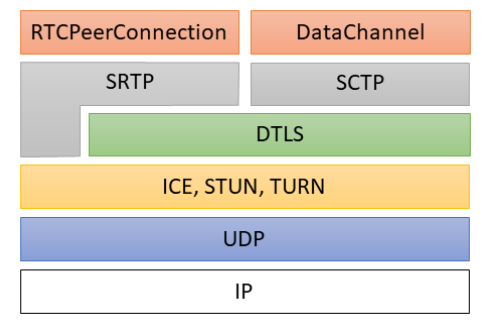
\includegraphics[width=0.4\columnwidth]{images/WebRTC connection stack.png}
	\caption{WebRTC Stack Diagram \cite{garcia2020}}
    \label{webrtc_connection_stack}
\end{figure}

\subsection{SCTP}

A core issue with WebRTC is the use of SCTP in its data channel. SCTP was originally designed for use as a signalling protocol and therefore was intended to transfer small amounts of data. This becomes problematic in scenarios where an application is required to send large amounts of data can result in critical data being blocked. \cite{webrtc_mozilla} This is relevant as although WebRTC could potentially migrate to using QUIC rather than SCTP, with new APIs designed with QUIC in mind emerging (i.e. WebTransport), it may be phased out. 

\subsection{Connection Establishment}

To establish peer-to-peer connections, WebRTC utilises the ICE algorithm which in turn makes use of the STUN and TURN protocols. Here, WebRTC attempts to make a connection directly utilising the peer address - if this fails, the ICE algorithm obtains an external address via a STUN server provided by the peer and if this fails, the algorithm finally routes traffic via a TURN relay server provided by the peer. \cite{jadhav2021} According to the documentation of Google's open-source library named "libjingle", 8\% of WebRTC connections require the use of TURN servers and therefore the end-to-end delay of a WebRTC connection is often increased due to media relay. \cite{garcia2019} This is relevant to us as QUIC achieves 0-RTT (round trip time) connection establishment - this implies that WebTransport (which uses QUIC) would have faster connection establishment than WebRTC. We know this because the ICE algorithm that WebRTC utilises is not designed with timeliness in mind. ICE will probe all of a host's candidate IP addresses and ports; although these are assigned priorities based on how likely the host thinks it is to reach a destination address, it can and often does still take a considerable amount of time. QUIC, however, is designed with timeliness as one of its main philosophies - it does not need to waste time probing as it knows exactly what it is connecting to.

\subsection{Handling packet loss with forward error correction}

In the event of packet loss, re-transmission of packets often takes too long in real-time networked applications to be useful - this is particularly prevalent in video conferencing applications where frames of video need to be played out as soon as possible. Instead, SRTP (the transport protocol utilised by WebRTC) utilises forward error correction (FEC) to combat packet loss. This works by sending additional FEC packets that contain error correcting codes alongside the original data. Then, if original packets are lost and FEC packets still arrive, the original data can be reconstructed in a timely manner. 

\subsection{Developer Experience}

Another core issue with WebRTC is that although its high-level API makes development very simple, it means that the algorithm details are hidden from developers and therefore the flexibility of WebRTC is very limited. This becomes an issue in scenarios such as the one presented in a 2013 study on WebRTC and mobile video-conferencing - this study found that WebRTC had "a heavy reliance on packet loss (among other factors) as an indicator of congestion" and that this lead to "underutilization of the wireless channel and poor video quality" \cite{fund2013}. This issue would be negated if developers had access to WebRTC's congestion control algorithm. This is relevant as WebTransport was designed to grant the developer much more flexibility by "[abstracting] away the specific underlying protocol with a flexibile (sic) set of possible capabilities" \cite{wtexplainer}.

However, other aspects of development are made significantly easier due to the widespread support of the API. Notably, further APIs have been developed to simplify various aspects of the WebRTC API - for example, PeerJS is a library that provides a configurable API built on top of WebRTC that greatly simplifies the connection establishment process from a developer's perspective. This kind of community support is not available for WebTransport as it is a far younger API - however, this may change in the future.

A key conclusion noted in several studies is that WebRTC performance degrades considerably in unstable network conditions \cite{moulay2018} \cite{jansen2018} \cite{fund2013}. This is relevant as, once again, having the capability to tailor our video conferencing applications to situations where network conditions may be unstable could be one of WebTransport's strengths.

All web-based conferencing tools today use WebRTC in some capacity \cite{gross_2020}. Popular applications such as Discord, Zoom's web client, Cisco WebEx and Microsoft Teams all utilise WebRTC in various capacities \cite{discord} \cite{webrtc_mozilla_blog}.

\section{QUIC}

QUIC is an emerging transport protocol that aims to replace TCP, TLS and parts of HTTP by acting as a secure, flexible and fast way of transporting data. QUIC supports reliable and ordered data transfer through the use of streams, and also supports unreliable, disordered data transfer by utilising datagrams. QUIC runs over UDP, but incorporates TCP's best practices, notably congestion control and time-based loss detection \cite{iyengar} (both useful features for video conferencing applications). First announced in 2012, QUIC has since been standardised in 2021.

\subsection{Streams and Datagrams}

QUIC has two main methods for transmitting data: by utilising streams \cite{rfc9000} or datagrams \cite{quic-datagrams-draft}. 

Streams provide reliable and ordered transmission of data; this is currently the main non-experimental way to transmit data within QUIC. QUIC is capable of maintaining and utilising multiple streams within a single connection - this is known as "stream multiplexing" and is a significant advantage of QUIC over TCP as it can result in more efficient data transfer. QUIC packets are sent within UDP datagrams along these streams. It is important to note that order is not preserved between these streams; for example, if a message was sent on "Stream A" before a message was sent on "Stream B", there is no guarantee that the message on "Stream A" will arrive before "Stream B"'s. However, QUIC does have the capability to prioritise particular streams and explicitly specify how queued data is transferred across multiple streams. Another important factor of QUIC streams to consider is that message boundaries are not preserved between packets. This can be disadvantageous for developers as it means that additional parsing of packets is required if developers, for example, rely on specific headers to implement application functionality. 
Streams are not ideal for real-time video transfer for numerous reasons. Particularly, their reliable nature results in re-transmission of media data when it already "has passed its play-out deadline and is no longer needed" \cite{perkins2018}. 

Datagrams provide unreliable, disordered and timely transmission of data. Currently, QUIC's implementation of datagrams is considered experimental. The draft proposing this extension states that datagrams would be useful in applications that transmit real-time data as it would combine the unreliable data transfer of UDP and the secure nature of QUIC streams. \cite{quic-datagrams-draft} 
Palmer \textit{et al.} suggest that QUIC be extended to support unreliable streams - their study proposes that there is a "clear use case for a selectively or partially reliable transport, where an application can seamlessly multiplex reliable and unreliable streams over a single connection". \cite{palmer2018} It is important to note that unreliable streams are technically different to datagrams, but the aims and overall achievements of both are the same. In a video streaming scenario, the study suggests that important frames of media data could be sent along reliable streams where as unimportant frames could be sent along unreliable streams. Palmer \textit{et al.} submitted these suggestions as a draft to the QUIC Working Group. \cite{palmerdraft}
Perkins and Ott \cite{perkins2018} advise that this proposal was flawed as it would need "relatively sophisticated APIs to offer fine-grained control of the (re-)transmission and scheduling". This is relevant as WebTransport satisfies this requirement.

\subsection{UDP Deployment}

QUIC runs over UDP for two reasons: to reduce risk of ossification due to middleboxes \cite{ossification} and to ease end-system deployment in user-space apps \cite{quic-udp-deployment}. Ossification is where developers of protocols such as QUIC reach a point where they cannot alter the protocols significantly because doing so would interact poorly with middleboxes that have come to rely on the preexisting nature of such protocols. Middleboxes are deployed by network operators to monitor and modify traffic - common examples include NATs and firewalls. Ossification is less likely to occur because QUIC is designed to make it difficult or impossible for middleboxes to interfere with QUIC connections - it does this by encrypting as much data as possible and ensuring that middleboxes therefore cannot rely on any of a QUIC packet's fields, hence preventing ossification. Additionally, UDP packets are more likely to get through firewalls than TCP packets, thus further preventing ossification. This is relevant as if we are looking for a new technology such as WebTransport to succeed WebRTC, we need to ensure that it will have significant longevity and avoid ossification. Moreover, QUIC being built on UDP further strengthens WebTransport's case for being this successor as having an easy deployment into existing or new applications is key for the potential widespread adoption of WebTransport.  

\begin{figure}[h]
    \centering
    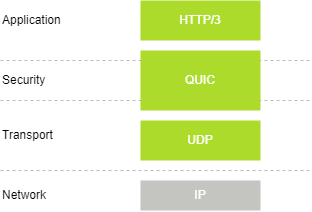
\includegraphics[width=0.5\columnwidth]{images/quic.png}
	\caption{QUIC Stack Diagram}
    \label{webrtc_connection_stack}
\end{figure}


\subsection{Connection Establishment}

A key feature of QUIC is its fast connection establishment. QUIC has a speed improvement over TLS as it combines the connection establishment and TLS handshake into 1 RTT \cite{rfc9000}. QUIC also supports 0-RTT session reestablishment \cite{quic-0rtt}. 
% \todo{Make sure this is true - work on details} 
This is relevant as one of the main conclusions of the aforementioned 2013 study on WebRTC and mobile video-conferencing was that the researchers desired a method to adapt the video data delivery depending on wireless channel conditions using all available information \cite{fund2013}.  A WebTransport implementation could utilise QUIC's 0-RTT connection reestablishment to adapt video data transmission by, for example, switching to sending data via datagrams instead of streams during periods of network instability and quickly reestablishing the session if required. This argument is further strengthened by a 2018 study that found that QUIC was able to start media streams quicker than TCP (WebRTC is likely to use TCP during connection establishment), particularly when there is congestion in the network \cite{arisu2018}. 

\section{WebTransport}

WebTransport is an API that supports streams, datagrams and communication with a remote server via a secure, multiplexed transport. WebTransport runs on top of HTTP/3, which in turn utilises QUIC extensively for data transport and connection establishment \cite{vvv-webtransport-http3-03}. WebTransport was added to Chrome 97 (stable build) in January 2022 \cite{chrome97}. The API is interacted with via JavaScript.

\subsection{Goals}

WebTransport has three goals \cite{wtexplainer}. Firstly, the API aims to provide a low latency method of communication with servers. Secondly, the API aims to be flexible; WebTransport is designed to be utilised for many use cases and with many different network protocols and data transmission configurations. This particular point is what sets it apart from WebRTC, which is less adaptable. Finally, WebTransport aims to achieve the same security properties as its contemporaries, citing WebSockets as a goal - WebSockets uses TLS and server-controlled origin policy. 
% \todo{elaborate on websockets stuff}

\subsection{Use Cases}

As mentioned before, WebTransport aims to be flexible enough to have many use cases. However, one mentioned use case from the Explainer document \cite{wtexplainer} is particularly interesting in a video conferencing scenario - this is "Receiving media pushed from server with minimal latency (out-of-order)". 

\subsection{Streams}
WebTransport is capable of utilising unidirectional and bidirectional streams via HTTP/3 in order to facilitate ordered and reliable data transfer. These streams can be initiated by either endpoint in a client/server connection. The transport of data is then facilitated via QUIC streams. \cite{vvv-webtransport-http3-03}.

\subsection{Datagrams}
WebTransport is capable of sending datagrams by utilising HTTP/3 Datagrams in order to facilitate disordered, unreliable and timely data transfer. \cite{vvv-webtransport-http3-03}. HTTP/3 sends these datagrams by employing the previously discussed experimental QUIC Datagram extension \cite{quic-datagrams-draft}. 
One potential drawback of datagrams stated by the Explainer document is that they are more suited for "small, out-of-order, unreliable messages" with "less API complexity and less network overhead than streams" \cite{wtexplainer}. Video data is quite large and may generate considerable network overhead, so it is therefore worth evaluating transmitting this data via datagrams and streams.



% can we talk about QuicTransport here?
% still not entirely sure on the relationship between the two
% say it has been added to Chrome in January
% other potential uses e.g. games

% \section{HTTP/3} 
% % do I need this?

% \section{Transferring Video Data}


% What did other people do, and how is it relevant to what you want to do?
% \section{Guidance}
% \begin{itemize}    
%     \item
%       Don't give a laundry list of references.
%     \item
%       Tie everything you say to your problem.
%     \item
%       Present an argument.
%     \item Think critically; weigh up the contribution of the background and put it in context.    
%     \item
%       \textbf{Don't write a tutorial}; provide background and cite
%       references for further information.
% \end{itemize}

%==================================================================================================================================

\chapter{Analysis/Requirements}
In this chapter, we shall outline the aims of the project and discuss how we arrived at our solution for achieving these aims. 

\section{Aims}

The main goal of this project is to quantitatively evaluate the performance of several WebTransport builds of a simple video conferencing application that use different methods for transferring data (streams, datagrams). Additionally, the project aims to evaluate a WebRTC build for comparison. Evaluation shall focus on video data transfer due to time constraints. Quantitative metrics for measuring performance shall include latency, bandwidth, loss and general performance under simulated network degradation. 

Furthermore, another key question this project aims to answer is whether or not the extra development overhead caused by utilising WebTransport makes a practical difference to the user experience or not - qualitative experiments shall be carried out to evaluate participants’ experience when using the different builds. We consider answering this question to be the secondary aim of this project.

Overall, the project aims to investigate the suitability of using WebTransport in a live video conferencing application and evaluate whether or not the effort required for using the developing API is practically worthwhile with respect to the end-user experience.

\section{Problem Analysis}

After establishing that we wanted to investigate QUIC's potential use for real-time video conferencing applications, we started researching existing technologies behind video conferencing applications and identifying their strengths and weaknesses. It quickly became clear that WebRTC is the most dominant API, with large companies such as Microsoft and Discord using it for their flagship video conferencing applications. 

However, WebRTC does not utilise QUIC, and instead utilises aging technologies such as SRTP and SCTP. Palmer \textit{et al.}'s draft \cite{palmerdraft} to the QUIC Working Group combined with Perkins and Ott's 2018 paper \cite{perkins2018} suggested to us that QUIC could be utilised effectively in video conferencing scenarios if there was an existing API to facilitate the protocol's experimental datagrams extension. After some research, we found WebTransport. We established that there was no existing formal evaluation for video conferencing applications utilising WebTransport; furthermore, there did not appear to be any formal evaluation for WebTransport at all. Reading through the documentation and working drafts of the API, we had successfully narrowed it down as being our candidate API for facilitating the use of QUIC in a video conferencing application.

\section{Requirements}

In order to achieve the project's aim of evaluating WebTransport's suitability for use in video conferencing applications, several builds of a simple video conferencing application must be developed. The "must have" and "should have" requirements of these builds are outlined as follows.

\textbf{"Must have" requirements:}
\begin{itemize}
  \item We must have a WebTransport build that sends and receives video data via datagrams.
  \item We must have a WebTransport build that sends and receives video data via streams.
\end{itemize}

These are "must have" requirements as the focus of this investigation is on how we transfer video data in WebTransport builds.

\textbf{"Should have" requirements:}
\begin{itemize}
  \item All builds should send and receive audio data.
  \item All builds should send and receive text data.
    \item We should have a WebRTC build that sends and receives video data.
    \item Builds should have functionality to host multiple clients.
\end{itemize}

The first two items relating to audio and text data are "should have" requirements as audio data and text data (for text chat functionality) are important features in a video conferencing experience. However, the scope of this project shall focus on video data due to the timescale of the project - if nothing else, suggestions for future work relating to audio and text data shall be provided.
The WebRTC build is only a "should have" requirement as it will be useful for comparison during evaluation of the WebTransport builds. However, it is not completely necessary as the WebTransport builds can be evaluated independently (although this would perhaps weaken any conclusions drawn).  
The point regarding multiple clients is a "should have" requirement mainly due to time constraints - evaluation involving a simple connection involving only two clients is adequate for evaluating WebTransport. Furthermore, it is preferable that a user survey participant only focuses on one incoming video feed so that their attention is solely on the quality of that instance, thus providing better feedback on the performances of the various underlying technologies and data transfer methods. 

\hfill

With this, we have a plan for how to achieve our aims. Developing these builds and conducting experiments on them shall fill this gap in existing research by evaluating WebTransport, specifically in a video conferencing context. Furthermore, Palmer \textit{et al.}'s \cite{palmer2018} and Perkin and Ott's \cite{perkins2018} research shall be continued - if WebTransport proves to have potential, this would provide a solution to Perkin and Ott's criticism of Palmer \textit{et al.}'s draft.  

% \section{Guidance}
% Make it clear how you derived the constrained form of your problem via a clear and logical process. 

% The analysis chapter explains the process by which you arrive at a concrete design. In software 
% engineering projects, this will include a statement of the requirement capture process and the
% derived requirements.

% In research projects, it will involve developing a design drawing on
% the work established in the background, and stating how the space of possible projects was
% sensibly narrowed down to what you have done.

%==================================================================================================================================

\chapter{Design}

In this chapter, we shall outline the various proposed builds of the application to be developed, showcase a wireframe for the user interface design and state the functional process of each build.

\section{Builds}

We shall now outline the essential and "nice to have" builds that shall be developed. 

\textbf{Essential builds:}
\begin{description}
\item[WebTransport (datagrams)]
\hfill \\
In this build, the only requirement is that video data should be sent via datagrams. 

The advantage of this is that video data shall be timely - this is important as timeliness is key to a user's experience in a video conferencing application.

The disadvantage of this build is that complex methods will need to be developed to counteract the unreliable and disordered nature of datagrams. It is indeed advantageous that WebTransport allows us to develop this ourselves, but there is no built-in solution like with WebRTC.
\hfill\\
\item[WebTransport (streams)]
\hfill \\
In this build, the only requirement is that video data should be sent via streams. 

The advantage here is that there is no need to develop complex methods for re-ordering and accounting for missing packets, as all transfer is reliable and ordered. Furthermore, streams are theoretically more capable of handling large amounts of data at once; this is particularly useful for video conferencing applications.

There is, however, a significant disadvantage here - video data will not be delivered in a timely fashion. This will likely significantly degrade the user experience as synchronisation between users occurs and the delay is too large to have any practical use in a video conferencing context.
\end{description}
\hfill\\
These builds are essential as they are necessary to achieve our project aim of evaluating WebTransport in a video conferencing scenario; we must run experiments on these builds at the very least.
\hfill\\

\textbf{"Nice to have" builds:}
\begin{description}
\item[WebRTC]
\hfill \\
There are several requirements for this build. Firstly, it shall include video, audio and chat (text) data. Video and audio data should be sent via the API's media channel, and chat data should be sent via the API's data channel. Next, the connection should be peer-to-peer. Finally, any external libraries and packages that may simplify development should be used.

The advantage of this build is that it should be considerably easier to develop than the WebTransport builds. Particularly, the use of external libraries and packages should further assist the developer.
\hfill\\
\item[WebTransport (streams and datagrams) Build 1]
\hfill \\
In this build, we shall transmit video and audio data. The general aim of this build (and the following two) is to explore how different data can be transmitted via different mediums, and examine the advantages and disadvantages of each configuration.

Video data should be sent via streams and audio data should be sent via datagrams. Chat data is irrelevant for this build - the focus here is on evaluating video vs audio data. 

The advantage of sending audio data via datagrams is that audio (more specifically speech) data is highly loss tolerant - it can conceal 10-20\% random packet loss without noticeable loss in quality, and speech is still legible with 50\% loss. Video data loss is harder to conceal, although users tend to be more lenient with video issues than audio issues \cite{730750}. The specific aim of this build is to evaluate how video and data being sent in this configuration contributes to the user experience. 

A disadvantage of this build is that, again, video data sent on streams is untimely and results in a degraded user experience. It will be interesting to examine the trade-off between timeliness and reliability with respect to video data and see what users prefer. Additionally, it will be interesting to see if users do not mind large loss of speech data. 
\hfill\\
\item[WebTransport (streams and datagrams) Build 2]
\hfill \\
In this build, video data should be sent via datagrams and audio data should be sent via streams. Chat data is once again irrelevant in this build for the same reason as before. The specific objective of this build is to evaluate the differences with the previous build and help answer the same question.
\hfill\\
\item[WebTransport (streams and datagrams) Build 3]
\hfill \\
In this build, video and audio data should be sent via streams and chat data should be sent via datagrams.

The specific objective here is to evaluate WebTransport's statement in the Explainer document \cite{wtexplainer} that datagrams are more suited for small messages whereas streams are better suited for large. The results here would help us evaluate whether sending video data via WebTransport's datagrams implementation is viable or if it is better suited for small items such as text data.
\end{description}
\hfill\\
% \todo{WebRTC system diagram?}
These builds would strengthen the project's results, but are not necessary to achieving our aim of evaluating WebTransport. The WebTransport builds here would help further evaluate the API, but may be out of scope for this project due to time constraints; it is more important to get the minimum evaluations required to achieve a comprehensive evaluation (i.e. from the essential builds).

\section{User Interface}

Figure \ref{wireframe} illustrates a wireframe for the appearance of each build. As this project is more research-oriented, the final application will not have a focus on user experience or user interface design. Consequently, we will not consider any metrics related to usability or aesthetic. Instead, the focus will purely be on the quality of video, audio and text data sent and received.

\section{WebTransport - How the builds work}
Figure \ref{wt_systemdiagram} illustrates a high-level overview of how the WebTransport builds shall work. 

\begin{figure}[h]
    \centering
    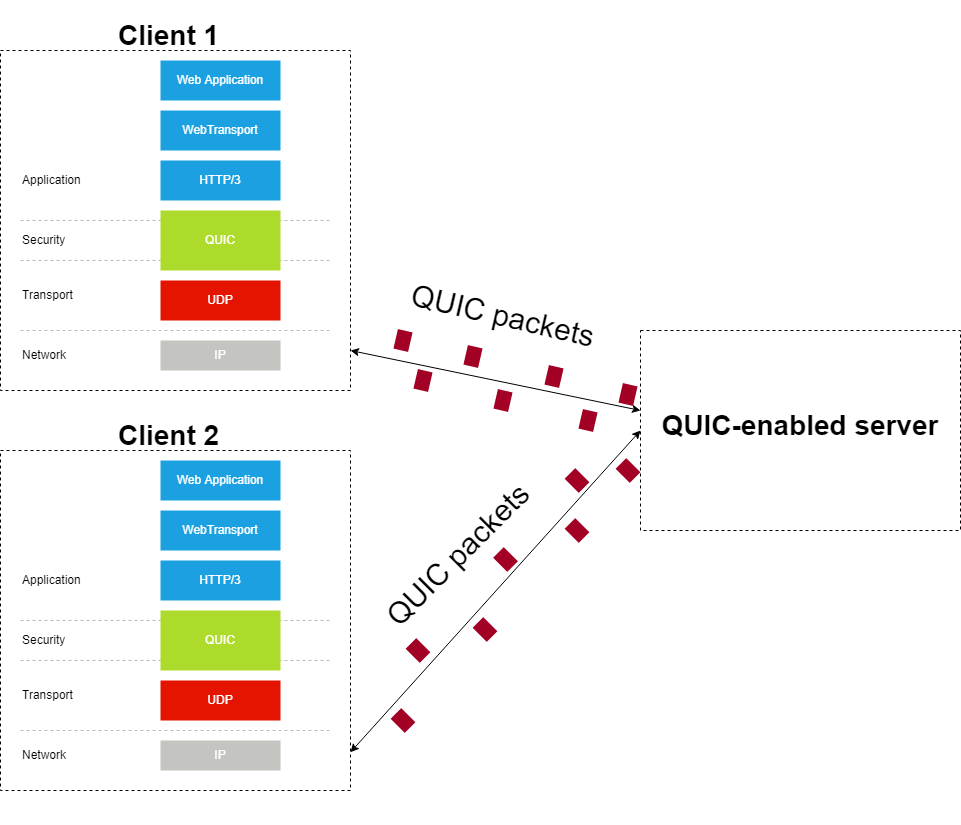
\includegraphics[width=0.7\columnwidth]{images/webtransport build diagram.png}
	\caption{System Diagram for WebTransport builds.}
    \label{wt_systemdiagram}
\end{figure}

On the left side of this diagram, we can see our two clients - each of these are a JavaScript web page running on Google Chrome browser windows. On the right side, we can see our QUIC-enabled server - this shall receive data from each client and forward this data to the other client. We shall explore several existing QUIC server implementations written in different languages whilst developing this server.

The general working pattern of our builds is simple. Clients will establish a connection to the server, transmit data and be ready to receive data - once both clients are connected, the server shall forward received data to each client in order to establish an information flow similar to the one illustrated in Figure \ref{wt_systemdiagram}. 

In Figure \ref{wt_systemdiagram}, the bidirectional arrows between each client and server represent what will either be WebTransport's streams implementation or its datagrams implementation. The diagram represents both builds and the general workflow of both is the same - the only difference is what the QUIC packets will be sent via.

We shall now outline high-level overviews of how the data will actually be sent and received by the WebTransport clients. There is a significant amount of shared functionality between the Datagrams and Streams builds, so this shall be covered first. Specifically, the two builds send data in almost the same way. After this, we shall diverge and talk about the design choices unique to each build.

\subsection{Sending Data - Datagrams and Streams Builds}

Firstly, our client requests and accesses the user's camera. Then, at regular intervals, the client shall send data generated from the user's media feed to the server. This data will be a frame of image data and some arbitrary amount of audio data. Then, the client shall encode this data into chunks and send these chunks as packets until a full frame of video data and the full amount of audio data have been transmitted. This is illustrated in Figure \ref{wt_sending data} - here, a chunk of data (at an arbitrary position for illustration purposes) is taken from our frame of image data, packaged into a packet and transmitted to the server via either WebTransport's streams or datagrams implementation.

\begin{figure}[h]
    \centering
    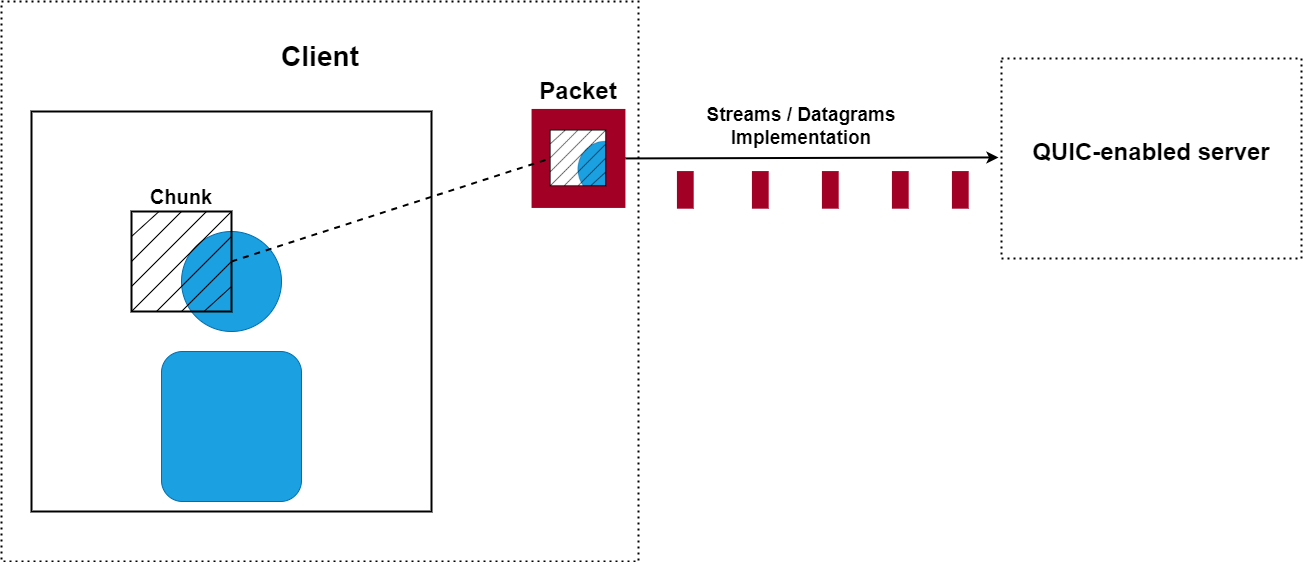
\includegraphics[width=0.9\linewidth]{images/sending data.png}
	\caption{An illustration of how WebTransport clients encode and transmit video data.}
    \label{wt_sending data}
\end{figure}

Additionally, header values shall prelude the data in these packets - specifically, these header values shall be a user ID, a packet sequence number, a frame number, a timestamp and an integer value (we shall call this eof) indicating whether the frame and chunk has been fully sent. During and after this process, relevant header data shall be updated continuously; specifically, the sequence number increases as packets send, the frame number increases as frames send and the eof sets to 1 when a frame and chunk have finished sending. Meanwhile, at the rate of the specified regular interval, more frames and audio data will be getting queued to be decomposed and sent. This process is applicable to sending data via both datagrams and streams.

Whilst this is occurring, the server shall be receiving this data and passing it on to the other connections in the session. We shall now examine how the WebTransport clients handle received data.

\subsection{Receiving Data}
The client shall constantly be waiting to read data. When data is received, the way it is handled depends on the specific build - the builds are similar, but the Datagrams build has a lot of extended functionality to handle the disordered and unreliable nature of datagrams. We shall now examine how data is received in each build, starting with the Streams build.
\hfill\\
\subsubsection{Receiving Data - Streams Build}
\hfill\\
The Streams build will handle receiving data more simply than the Datagrams build. 
The client will first check if a maintained buffer offset variable in addition to the size of the received data is greater than the size of the received frame. If it is, the received data will be cut down so that only the data that is necessary to receive a full frame is read. The leftover data will be stored in another variable. This will only happen when the last necessary packet to receive a full frame is read and prevents unnecessary data being processed. 

Then, the client shall add the received data to a buffer at a specified offset value. This offset value will then update to accommodate for the new data in the buffer. 

\begin{figure}[h]
    \centering
    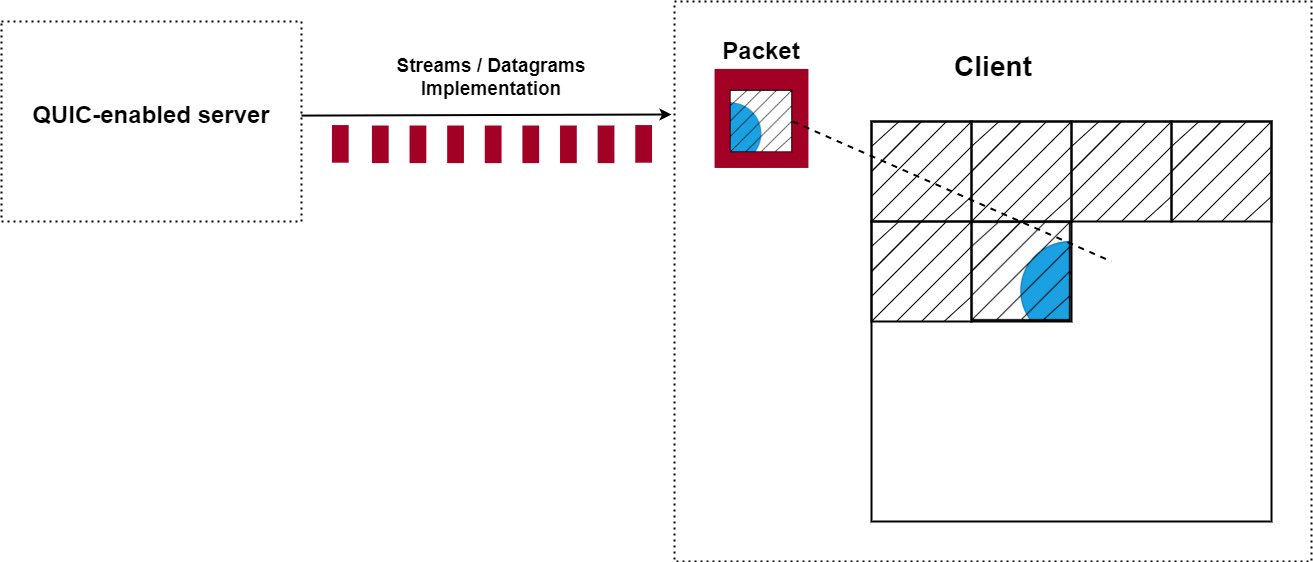
\includegraphics[width=1\linewidth]{images/receiving data.png}
	\caption{An illustration of how WebTransport clients receive video data and builds up a frame.}
    \label{wt_receive data}
\end{figure}


The client shall repeat this process until the buffer offset is equal to the size of the received frame. Then, the client will render this complete frame and the buffer offset and buffer shall return to their first states. An illustration of how a frame is built up can be seen in Figure \ref{wt_receive data}. 

Finally, the leftover data (which belongs to the next frame) is added to the buffer and the whole process repeats. This is done to ensure that no received data is wasted. We can operate this way because we know that all data will be received due to the reliable nature of streams. A similar process shall be undertaken for audio and chat data.

% \todo{is this too technical - should details of e.g. buffer offsets and leftover data belong in implementation?}

We shall now examine how the Datagrams build receives data.
\hfill\\
\subsubsection{Receiving Data - Datagrams Build}
\hfill\\
The Datagrams build operates in the same way as the Streams build, but has some additional complexity that handles packet loss and reordering.
The client shall extract the headers from the received packet - this is achievable as datagrams, unlike streams, preserve message boundaries.The client shall use these headers to gain knowledge on what frame number the packets currently being processed are from - this information shall be utilised to reorder packets and create some sort of "timeout" for frames that take too long to have data be retransmitted. To elaborate, if, for example, "Frame 8" takes too long to have the last third of its data be transmitted (thus disrupting the user experience), the client shall know to render what they have of "Frame 8" and move on to queued data from "Frame 9". An illustration of this can be seen in Figure \ref{wt_design_latepackets}.

\begin{figure}[h]
    \centering
    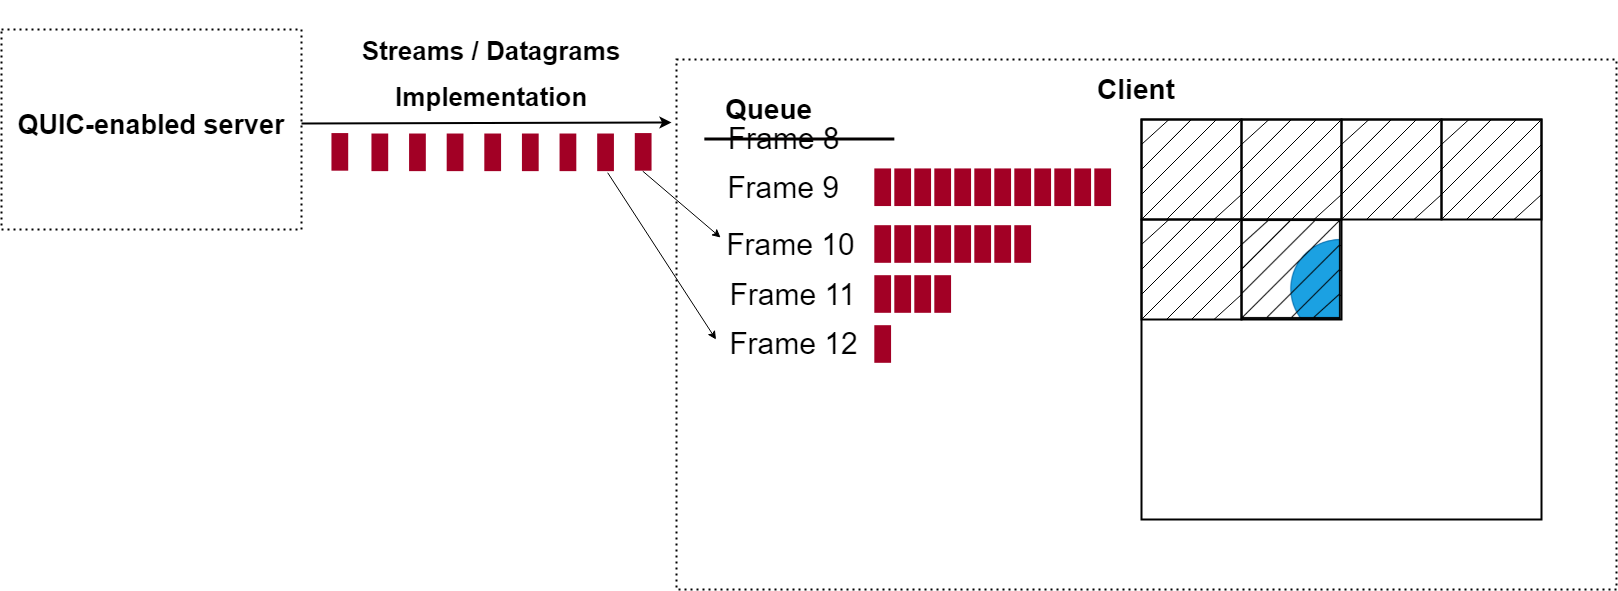
\includegraphics[width=1\linewidth]{images/late packets.png}
	\caption{An illustration of how WebTransport clients discard packets of a certain frame after an arbitrary timeout.}
    \label{wt_design_latepackets}
\end{figure}

The client shall continue building a frame even when data is lost. It does this by altering the buffer offset to account for where the lost data should have been inserted into the buffer. An illustration of this can be seen in Figure \ref{wt_design_shifteddata}.

\begin{figure}[h]
    \centering
    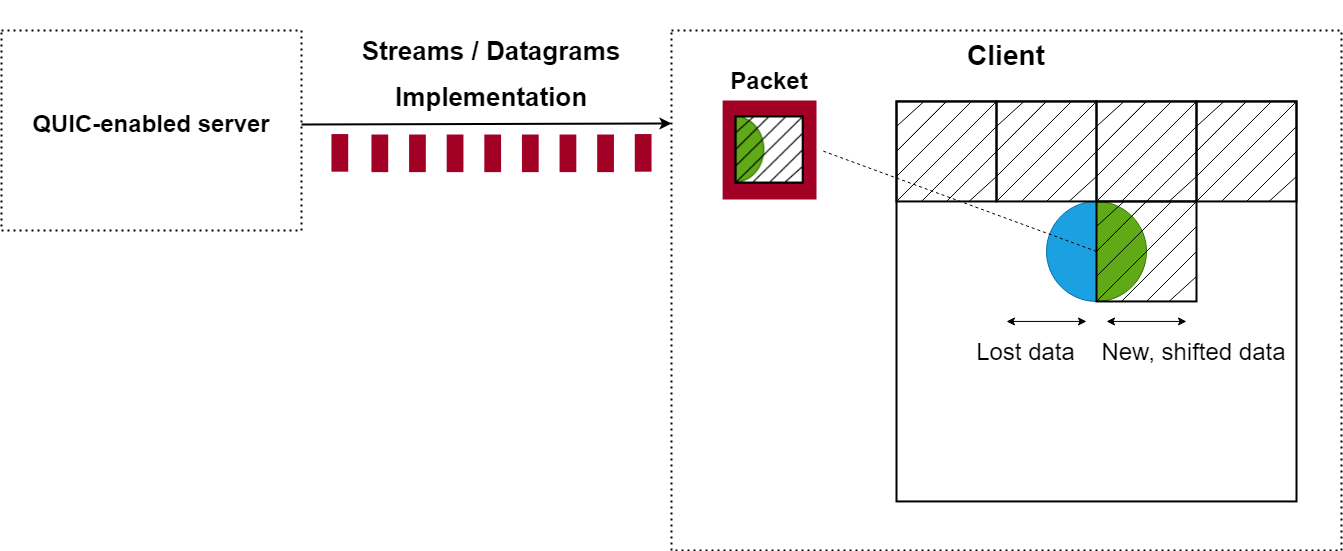
\includegraphics[width=1\linewidth]{images/shifted data.png}
	\caption{An illustration of how WebTransport clients shift received data to deal with lost packets.}
    \label{wt_design_shifteddata}
\end{figure}

This combination of techniques to handle loss and reordering should prove as adequate measures for combatting the unreliable and disordered nature of datagrams. Chat and audio data shall be handled similarly, although chat data particularly will not require such complex handling.

This summarises how the WebTransport builds shall send, receive and display data. We shall now examine how the WebRTC build shall work.

\section{WebRTC - Process}
Developing the WebRTC build shall be a much more high-level and simple experience, utilising available libraries and extensions to WebRTC as well as existing online tutorials. My reasoning for this is that a factor in the evaluation of WebTransport's potential is the developer's experience - WebTransport may facilitate more effective video transfer, but extra development overhead may make it undesirable for software developers to actually make use of it. Because of this, I shall make use of existing libraries and tutorial resources to allow for comparison between the development experiences of projects utilising WebRTC and WebTransport.

% \subsection{PeerJS}
% From a developer's perspective, PeerJS greatly simplifies WebRTC's connection establishment process - PeerJS allows developers to create a peer-to-peer media stream connection utilising nothing but this ID. This library provides a JavaScript API. In the application, we shall generate this unique ID and use it to connect to our peer.

% \subsection{socket.io}
% socket.io is a JavaScript library that enables real-time, bi-directional communication between web clients and servers. socket.io utilises WebSockets - this is an established API that allows for reliable, ordered and untimely data transfer between a client and a server in a single stream. WebSockets is similar to WebTransport, but is not as customisable, suffers from head-of-line blocking and transports data via TCP rather than QUIC \cite{websockets_mozilla_docs}, thus making it generally unsuitable for media transfer.

% In our application, we shall utilise socket.io to facilitate the communications relating to setting up "rooms" for users to join. These rooms will again be based on a unique ID generated by the application. 

The application shall set up a server that facilitates communication of logic relating to "rooms". These rooms will act as sessions for different clients to exist in - they shall be created when a client starts a new session and automatically generates a unique ID that acts as the "room ID". Our reasoning for including rooms is that it shall showcase the widely available and open source additional functionality in WebRTC projects (something not yet seen with WebTransport). Once routed to the correct room, a client shall have another unique ID generated to correspond to their "user ID". The client shall then have the user's media feed accessed and displayed. Once a second client connections, the clients shall establish a peer-to-peer connection to each other and media data shall be exchanged. Each client shall receive the others' media data and this will be displayed alongside their own media feed. Chat data shall be sent utilising WebRTC's data channel, and media data shall be sent via WebRTC's media channel.

\hfill{} \\
Thus concludes all of our designs. Due to the relative lack of existing research on the subject area, we recognise that it is hard to determine how many of these builds we will be able to implement within the timescale of the project. This is because it is unknown how much difficulty we will have with development, particularly for the WebTransport builds. However, we decided that we would rather design too many builds to evaluate than too little, and implement as many as we can in order of importance.


% How is this problem to be approached, without reference to specific implementation details? 
% \section{Guidance}
% Design should cover the abstract design in such a way that someone else might be able to do what you did, 
% but with a different language or library or tool. This might include overall system architecture diagrams,
% user interface designs (wireframes/personas/etc.), protocol specifications, algorithms, data set design choices,
% among others. Specific languages, technical choices, libraries and such like should not usually appear in the design. These are implementation details.


%==================================================================================================================================

\chapter{Implementation}

In this chapter we shall outline which builds specified in the design were implemented, and examine how they were done so with detailed reference to the methods and technologies used. 

\section{Resources Used}
To aid development, we utilised several existing solutions as bases for our implementations. In particular:
\begin{itemize}
    \item \textbf{Google's Sample WebTransport Client} \cite{wt_js_client_sample} was used as the basis for our WebTransport builds' client code. This code implements a basic event log, provides several functions for sending and receiving both datagrams and stream data and establishes the WebTransport connection. 
    \item \textbf{web-platform-test's WebTransport-compatible QUIC-enabled python server} \cite{web-platform-tests} was used as the basis for our WebTransport builds' server code. web-platform-test is a test suite that allows developers to run several automated tests on their servers to ensure they are robust and capable - we do not utilise these tests, but we do make use of the provided server. This code handles all the basic server logic.
    \item \textbf{Web Dev Simplified} \cite{web_dev_simplified} provided a video tutorial on how to set up a WebRTC video conferencing application. This was used to develop our WebRTC build and was not significantly further built upon.
\end{itemize}
\hfill{} \\
We shall now examine how our WebTransport builds were implemented.

\section{WebTransport}

Our WebTransport builds meet our previously defined "must have" requirements - we have a build that sends and receives video data via datagrams and one that does the same via streams. However, the builds do not meet any of our "should have" requirements. Firstly, due to time constraints, they do not send or receive audio or text data. Secondly, the datagrams build does actually support multiple users in one session, but is not optimised to do so. Finally, the streams build does not support multiple users in one session at all - this was because of the way packet headers are sent via streams, which we shall discuss later in the paper. 

% \begin{figure}[h]
%     \centering
%     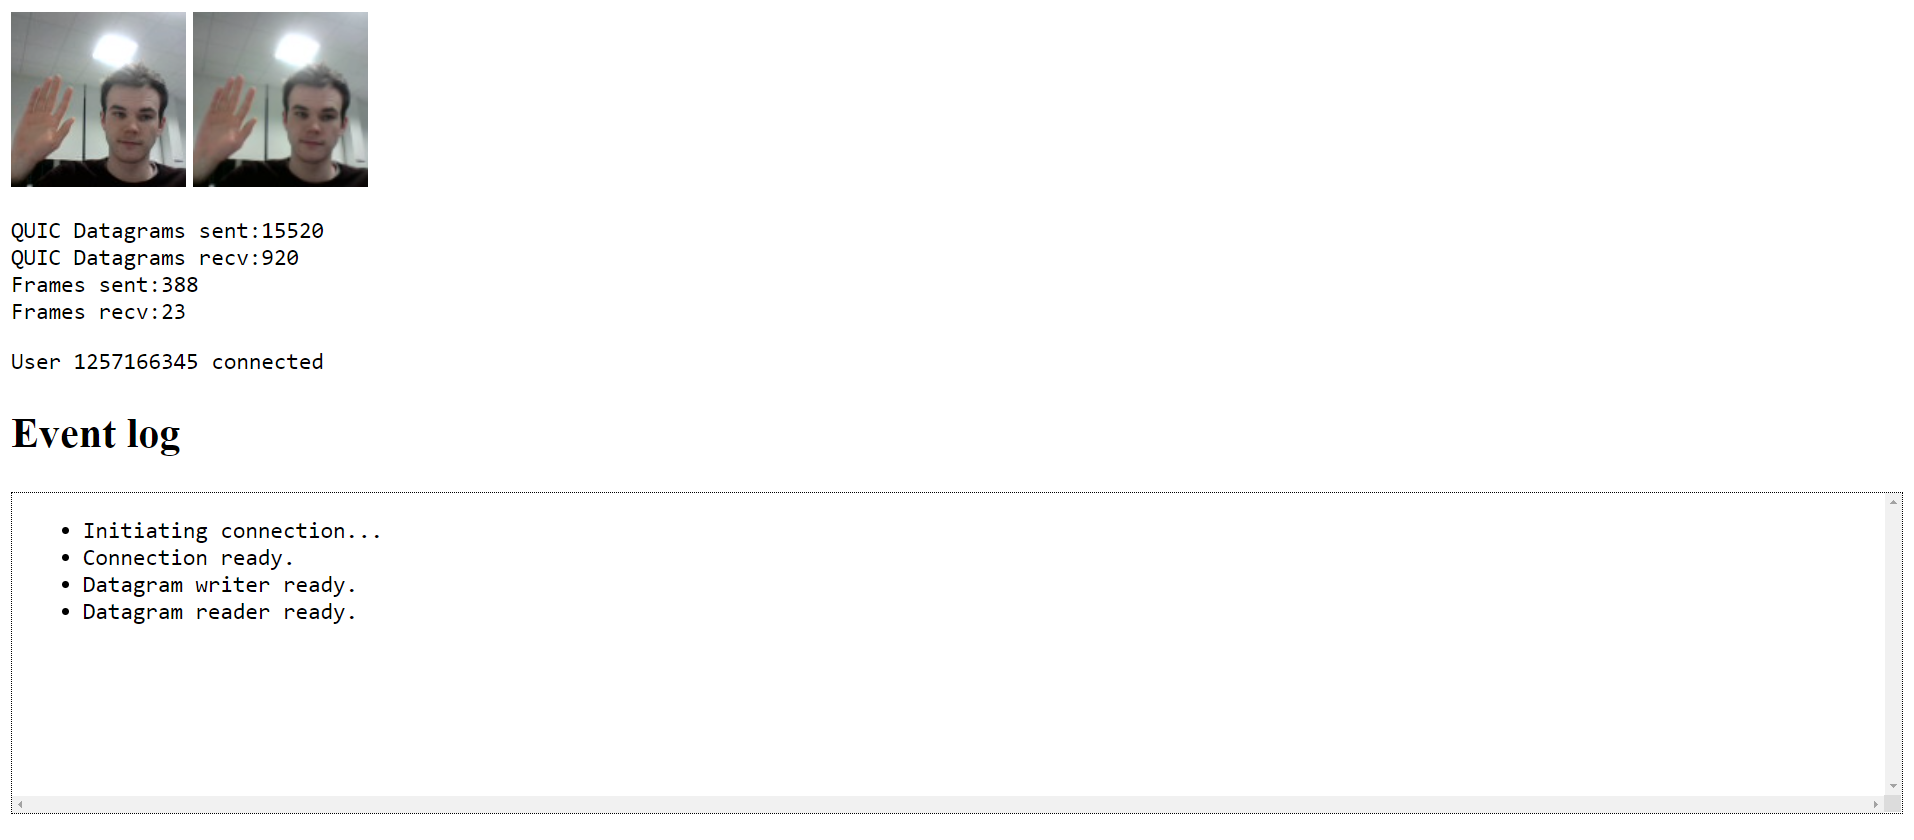
\includegraphics[width=0.95\linewidth]{images/webtransport build.png}
% 	\caption{A screenshot of the WebTransport build.}
%     \label{wt_build_screenshot}
% \end{figure}

The final design of the WebTransport builds is close to the initial wireframe (as seen in Figure \ref{wireframe}), albeit without the chat log (as this was not implemented). Additionally, the high-level system operation is consistent with the system diagram given in our Design chapter, specifically illustrated in Figure \ref{wt_systemdiagram}.

In this section, we shall first examine the shared functionality between the two builds. The server used by the two builds is actually the same, so we shall start with discussing this and how it supports both datagrams and streams. Following this, we shall examine our two WebTransport clients - one for the Datagrams build, and one for the Streams build. Again, there is some shared functionality here, so this shall be examined before diverging into build-specific functionality.

\subsection{WebTransport Server}
The base server provided by web-platform-tests is effective, yet limited. It is a WebTransport over HTTP/3 server written in python - it utilises the aioquic library \cite{aioquic} to implement QUIC and WebTransport functionality. It is capable of establishing a connection, receiving data via datagrams or streams and sending that data back to the original sender. As it is capable of handling both datagrams and streams data, we use this as the basis for both our Datagrams and Streams WebTransport builds.

Our expansion added the functionality to send received data to other existing connections. It did so by keeping a list of session objects and sending data to each session object that was not the sender's own session.

\begin{lstlisting}[language=python, caption={Added server functionality of sending data to other existing connections (streams example).}, label=lst:callahan]
    ...
    
    session = WebTransportSession(self, counter, request_headers)
    connections.append(session)
        
    ...
    
    for connection in connections:
        if connection != self._session:
            if (self._session.stream_is_unidirectional(stream_id)):
                pass
            else:
                connection.send_stream_data(stream_id, data, stream_ended)                    
                self._run_callback("stream_data_received", stream_id, data, stream_ended)

\end{lstlisting}
    
Another significant expansion was the ability for the server to read the packet headers sent to it. This was tailored for my client implementation and so worked with DataViews and 32-bit unsigned integers (this will be explained further in the paper). The function worked by putting the received data into a DataView class defined in python and then decoding the contents to extract multiple 32-bit unsigned integer at various byte offsets. These integers corresponded to the packet's headers. This code can be seen in Listing \ref{lst:server-decode-headers}. Ultimately, this feature was not utilised in any of our final builds. However, in future, it could be useful for implementing specific server logic in WebTransport applications - for example, in a scenario where connection becomes unstable, the server could receive some header indicating that it should send received data back utilising streams instead of datagrams to ensure reliability over timeliness. Furthermore, it is useful for logging and testing purposes.

\subsection{WebTransport Clients}

We shall now examine how the WebTransport clients operate and what shared functionality there is between the Datagrams and Streams builds. The two builds send data in similar fashion but receive data slightly differently, so we shall explain the sending process of both builds before diverging to talk about the two receiving processes.
\hfill\\
\subsubsection{Sending Data - Datagrams and Streams Builds}
\hfill\\
After establishing the connection to the server, the client immediately requests the video data from the user's camera and generates a unique user ID. Then, the client sends single frames of video data at a regular arbitrary interval by repeatedly calling the \textit{sendData} function - we found that 100ms worked suitably (resulting in an output of 10 frames per second) and used this for our evaluations later. This was an arbitrarily chosen value. 

\textit{sendData} works by utilising a while loop; this loop continues to send data until a variable, \textit{offset}, is found to be greater than the length of the image data. This works in two stages.

Firstly, at the start of every loop, the \textit{size} variable is used to signify the size of the sent packet. We chose \textit{size} to have a value of 1004 as our headers take up 20 bytes, and we decided to have our packets be 1024 bytes long (this was an arbitrarily selected value). Then, the following \textit{if} statement checks if \textit{offset} in addition to \textit{size} is greater than the length of the image data. If it is, \textit{size} is decreased to only send the required amount of image data to complete a full frame. A representation of this process can be seen in Figure \ref{wt_sending_trimchunk}, and the code that alters \textit{size} is seen in Listing \ref{lst:resize}.

\begin{figure}[h]
    \centering
    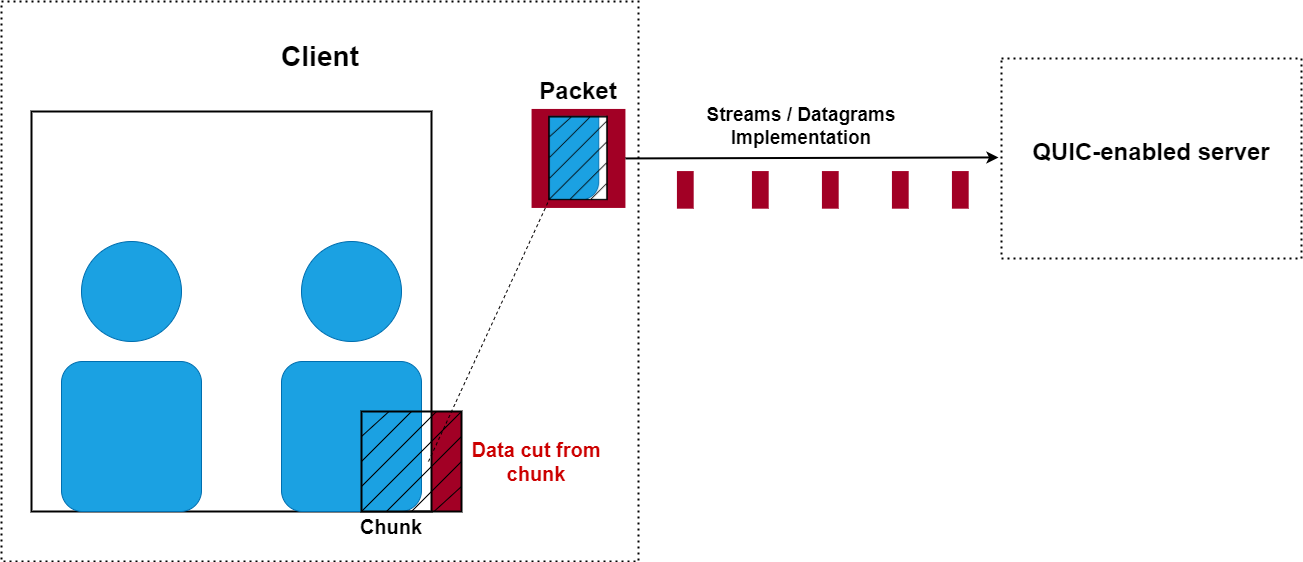
\includegraphics[width=0.95\linewidth]{images/cutting chunk sending.png}
	\caption{The WebTransport client resizing sent chunk to only send what is necessary to complete a frame.}
    \label{wt_sending_trimchunk}
\end{figure}

\hfill{} \\

\begin{lstlisting}[language=javascript, caption={First part of functionality that exits loop when full frame is sent.}, label=lst:resize]
    let size = 1004;
        if (offset + size > imgData.data.length) {
            size = imgData.data.length - offset;
    }

\end{lstlisting}

The second stage is at the end of the loop; here, after a chunk of data is sent, the client adds the \textit{size} of the sent chunk and checks if \textit{offset} is now greater than the length of the image data. If so, this indicates that the full frame is sent, the loop is exited and the client moves on to sending the next frame.  This is seen in Listing \ref{lst:second_stage}.

\begin{lstlisting}[language=javascript, caption={Second part of functionality that exits loop when full frame is sent.}, label=lst:second_stage]
    offset += size;
    if (offset >= imgData.data.length) { 
        break;
    }
\end{lstlisting}

Now, we shall examine how each chunk is encoded and sent. A chunk is encoded by slicing the image data between the current \textit{offset} and the succeeding amount of data according to \textit{size}. An illustration of this can be seen in Figure \ref{wt_sending_chunkoffset}.

\begin{figure}[h]
    \centering
    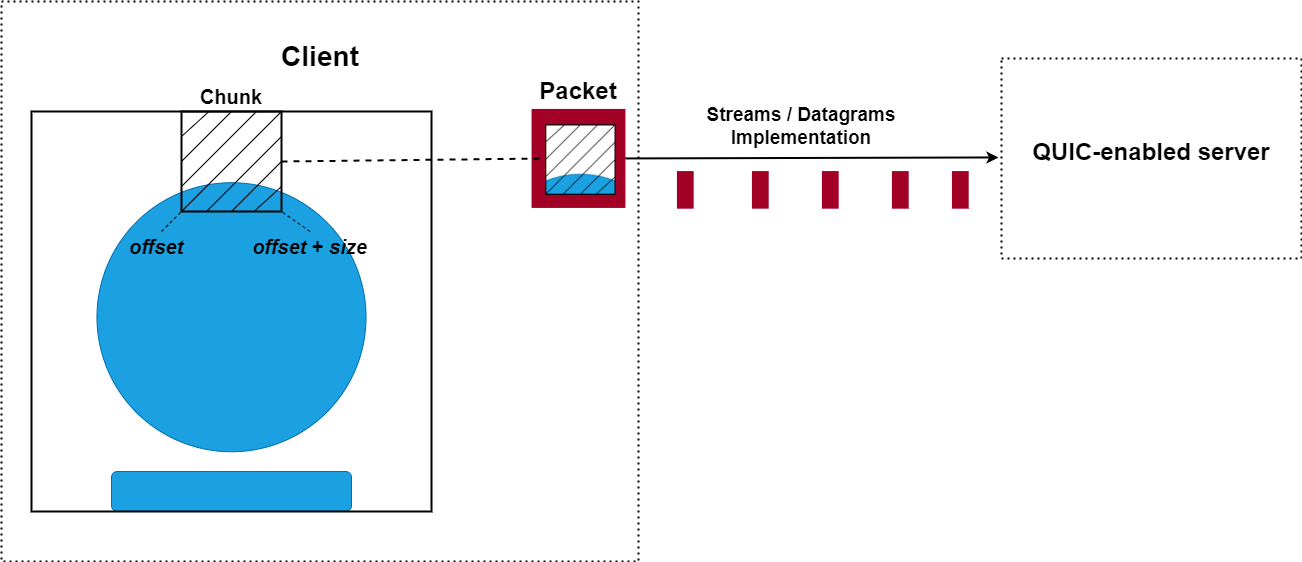
\includegraphics[width=0.95\linewidth]{images/how chunk is selected.png}
	\caption{The WebTransport client selecting a chunk of data to process.}
    \label{wt_sending_chunkoffset}
\end{figure}

Then, a buffer \textit{writeBuffer} is created. This buffer is an \textit{ArrayBuffer} and is stored within a \textit{Uint8ClampedArray} - this array is the length of a predefined header size (\textit{HEADERSIZE}) in addition to the value of \textit{size}. We use a \textit{Uint8ClampedArray} simply because our received image data is stored in a \textit{ImageData} object, whcih also utilises a \textit{Uint8ClampedArray}.

Then, this buffer is put into a \textit{DataView}. We use the \textit{DataView} here as an API of sorts to access the bytes at different arbitrary byte-positions; this is useful as we insert and extract headers for later processing. For the Datagrams build, we insert our headers into the first 20 bytes of the packet. Our headers are \textit{streamId} (the predefined unique user ID), \textit{sequenceNumber} (the sequence number of the packet within the frame), \textit{eof} (a boolean indication of whether the frame has been fully sent), \textit{frameNumber} and \textit{ts} (a timestamp of when the packet was sent from WebTransport). The packet is then sent, thus concluding our data transmission algorithm. 

\begin{lstlisting}[language=javascript, caption={The encoding and transmission of our video data.}, label=lst:callahan]
    const chunk = imgData.data.slice(offset, offset + size);

    let writeBuffer = new Uint8ClampedArray(HEADERSIZE + chunk.length);
    const dv = new DataView(writeBuffer.buffer, 0);

    writeBuffer.set(chunk, HEADERSIZE);
    
    sequenceNumber++;

    dv.setUint32(0, streamId);
    dv.setUint32(4, sequenceNumber);  
    dv.setUint32(8, offset + size >= imgData.data.length ? 1 : 0); // eof
    dv.setUint32(12, frameNumber);
    dv.setUint32(16, (Date.now()/1000));

    await currentTransportDatagramWriter.write(dv); 
\end{lstlisting}

It is important to note here that we do not utilise headers in our Streams build as message boundaries are not preserved and headers are consequently useless for later processing. Although a way around this may be explored in future, there is no reasonable way to extract these headers within the scope of this project.

We shall now examine how each build receives data. The two builds are essentially the same, but the Datagrams build has added functionality to handle packet reordering and loss. Because of this, we shall examine the shared functionality between the two before discussing the Datagrams build's unique features.
\hfill\\
\subsubsection{Receiving Data - Datagrams and Streams Builds}
\hfill\\
The client receives data as often as it can, reading data as soon as it is available in a while loop that only exits when the connection is closed. 

If a new \textit{streamId} is detected, the client generates a new video feed and renders all incoming data in this feed. One distinction here is that the Datagrams build reads the unique \textit{streamId} from the packet headers, whereas the Streams build just defines this itself as either "1" or "2" - this is why the Streams build is incapable of handling more than two users in one session. 

A dictionary, \textit{connections}, is used to track each user session - each dictionary contains an associated \textit{buffer} and \textit{bufferOffset}. 

These are all the similarities between the two builds. We shall now discuss the builds separately.
\hfill\\
\subsubsection{Receiving Data - Streams Build:}
\hfill\\
We shall refer to the data inside a received packet as \textit{value} from here on. Similarly to before with \textit{offset} and \textit{size} (see Figure \ref{wt_sending_chunkoffset}), we check to see if the connection's \textit{bufferOffset} in addition to the \textit{dataSize} (the size of \textit{value}) is greater than the size of the frame (\textit{FRAMESIZE)} - if it is, we amend the size of the data array we are reading and use this to update our \textit{buffer} later. This is done to ensure that we do not add more data to the generated frame than necessary. Next, the connection's \textit{buffer} has \textit{value} appended to it (sliced according to the potentially altered \textit{dataSize}) at an index of \textit{bufferOffset}. Then, \textit{bufferOffset} is increased by the value of \textit{dataSize}. The remaining data that is cut off when we sliced \textit{value} is then added to another array, \textit{leftoverData}, which we will use later. The code for this process can be seen in Listing \ref{buildingbuffer}. The purpose of all this is to "build up" the \textit{buffer} until we have all the data needed to render a full frame.

\begin{figure}[h]
    \centering
    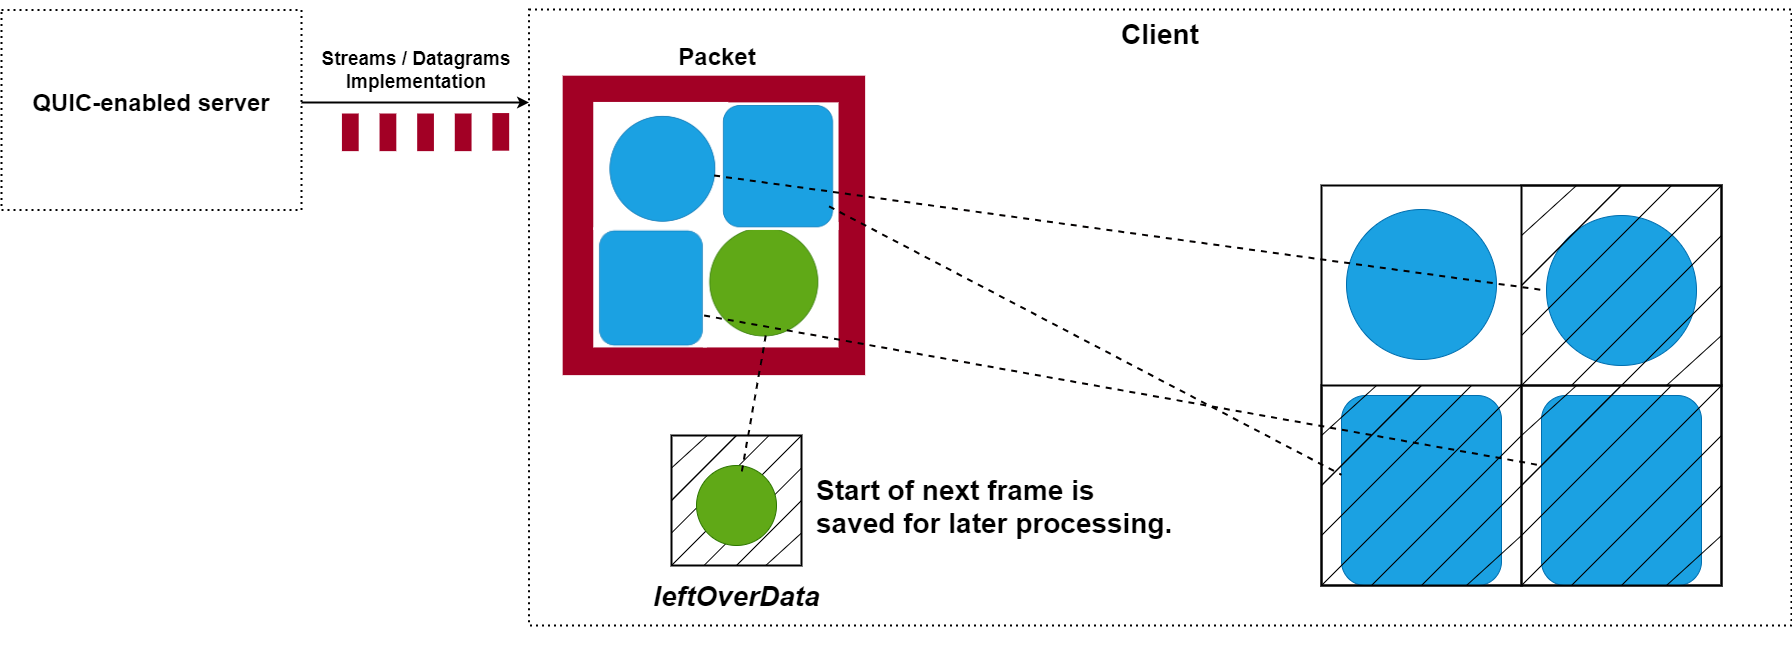
\includegraphics[width=1\linewidth]{images/wt_streams_leftoverdata.png}
	\caption{The WebTransport client building up a frame whilst working without message boundaries (streams).}
    \label{wt_streams_leftoverdata}
\end{figure}

\begin{lstlisting}[language=javascript, caption={Streams build's client building up the buffer.}, label=buildingbuffer]
    if (connections[streamId].bufferOffset + dataSize > FRAMESIZE) {
      dataSize = FRAMESIZE - connections[streamId].bufferOffset; 
    }
    connections[streamId].buffer.set(value.slice(0, dataSize), connections[streamId].bufferOffset);
    connections[streamId].bufferOffset += dataSize;

    leftoverData = value.slice(dataSize, );
\end{lstlisting}

\textit{leftoverData} is necessary as, once again, streams do not preserve message boundaries. Consequently, chunks sent from the other client are encapsulated arbitrarily into packets, meaning that a chunk does not arrive in the exact packet it is sent in; this is illustrated in Figure \ref{wt_streams_leftoverdata}. This results in some packets containing data from parts of multiple chunks, meaning we must employ additional parsing of received packets. 

Next, we will check if \textit{bufferOffset} is equal to \textit{FRAMESIZE}; if it is, we have all the data necessary to comprise a full frame and so the frame is rendered. Once the frame is rendered, \textit{bufferOffset} is reset.

Finally, if this occurs and there is some data in \textit{leftoverData}, we essentially redo the process of Listing  \ref{buildingbuffer} - this ensures that no data is wasted and the next frame does not have any data missing from the start of its \textit{buffer}. Then, \textit{leftoverData} is reset and the process begins again.

The client for the Streams build was far easier to implement than the Datagrams build counterpart.
\hfill\\
\subsubsection{Receiving Data - Datagrams Build}
\hfill\\
The Datagrams build's client has the same general process of adjusting \textit{bufferOffset} and \textit{buffer} depending on \textit{dataSize} and rendering when the end of the frame is reached. Regarding the latter point, this is done via the \textit{eof} header; furthermore, the rest of the headers are used throughout the client (unlike with the Streams build). In particular, the Datagrams build is capable of hosting multiple connections as it is able to render new video feeds based on the unique \textit{streamId} header by creating a new video feed and \textit{connection} dictionary whenever a new unique \textit{streamId} is detected.

We shall now examine the main feature of the Datagrams build that sets it apart: the techniques that handle packet loss and disorder. 

The client handles packets arriving in a disordered fashion by creating a queue - this queue is a dictionary of arrays with each key corresponding to a frame number and each value storing an array containing the relevant packets. This dictionary shall be referred to as \textit{dict}. A new key/value pair is created every time a new \textit{frameNumber} is detected. As new datagrams come in, if the \textit{value} (i.e. the payload data from a datagram) is not present in the dictionary (i.e it is not a duplicate datagram) and the \textit{frameNumber} has not been discarded (more on this later), the \textit{value} is added to the queue. The queue is constantly maintained in an ascending order by sorting the keys every time a new \textit{value} is added. Next, to actually process the datagrams in order, the client attempts to take the first \textit{value} from the lowest present \textit{frameNumber}. If it succeeds, the datagram shall be handled as normal until \textit{eof} is received - once the frame has been completed, the \textit{frameNumber} is deleted as a key value from \textit{dict}, the frame is rendered and the process restarts. This process is very similar to the one outlined in Figure \ref{wt_design_latepackets}.

However, what if the frame is not completed and there are no datagram \textit{value}s in the queue for the lowest \textit{frameNumber}? This may occur when packets, notably one containing the \textit{eof} header, are lost. To combat this, the client implements an arbitrary timeout on each \textit{frameNumber} - this is set to 10 retries. If the client attempts to read these missing datagrams 10 times and none arrive, the \textit{frameNumber} is discarded from the queue and added to an array of discarded frames, \textit{forgottenFrames} - this array is used in the earlier \textit{if} statement to discard datagrams that correspond to these "timed out" frames. The code for this process can be seen in Listing \ref{lst:discarding_frames}.

\begin{lstlisting}[language=javascript, caption={Datagrams build's client handling timed out frames.}, label=lst:discarding_frames]
    value = dict[keys[0]].shift();
    if (!value) {
      counter++;
      if (counter == 10) {
        forgottenFrames.push(prevFrameNumber)
        render(connections[streamId], frameNumber);
        delete dict[keys[0]];
        counter = 0;
        prevSequenceNumber = 1;
      }
      continue;
    }
\end{lstlisting}

The client also handles packets that go missing during the construction of a frame (i.e. in the scenario where the start and end of the frame still arrive). It does this by keeping track of a variable, \textit{prevSequenceNumber} in addition to the header variable \textit{sequenceNumber2} (note that it is named \textit{sequenceNumber2} at this point as this is the header of the dequeued packet rather than the originally received packet). If the client detects that \textit{prevSequenceNumber} is not equal to one less than \textit{sequenceNumber2} (and on the condition that it is not the first datagram in the frame), \textit{bufferOffset} will be altered to "skip past" the gaps left by the missing packets. This results in a slight glitch in the rendered frame's appearance as the missing parts of the frame will display as those parts from the previous frame - this is because \textit{buffer} is not erased, but instead overwritten, and so the previous data is preserved. This process is the same as that depicted in Figure \ref{wt_design_shifteddata}. 

\begin{lstlisting}[language=javascript, caption={Datagrams build's client handling lost datagrams.}, label=lst:callahan]
    if (prevSequenceNumber != (sequenceNumber2 - 1) && sequenceNumber2 != 1) {
      connections[streamId2].bufferOffset = (connections[streamId2].bufferOffset + dataSize*(sequenceNumber2-prevSequenceNumber)-dataSize);
    }
\end{lstlisting}

This concludes the notable elements of the WebTransport implementations. Both WebTransport implementations combined took approximately 117 hours to complete, taking into account time spent designing, researching, configuring Chrome and scrapping features.

%============================================================================================================================

% \subsection{Build 1: Datagrams}

% \subsubsection{The Server}

% \subsubsection{The Client}

% %============================================================================================================================

% \subsection{Build 2: Streams}

% \subsubsection{The Server}

% \subsubsection{The Client}

% %============================================================================================================================

\section{WebRTC}
We implemented a WebRTC video conferencing application by following an online tutorial from "Web Dev Simplified" \cite{web_dev_simplified} that utilises WebRTC in conjunction with PeerJS and socket.io; this took us roughly 2 hours to develop a working build. This build met all of its design specifications except for a chat function, which was dropped due to time constraints. Additionally, this build met two of the specified "should have" requirements: "A WebRTC build that sends and receives video data" and "All builds should send and receive audio data". As this build is not my own implementation, we shall only include details that we feel are necessary to better understand the upcoming evaluation rather than discussing technical accomplishments at length.

\subsection{socket.io and Rooms}
socket.io is a JavaScript library that enables real-time, bi-directional communication between web clients and servers. socket.io utilises WebSockets - this is an established API that allows for reliable, ordered and untimely data transfer between a client and a server in a single stream. WebSockets is similar to WebTransport, but is not as customisable, suffers from head-of-line blocking and transports data via TCP rather than QUIC \cite{websockets_mozilla_docs}, thus making it generally unsuitable for media transfer.

In our application, we utilised socket.io to facilitate the communications relating to setting up "rooms" for users to join. These rooms are again based on a unique ID generated by the application. In the following code, a unique ID is generated when a user starts the application and this ID is appended to the URL the user is connected to.

\begin{lstlisting}[language=javascript, caption={A unique ID is generated and added to the user's connected URL.}, label=lst:callahan]
    app.get('/', (req, res) => {
        res.redirect(`/${uuidV4()}`)
    })
\end{lstlisting}

This URL is passed to the frontend of the code so that users can share their room ID.

socket.io communicates with a simple server set up utilising Express, a Node.js web application framework; this server is exclusively utilised for logic relating to rooms. Several event listeners are established in both the frontend and backend of the application, and we utilise these listeners and corresponding "emitters" to undertake actions. For example, when the user loads the application, the frontend emits a "join-room" event - a listener in the server receives this message and broadcasts a "user-connected" message to the other users stating that a certain user ID has connected. Another listener in the frontend receives this message and runs a function to connect to this user ID. 

\begin{lstlisting}[language=javascript, caption={socket.io facilitated communications.}, label=lst:callahan]
    ... (frontend code) ...
    socket.emit('join-room', ROOM_ID, id)
    
    ...(backend code) ...
    socket.on('join-room', (roomId, userId) => {
        ...
        socket.broadcast.to(roomId).emit('user-connected', userId)
        
    ... (frontend code) ...
    socket.on('user-connected', userId => {
        connectToNewUser(userId, stream)
    })
\end{lstlisting}

All of this communication is facilitated through socket.io. Additionally, it is used to handle user disconnection.

We shall now examine how PeerJS is used when this \textit{connectToNewUser} function is called.

\subsection{PeerJS, Connection Establishment and Sending/Receiving Data}
PeerJS is a JavaScript library that, from a developer's perspective, greatly simplifies WebRTC's connection establishment process - PeerJS allows developers to create a peer-to-peer media stream connection utilising nothing but a unique ID.  In the application, we generate another unique ID (\textit{userId}) to connect to our peer.

PeerJS utilises a "peer server" to act as a connection broker. As soon as the user launches the application, we have them connect to this peer server. Since both users will be communicating everything regarding connection establishment via this peer server, PeerJS is used to create event listeners and emitters in just the frontend. 
After socket.io gets users in the same room and calls \textit{connectToNewUser}, we utilise PeerJS in this function to establish a connection to our peer and transmit data. We create \textit{myPeer}, a PeerJS object that represents a peer. \textit{connectToNewUser} uses PeerJS' \textit{call} function to "call" the other peer and transmit our media stream via WebRTC's media channel. Then, the function listens to the event "stream" that takes in the peer's media stream and appends it to the frontend video grid.

\begin{lstlisting}[language=javascript, caption={Connection establishment and data transmission via PeerJS and WebRTC.}, label=lst:callahan]
    function connectToNewUser(userId, stream) {
        const call = myPeer.call(userId, stream)
        const video = document.createElement('video')
        call.on('stream', userVideoStream => {
            addVideoStream(video, userVideoStream)
        })
    ...
\end{lstlisting}

The client code also has a listener that responds to this call and sends back its own media stream, also via PeerJS and WebRTC's media channel.

\begin{lstlisting}[language=javascript, caption={Responding to the connection establishment, receiving media data and transmitting media data back via WebRTC.}, label=lst:callahan]
    myPeer.on('call', call => {
        call.answer(stream)
        const video = document.createElement('video')
        call.on('stream', userVideoStream => {
            addVideoStream(video, userVideoStream)
        })
    })
\end{lstlisting}

In addition to this, socket.io handles further connection-related logic such as peer disconnections.  

This build illustrates how simple it is from a developer's perspective to send and receive live media data. Unlike the WebTransport builds, the main complexity in this code relates to session and connection establishment rather than the handling of transmitted and received data, and even then the functionality is mostly handled by our additional libraries (socket.io and PeerJS). 

With this, we have our three builds ready for evaluation. 


% What did you do to implement this idea, and what technical achievements did you make?
% \section{Guidance}
% You can't talk about everything. Cover the high level first, then cover important, relevant or impressive details.

% \section{General guidance for technical writing}

% These points apply to the whole dissertation, not just this chapter.

% \subsection{Figures}
% \emph{Always} refer to figures included, like Figure \ref{fig:relu}, in the body of the text. Include full, explanatory captions and make sure the figures look good on the page.
% You may include multiple figures in one float, as in Figure \ref{fig:synthetic}, using \texttt{subcaption}, which is enabled in the template.


% % Figures are important. Use them well.
% \begin{figure}[h]
%     \centering
%     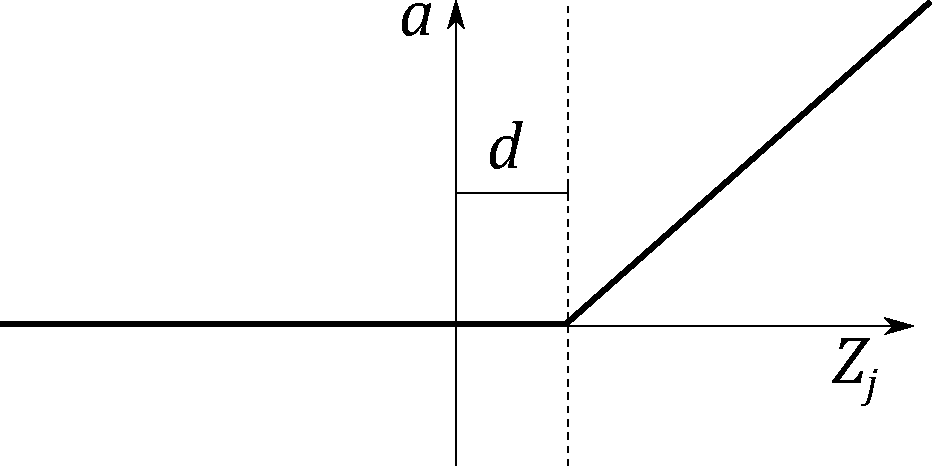
\includegraphics[width=0.5\linewidth]{images/relu.pdf}    

%     \caption{In figure captions, explain what the reader is looking at: ``A schematic of the rectifying linear unit, where $a$ is the output amplitude,
%     $d$ is a configurable dead-zone, and $Z_j$ is the input signal'', as well as why the reader is looking at this: 
%     ``It is notable that there is no activation \emph{at all} below 0, which explains our initial results.'' 
%     \textbf{Use vector image formats (.pdf) where possible}. Size figures appropriately, and do not make them over-large or too small to read.
%     }

%     % use the notation fig:name to cross reference a figure
%     \label{fig:relu} 
% \end{figure}


% \begin{figure}[h] 
%     \centering
%     \begin{subfigure}[b]{0.45\textwidth}
%         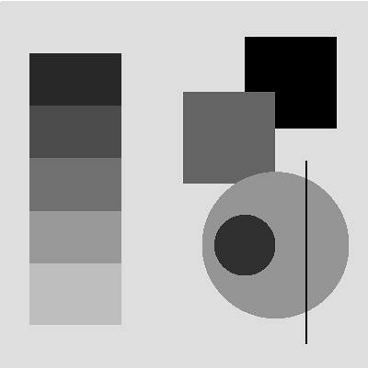
\includegraphics[width=\textwidth]{images/synthetic.png}
%         \caption{Synthetic image, black on white.}
%         \label{fig:syn1}
%     \end{subfigure}
%     ~ %add desired spacing between images, e. g. ~, \quad, \qquad, \hfill etc. 
%       %(or a blank line to force the subfigure onto a new line)
%     \begin{subfigure}[b]{0.45\textwidth}
%         
\includegraphics[width=\textwidth]{images/synthetic_2.png}
%         \caption{Synthetic image, white on black.}
%         \label{fig:syn2}
%     \end{subfigure}
%     ~ %add desired spacing between images, e. g. ~, \quad, \qquad, \hfill etc. 
%     %(or a blank line to force the subfigure onto a new line)    
%     \caption{Synthetic test images for edge detection algorithms. \subref{fig:syn1} shows various gray levels that require an adaptive algorithm. \subref{fig:syn2}
%     shows more challenging edge detection tests that have crossing lines. Fusing these into full segments typically requires algorithms like the Hough transform.
%     This is an example of using subfigures, with \texttt{subref}s in the caption.
%     }\label{fig:synthetic}
% \end{figure}

% \clearpage

% \subsection{Equations}

% Equations should be typeset correctly and precisely. Make sure you get parenthesis sizing correct, and punctuate equations correctly 
% (the comma is important and goes \textit{inside} the equation block). Explain any symbols used clearly if not defined earlier. 

% For example, we might define:
% \begin{equation}
%     \hat{f}(\xi) = \frac{1}{2}\left[ \int_{-\infty}^{\infty} f(x) e^{2\pi i x \xi} \right],
% \end{equation}    
% where $\hat{f}(\xi)$ is the Fourier transform of the time domain signal $f(x)$.

% \subsection{Algorithms}
% Algorithms can be set using \texttt{algorithm2e}, as in Algorithm \ref{alg:metropolis}.

% % NOTE: line ends are denoted by \; in algorithm2e
% \begin{algorithm}
%     \DontPrintSemicolon
%     \KwData{$f_X(x)$, a probability density function returing the density at $x$.\; $\sigma$ a standard deviation specifying the spread of the proposal distribution.\;
%     $x_0$, an initial starting condition.}
%     \KwResult{$s=[x_1, x_2, \dots, x_n]$, $n$ samples approximately drawn from a distribution with PDF $f_X(x)$.}
%     \Begin{
%         $s \longleftarrow []$\;
%         $p \longleftarrow f_X(x)$\;
%         $i \longleftarrow 0$\;
%         \While{$i < n$}
%         {
%             $x^\prime \longleftarrow \mathcal{N}(x, \sigma^2)$\;
%             $p^\prime \longleftarrow f_X(x^\prime)$\;
%             $a \longleftarrow \frac{p^\prime}{p}$\;
%             $r \longleftarrow U(0,1)$\;
%             \If{$r<a$}
%             {
%                 $x \longleftarrow x^\prime$\;
%                 $p \longleftarrow f_X(x)$\;
%                 $i \longleftarrow i+1$\;
%                 append $x$ to $s$\;
%             }
%         }
%     }
    
% \caption{The Metropolis-Hastings MCMC algorithm for drawing samples from arbitrary probability distributions, 
% specialised for normal proposal distributions $q(x^\prime|x) = \mathcal{N}(x, \sigma^2)$. The symmetry of the normal distribution means the acceptance rule takes the simplified form.}\label{alg:metropolis}
% \end{algorithm}

% \subsection{Tables}

% If you need to include tables, like Table \ref{tab:operators}, use a tool like https://www.tablesgenerator.com/ to generate the table as it is
% extremely tedious otherwise. 

% \begin{table}[]
%     \caption{The standard table of operators in Python, along with their functional equivalents from the \texttt{operator} package. Note that table
%     captions go above the table, not below. Do not add additional rules/lines to tables. }\label{tab:operators}
%     %\tt 
%     \rowcolors{2}{}{gray!3}
%     \begin{tabular}{@{}lll@{}}
%     %\toprule
%     \textbf{Operation}    & \textbf{Syntax}                & \textbf{Function}                            \\ %\midrule % optional rule for header
%     Addition              & \texttt{a + b}                          & \texttt{add(a, b)}                                    \\
%     Concatenation         & \texttt{seq1 + seq2}                    & \texttt{concat(seq1, seq2)}                           \\
%     Containment Test      & \texttt{obj in seq}                     & \texttt{contains(seq, obj)}                           \\
%     Division              & \texttt{a / b}                          & \texttt{div(a, b) }  \\
%     Division              & \texttt{a / b}                          & \texttt{truediv(a, b) } \\
%     Division              & \texttt{a // b}                         & \texttt{floordiv(a, b)}                               \\
%     Bitwise And           & \texttt{a \& b}                         & \texttt{and\_(a, b)}                                  \\
%     Bitwise Exclusive Or  & \texttt{a \textasciicircum b}           & \texttt{xor(a, b)}                                    \\
%     Bitwise Inversion     & \texttt{$\sim$a}                        & \texttt{invert(a)}                                    \\
%     Bitwise Or            & \texttt{a | b}                          & \texttt{or\_(a, b)}                                   \\
%     Exponentiation        & \texttt{a ** b}                         & \texttt{pow(a, b)}                                    \\
%     Identity              & \texttt{a is b}                         & \texttt{is\_(a, b)}                                   \\
%     Identity              & \texttt{a is not b}                     & \texttt{is\_not(a, b)}                                \\
%     Indexed Assignment    & \texttt{obj{[}k{]} = v}                 & \texttt{setitem(obj, k, v)}                           \\
%     Indexed Deletion      & \texttt{del obj{[}k{]}}                 & \texttt{delitem(obj, k)}                              \\
%     Indexing              & \texttt{obj{[}k{]}}                     & \texttt{getitem(obj, k)}                              \\
%     Left Shift            & \texttt{a \textless{}\textless b}       & \texttt{lshift(a, b)}                                 \\
%     Modulo                & \texttt{a \% b}                         & \texttt{mod(a, b)}                                    \\
%     Multiplication        & \texttt{a * b}                          & \texttt{mul(a, b)}                                    \\
%     Negation (Arithmetic) & \texttt{- a}                            & \texttt{neg(a)}                                       \\
%     Negation (Logical)    & \texttt{not a}                          & \texttt{not\_(a)}                                     \\
%     Positive              & \texttt{+ a}                            & \texttt{pos(a)}                                       \\
%     Right Shift           & \texttt{a \textgreater{}\textgreater b} & \texttt{rshift(a, b)}                                 \\
%     Sequence Repetition   & \texttt{seq * i}                        & \texttt{repeat(seq, i)}                               \\
%     Slice Assignment      & \texttt{seq{[}i:j{]} = values}          & \texttt{setitem(seq, slice(i, j), values)}            \\
%     Slice Deletion        & \texttt{del seq{[}i:j{]}}               & \texttt{delitem(seq, slice(i, j))}                    \\
%     Slicing               & \texttt{seq{[}i:j{]}}                   & \texttt{getitem(seq, slice(i, j))}                    \\
%     String Formatting     & \texttt{s \% obj}                       & \texttt{mod(s, obj)}                                  \\
%     Subtraction           & \texttt{a - b}                          & \texttt{sub(a, b)}                                    \\
%     Truth Test            & \texttt{obj}                            & \texttt{truth(obj)}                                   \\
%     Ordering              & \texttt{a \textless b}                  & \texttt{lt(a, b)}                                     \\
%     Ordering              & \texttt{a \textless{}= b}               & \texttt{le(a, b)}                                     \\
%     % \bottomrule
%     \end{tabular}
%     \end{table}
% \subsection{Code}

% Avoid putting large blocks of code in the report (more than a page in one block, for example). Use syntax highlighting if possible, as in Listing \ref{lst:callahan}.

% \begin{lstlisting}[language=python, float, caption={The algorithm for packing the $3\times 3$ outer-totalistic binary CA successor rule into a 
%     $16\times 16\times 16\times 16$ 4 bit lookup table, running an equivalent, notionally 16-state $2\times 2$ CA.}, label=lst:callahan]
%     def create_callahan_table(rule="b3s23"):
%         """Generate the lookup table for the cells."""        
%         s_table = np.zeros((16, 16, 16, 16), dtype=np.uint8)
%         birth, survive = parse_rule(rule)

%         # generate all 16 bit strings
%         for iv in range(65536):
%             bv = [(iv >> z) & 1 for z in range(16)]
%             a, b, c, d, e, f, g, h, i, j, k, l, m, n, o, p = bv

%             # compute next state of the inner 2x2
%             nw = apply_rule(f, a, b, c, e, g, i, j, k)
%             ne = apply_rule(g, b, c, d, f, h, j, k, l)
%             sw = apply_rule(j, e, f, g, i, k, m, n, o)
%             se = apply_rule(k, f, g, h, j, l, n, o, p)

%             # compute the index of this 4x4
%             nw_code = a | (b << 1) | (e << 2) | (f << 3)
%             ne_code = c | (d << 1) | (g << 2) | (h << 3)
%             sw_code = i | (j << 1) | (m << 2) | (n << 3)
%             se_code = k | (l << 1) | (o << 2) | (p << 3)

%             # compute the state for the 2x2
%             next_code = nw | (ne << 1) | (sw << 2) | (se << 3)

%             # get the 4x4 index, and write into the table
%             s_table[nw_code, ne_code, sw_code, se_code] = next_code

%         return s_table

% \end{lstlisting}

%==================================================================================================================================

\chapter{Evaluation} 
% How good is your solution? How well did you solve the general problem, and what evidence do you have to support that?

In this chapter, we shall outline the evaluation process and discuss results. First, we shall examine how evaluation was undertaken, including details on our experiments and user survey. Then, we shall show the results from both these evaluations. Finally, we shall discuss these results and present an argument based on the evidence garnered.

\section{Experiments Design}

Our experiments to gather quantitative (and some qualitative) data shall be undertaken on a simulated network; this shall be built using Mininet on a Ubuntu virtual machine. These experiments shall be conducted on all of our builds. 

For our WebTransport experiments, our network topology consists of two hosts, two switches and a server - this is illustrated by Figure \ref{perfect-topology-wt}.

\begin{figure}[h]
    \centering
    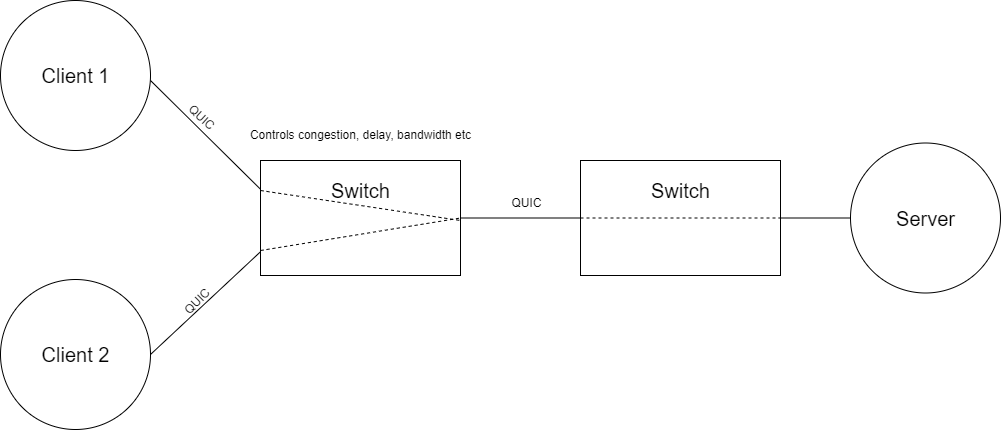
\includegraphics[width=0.8\columnwidth]{images/perfect-topology.png}
	\caption{A "perfect" network topology used to test our WebTransport builds.}
    \label{perfect-topology-wt}
\end{figure}

We can consider this network topology to be "perfect" as it has no competing traffic and therefore theoretically no congestion in the switches between nodes. This is not ideal for replicating realistic network conditions - however, as our WebTransport builds are likely to have varying performance in even perfect conditions, we can still effectively evaluate the builds in this perfect environment. We would suggest that further work could be done here to evaluate the WebTransport builds in a non-perfect simulated network, but due to time constraints we shall not do so in this project.

For our WebRTC experiments, our network topology shall consist of two hosts directly, one switch and two servers. We have one server that hosts PeerJS, and one that hosts socket.io. This topology is illustrated by Figure \ref{perfect-topology-webrtc}.

\begin{figure}[h]
    \centering
    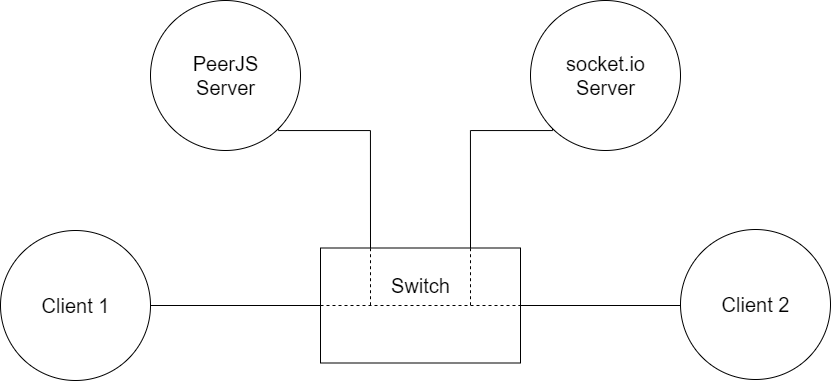
\includegraphics[width=0.7\columnwidth]{images/p2p-topology.png}
	\caption{A "perfect" network topology used to test our WebRTC builds.}
    \label{perfect-topology-webrtc}
\end{figure}

This topology has the same issue as our WebTransport topology in that it's "perfect". However, as we need to compare our WebRTC build to our WebTransport build, we must do so in the same network conditions to ensure the soundness of our experiments, so we shall continue to use these perfect conditions. Additionally, we shall disable audio data in our WebRTC build for the same reason.

Once these topologies have been built, we can experiment on our builds. The method is similar for both the WebTransport and WebRTC builds, with some slight variation to account for the different technologies. 

For our WebTransport builds, we first introduce lists of independent variables we wish to alter. Then, the network topology is adjusted based on the first items in these lists of independent variables. Following this, we automate the transmission of data between our two clients by using Selenium and the Mininet Python API to launch two instances of Google Chrome. During these transmissions, we use alternate builds that natively log relevant data and terminate once an arbitrary amount of packets (we send 1000 packets) has been sent. After these packets have been sent by the second client, the connection closes and relevant data is printed from our clients to Chrome's console log - this output is then fed into a CSV file and parsed. Then, the Mininet topology is shut down and the process repeats for the next set of independent variable values. Once the independent variable lists have been exhausted,  the outputted CSV data is analysed and, if necessary, parsed by matplotlib to generate visualisations that allow us to draw conclusions. 

The experiments for our WebRTC builds work very similarly, with some slight differences relating to the collection of relevant data and the Selenium automation of our clients. Instead of manually calculating the desired dependent variables from within our clients, we utilise the WebRTC Statistics API \cite{webrtc-stats-api}. From this API, we utilise the \textit{RTCInboundRtpStreamStats} dictionary \cite{webrtc-stats-api-inboundrtpstats}, and specifically the following measurement metrics: \textit{totalDecodeTime}, \textit{framesDecoded}, \textit{framesReceived},
\textit{packetsReceived}, \textit{packetsLost}, \textit{framesReceived} and \textit{framesDropped}. These metrics are collected on one of the two clients and outputted as before. Because the WebRTC builds are more stable, we chose to send 10000 packets rather than 1000 in order to have a greater chance of catching the occurrence of anomalies. Important dependent variables such as decoding time and loss are not affected by this decision, as decoding time is an average value and loss is a percentage.

As our primary aim is to evaluate WebTransport, WebRTC and the underlying data transfer methods rather than QUIC, SRTP and HTTP/3, measurements take place exclusively at our client endpoints. There is no notion in our results of how the data is transferred via the transport protocols. We had attempted to include some evaluations of QUIC for argument's sake, but ran into several difficulties. Our main issue was due to the way QUIC encrypts as much data as possible - it was not possible to extract meaningful data from packets sent between nodes as it was all encrypted. One solution to this may have been utilising qvis and qlog; these are tools specifically developed to work around this issue. However, qvis and qlog are in early stages of development and documentation is sparse - after attempting to get it to work, we decided to drop this aspect of experimentation and focus solely on WebTransport and WebRTC. In future work, it may be interesting to evaluate QUIC as well as WebTransport (and by extension, SRTP as well as WebRTC) and see if the API hinders or aids the transport protocol's performance in any way.

We shall now outline each of the performed experiments, highlighting independent and dependent variables, aims and expected results of each. The following experiments shall be conducted on all of our builds.

\subsection{The Experiments}

In total, we conducted five experiments on our WebTransport and WebRTC builds. In the following experiment descriptions, there are several definitions we must define. "Perceived latency" shall refer to how long it takes a frame to be fully processed by a client after the first packet of that frame is sent from the other client. "Actual latency" refers to how long it takes for a packet to be received by a client after being sent from the other client. "Decoding time" refers to the time difference between perceived latency and actual latency - this shall demonstrate how long it takes the receiving client to process a frame after the first packet of that frame is received. It should be noted that actual and perceived latency shall not be measured in our WebRTC builds. This is because it is not possible via the WebRTC Statistics API and we cannot develop an alternative solution within the timescale of our project - we can instead measure decoding time by dividing the amount of frames decoded by the total amount of frames received (both of these metrics are measured by the WebRTC Statistics API).

The dependent variables measured in each experiment are the same: perceived latency, actual latency, decoding time, packet loss (not measured in our WebTransport Streams build) and image quality. We chose these variables as we identified that these metrics are the most affected by adverse network conditions and also the most important to the end user experience. If any of these metrics are too high, the builds are likely suffering significantly and the user experience is probably degraded.  Although image quality is qualitative and therefore less precise, it is still a useful metric as it gives a simple indication of how the user experience is being affected.

The experiments are as follows.
\hfill{}\\
\subsubsection*{Bandwidth}
\hfill{}\\
Here, the independent variable is the bandwidth of the topology links. This experiment is important as it allows us to observe specifically how our builds cope with varying bandwidth. 
The expectation from this experiment is that, for all builds, both latencies worsen as bandwidth decreases, but packet loss will stay either the same or improve. We expect this effect to be particularly significant on the WebTransport Datagrams build where decreased bandwidth would result in there being more time for the client queue to accept late datagrams.
\hfill{}\\
\subsubsection*{Loss}
\hfill{}\\
Here, the independent variable is the loss percentage of the topology links. We expect that as it gets to extreme packet loss, both WebTransport builds will suffer extensively. In particular, the Datagrams build will output extremely poor image quality as we do not expect the code that deals with packet loss to operate well. We do not expect the Streams build to suffer in terms of image quality as streams are lossless, but latency may increase significantly as data is retransmitted more than usual. We expect that WebRTC will suffer slightly, but maintain decent image quality thanks to its forward error correction mechanisms.
\hfill{}\\
\subsubsection*{Latency}
\hfill{}\\
Here, the independent variable is the latency of the topology links. The aim of this experiment is to find out where WebTransport's bottleneck is - it will be interesting to see at what point the latency is too large for the packet reordering code to fall apart and discard too many packets. We do not expect the WebTransport Datagrams builds to cope well as latency increases. We expect that the Streams build and the WebRTC build will cope with respect to image quality, but the delay will be significant enough to degrade user experience.
\hfill{}\\
\subsubsection*{Network Quality (Bandwidth, Loss and Latency)}
\hfill{}\\
Here, the independent variables are the bandwidth, loss and latency of the topology links. The aim of this experiment is to simulate how WebTransport and WebRTC will perform on different qualities of network. We expect that the WebTransport builds will perform extremely poorly in bad network conditions, whereas the WebRTC build will likely maintain decent quality. In particular, the WebTransport Datagrams build will suffer for the same reasons as outlined in the previous experiments, and the image quality will degrade significantly. Additionally, the Streams build's rendered images will have too high of a delay to provide a satisfactory user experience.
\hfill{}\\
\subsubsection*{CPU Usage}
\hfill{}\\
During early and informal experimentation, it was noticed that the builds, even on a simulated network with perfect metrics, did not perform as well on our virtual machine as on our computer's native OS. We suspected that our virtual machine's comparatively worse system resource allocations were throttling the performance of the builds. To investigate this, we use the CPU usage (as a percentage value) of each client host as our independent variable.

\hfill{}\\
All of these experiments will give us an overview of how WebTransport and WebRTC send, receive and process video data in different network conditions. Hopefully, they shall allow us to achieve our main goal for this project of quantitatively evaluating the performance of several builds of video conferencing application using different APIs and data transfer methods. 

\section{User Survey Design}

In order to achieve our secondary aim of answering whether or not using WebTransport makes any noticeable differences to the user experience or not, we shall undertake a user survey. The ethics approval form for this survey can be seen in Figures \ref{ethics-1} and \ref{ethics-2}. This survey shall show anonymous participants recordings of six different builds of our video conferencing application implementations. The participants shall not know what technologies or data transfer methods are utilised in each build. The first three builds are our WebTransport Datagrams, WebTransport Streams and WebRTC builds - these are all run on our native machine in a "perfect" network (i.e. no adjusted metrics). The latter three builds are the same, but shall be running on our virtual machine with latency, bandwidth and loss adjusted. In these latter cases, the topology links shall have bandwidth set to 90 Mbps (Megabits per second), loss set to 0.5\% and latency set to 12.5 ms (milliseconds); these figures were arbitrarily chosen, but were shown to output a realistic simulation in our experiments.

Participants shall be asked three questions for each recording presented to them. For each question, the user is prompted to answer on a five-point Likert scale. These questions are as follows:

\textbf{\textit{"How would you rate the image quality of the video you are receiving? Does the received video resemble the video being sent out?"}}

\textbf{\textit{"How would you rate the "smoothness" of the video you are receiving? i.e. does it stutter or lag?"}}

\textbf{\textit{"Overall, how would you rate the video you are receiving out of 5?"}}

After answering these questions for each build, the user shall be presented a recording of all six builds on one screen. They shall then be asked to rank all the builds from best to worst, with no builds both being tied for one place.

Finally, the participant shall be give an opportunity to provide any feedback or observations they make.

Receiving these answers shall give us a good indication of whether or not users can tell the difference between our different builds and utilised technologies. Furthermore, it may provide some supplementary evidence (in addition to our experiments) of how each build performs.

\section{Evidence}
In the following section, we shall go through each experiment and discuss the results before discussing the results from our user surveys.

\subsection{Experiments}

\subsubsection{Experiment 1 - Adjusting Bandwidth} 
\hfill{} \\
Table \ref{tab:wt-dg-bw} displays all the collected data during this experiment for the WebTransport Datagrams build. From this data, we can generate several visualisations to aid us in understanding how the WebTransport Datagrams build handles received datagrams.
An interesting observation to make here is that the latencies and decoding time are relatively stable until link bandwidth gets below a certain threshold - here, it increases significantly. These effects can be seen in Figure \ref{fig:dg-bw-lat} and Figure \ref{fig:all-bw-decoding}. 

\begin{figure}[h]
    \centering
    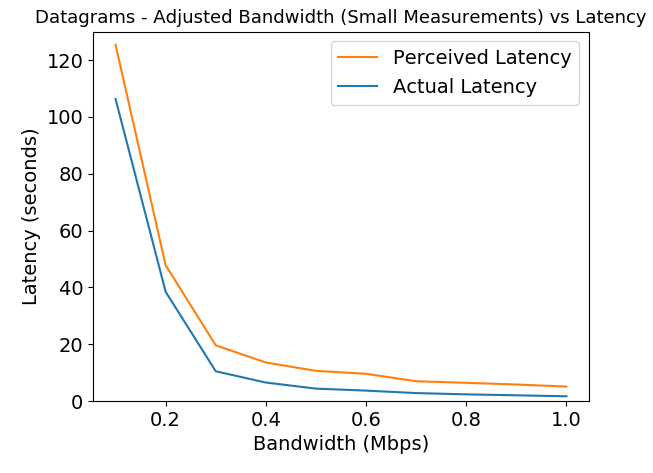
\includegraphics[width=0.52\linewidth]{images/bandwidth/dg-bw-lat-small.png}    
    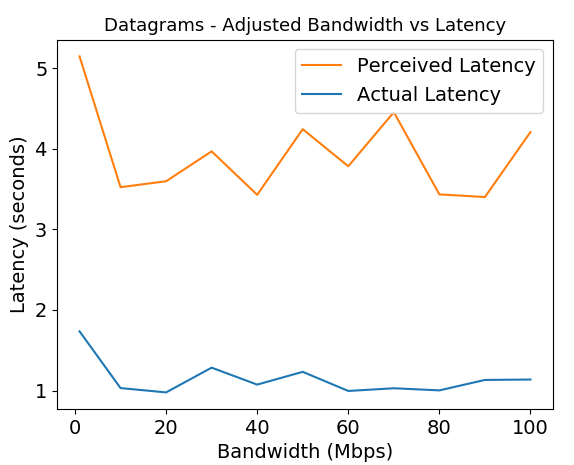
\includegraphics[width=0.46\linewidth]{images/bandwidth/dg-bw-lat.png}    
    \caption{Latencies affected by link bandwidth in the WebTransport Datagrams build.}

    % use the notation fig:name to cross reference a figure
    \label{fig:dg-bw-lat} 
\end{figure}

Throughout all our Datagrams build measurements, we can see that the perceived latency is consistently around 2-4 seconds more than the actual latency (indicating that it takes around this time to decode each frame of video data). Perceived latency (and as a result, our decoding time) is so high because our algorithms that handle packet loss and disorder are very inefficient - packets that arrive too early and are queued for significant periods of time greatly increase perceived latency and therefore decoding time. As latencies increase, the rendered output increasingly lags and image quality becomes very erratic. This same effect can be seen in our Streams build, although to less of an extent.

Table \ref{tab:wt-streams-bw} displays the results from our Streams build - loss is not measured here as streams are lossless. Figure \ref{fig:dg-streams-bw-lat} maps the Streams build's actual and perceived latencies onto the same plot as the Datagram build's. We can see that our Streams build largely follows the same trends as our Datagrams build, albeit with two significant differences. We can notice that the actual latency and perceived latency are much closer together, indicating that the decoding time of our Streams build is always far less than our Datagrams build. This makes sense as our Streams build does not have to deal with disordered or lost packets, meaning that frames can be decoded far quicker as WebTransport is able to process each packet as soon as it is received by the API. The second difference is the suddenly large latency values at the 1 Mbps mark. However, this is expected behaviour. This occurs because this threshold is the point at which the link bandwidth is smaller than the bandwidth at which our video is encoded at. To elaborate, our clients send video data of frame size 100 pixels x 100 pixels. Each pixel is equal to 1 byte, and so the total bytes it takes to transmit one frame is 10000 bytes (100 x 100). As our packets are 1024 bytes long and contain 1004 bytes of image data, it takes 10 packets to send one frame of video data (10000 ÷ 1004 = 9.96 i.e. 10 packets required). Our clients send roughly 10 frames per second, with packets constantly being sent, or "in flight". 10 frames per second means that roughly 100 packets are being sent every second, which means that approximately 102400 bytes (100 packets x packet size) are being transmitted at any one time. As we drop below the bandwidth threshold, our latencies (and consequently our decoding time) suffer as the bandwidth is often no longer able to account for the amount of packets constantly in flight.
The different thresholds for each build can be observed in Figure \ref{fig:dg-streams-bw-lat}. For our Streams build, the threshold is clearly 1 Mbps - 1 Mbps is equal to 125000 bytes, and it is feasible that packet retransmission results in this build's amount of data in flight crossing this threshold and suffering as a result. For our Datagrams build, the decline in latencies and decoding time is more gradual, but the threshold appears to be between 0.8 and 1 Mbps.

\begin{figure}[h]
    \centering
    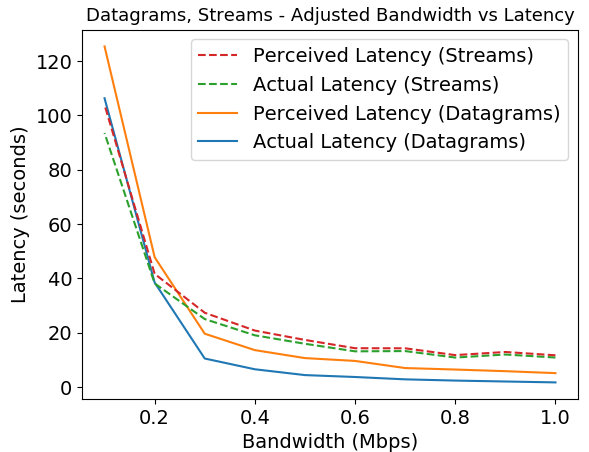
\includegraphics[width=0.49\linewidth]{images/bandwidth/dg-streams-bw-lat-small.png}  
    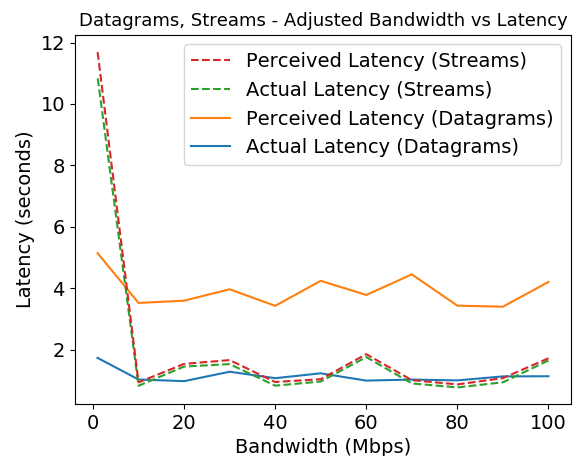
\includegraphics[width=0.49\linewidth]{images/bandwidth/dg-streams-bw-lat.png}    
    \caption{Latencies affected by link bandwidth in the WebTransport Datagrams and Streams builds.}

    % use the notation fig:name to cross reference a figure
    \label{fig:dg-streams-bw-lat} 
\end{figure}

Finally with our WebTransport builds, we can see that adjusting bandwidth does not affect application packet loss that much until we get to the same aforementioned threshold of 1 Mbps. This is displayed in Figure \ref{fig:dg-bw-loss}. This is once again, expected behaviour. The loss here is relatively insignificant, until we get to extremely low bandwidth values (between 0.1 and 0.2 Mbps).

\begin{figure}[h]
    \centering
     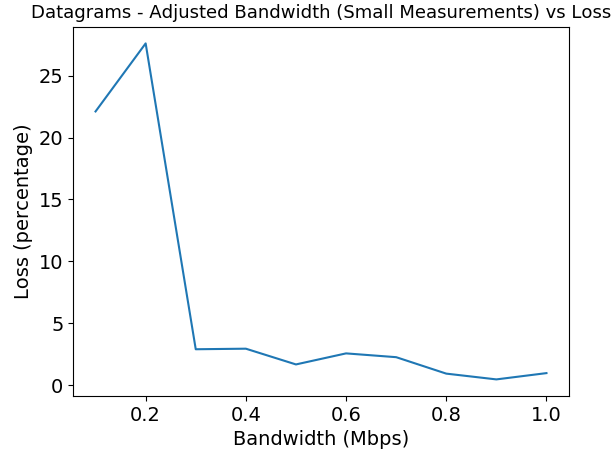
\includegraphics[width=0.49\linewidth]{images/bandwidth/dg-bw-loss-small.png}    
    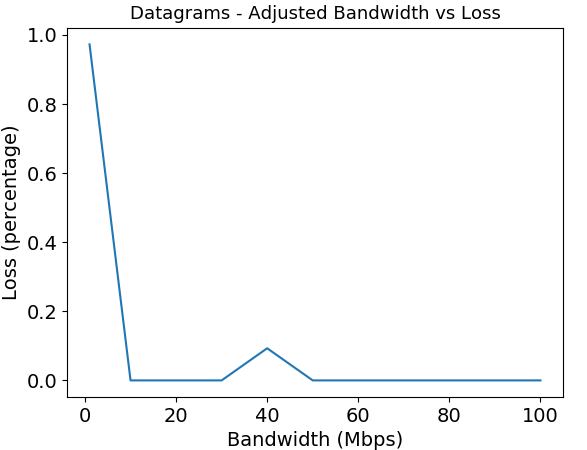
\includegraphics[width=0.49\linewidth]{images/bandwidth/dg-bw-loss.png}    
    \caption{Packet loss affected by link bandwidth in the WebTransport Datagrams and Streams builds.}

    % use the notation fig:name to cross reference a figure
    \label{fig:dg-bw-loss} 
\end{figure}

Our WebRTC builds generally fared better with respect to both decoding time and packet loss. All data gathered for this experiment can be seen in Table \ref{tab:webrtc-bw}.

We can clearly see that link bandwidth has no apparent effect on the WebRTC build. Decoding time varies slightly in apparently random fashion and frames are occasionally dropped, but there is again no discernible trend for this. Furthermore, the decoding time is far lower than our WebTransport Datagrams build, and lower than our WebTransport Streams build (particularly with extremely low bandwidth values) - this is displayed in Figure \ref{fig:all-bw-decoding}.

\begin{figure}[h]
    \centering
    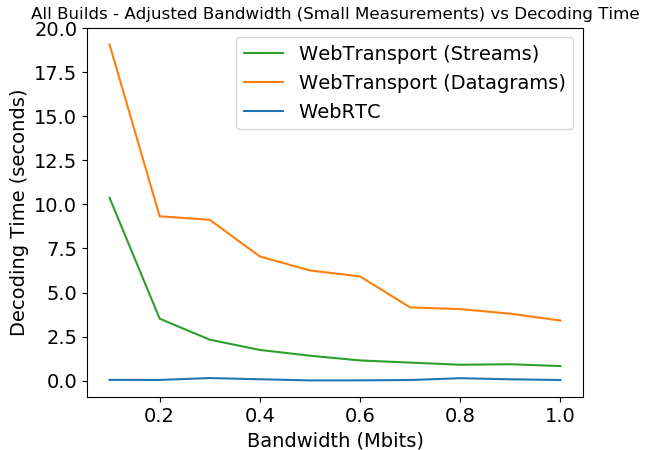
\includegraphics[width=0.51\linewidth]{images/bandwidth/all-bw-decoding-small.png}    
    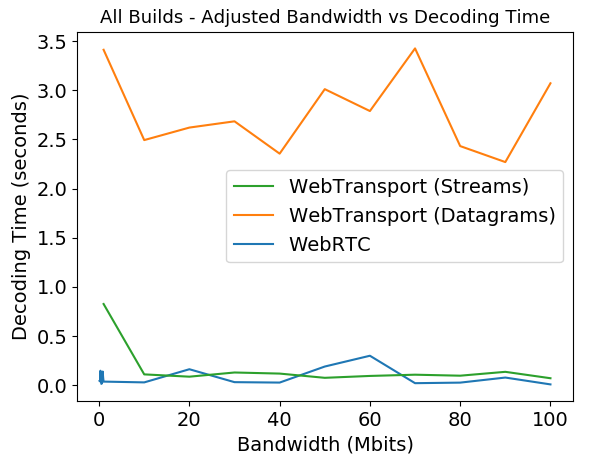
\includegraphics[width=0.48\linewidth]{images/bandwidth/all-bw-decoding.png}    
    \caption{Decoding time affected by link bandwidth in all our builds.}

    % use the notation fig:name to cross reference a figure
    \label{fig:all-bw-decoding} 
\end{figure}

Overall, it is clear to see that adjusting link bandwidth has a significant effect on our WebTransport builds' actual and perceived latencies, particularly as bandwidth values get to extreme lows. Our Streams build appears to perform slightly better than our Datagrams build in this regard, but suffers slightly sooner due to the higher amount of packets constantly in flight. Link bandwidth does not appear to affect loss in our Datagrams build that much until it gets to extreme lows between 0.1 and 0.2 Mbps. The WebRTC build handles low bandwidth extremely well, suffering very little packet loss and frame discards, and maintaining a steadily low decoding time. The WebRTC's build consistently low decoding time is likely what results in its consistently smooth video output - rendered video lags heavily when decoding time increases in our WebTransport builds.
\hfill{} \\

\subsubsection{Experiment 2 - Adjusting Latency} 
\hfill{} \\
The results from our WebTransport Datagrams build (as seen in Table \ref{tab:wt-dg-lat}) show some fairly predictable trends when increasing link latency. 
Firstly, both latencies steadily increase alongside link latency and appear to plateau between 12-16 seconds after the 100ms link latency point. There is a roughly two second decoding time throughout our measurements. This is unsurprising as, unlike the previous bandwidth experiments, the rate at which data is being received is not changed - this results in our build constantly receiving data, and therefore processing it at a constant rate. It should be noted that this experiment failed for our WebTransport Datagrams and Streams builds after 250ms, where the connection between the client and the server could no longer be established due to the server timing out. 
% \todo{insert how this is a QUIC policy}

Finally, we can see that the build performs very well in relation to packet loss until the 150ms link latency mark - here, after not losing any packets at all, we suddenly lose over half. This loss continues to increase as link latency increases; we can observe this on the left of Figure \ref{fig:dg-lat-loss-dg-streams-lat-lat}. As this sudden loss occurs, image quality sharply declines and rendered output becomes unrecognisable. It is unclear why this occurs at this specific point, but it demonstrates that the build does not handle high latency and resulting packet loss well. 

The application latencies of our WebTransport Streams build are similarly affected. The results of this experiment can be seen in Table \ref{tab:wt-streams-lat}. Decoding time is smaller than our Datagrams build until latency gets above 150ms - interestingly, the decoding time here becomes greater than our Datagrams counterpart. After this point, image quality and smoothness degrades. This high decoding time occurs due to the lossless nature of streams. As we know, if packets are lost in a streams connection, these packets are retransmitted. In this scenario, the decoding of our video frame would halt to wait for these retransmitted packets to arrive because streams deliver packets in order. In a low-latency network, this would negligibly increase decoding time - however, in high-latency networks, it takes longer for these packets to be retransmitted and decoding time consequently rises significantly. This is the main reason why streams are generally considered to be unsuitable for use in video conferencing applications. This conclusion is corroborated by Perkins' and Ott's 2018 paper that states a significant problem with QUIC's streams implementation is "media data being retransmitted once it has passed its play-out
deadline and is no longer needed" \cite{perkins2018}. 
The differences in actual and perceived latencies between the two builds can be seen on the right of Figure \ref{fig:dg-lat-loss-dg-streams-lat-lat}. From this, we can see that the Streams build is able to render video frames faster than the Datagrams build at low link latencies. However, as link latency increases and the Streams build's decoding time increases, the Datagrams build actually renders video frames faster. However, this is by a relatively slim margin (~2-4 seconds), and the image quality of both is very poor. 

% \begin{figure}[h]
%     \centering
%     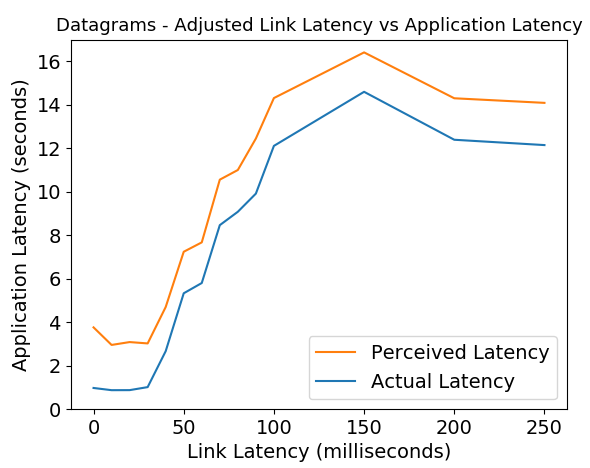
\includegraphics[width=0.49\linewidth]{images/latency/dg-lat-lat.png}
%     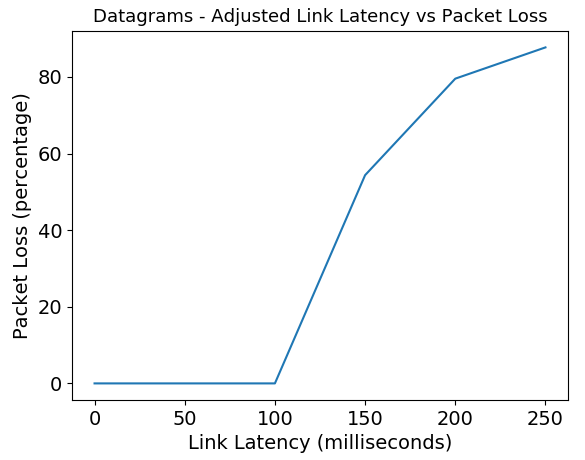
\includegraphics[width=0.49\linewidth]{images/latency/dg-lat-loss.png}
%     \caption{Left: Application latency affected by link latency in our WebTransport Datagrams build. Right: Packet loss affected by link latency in our WebTransport Datagrams build.}
%     % use the notation fig:name to cross reference a figure
%     \label{fig:dg-lat-lat-lat-loss} 
% \end{figure}

\begin{figure}[h]
    \centering
    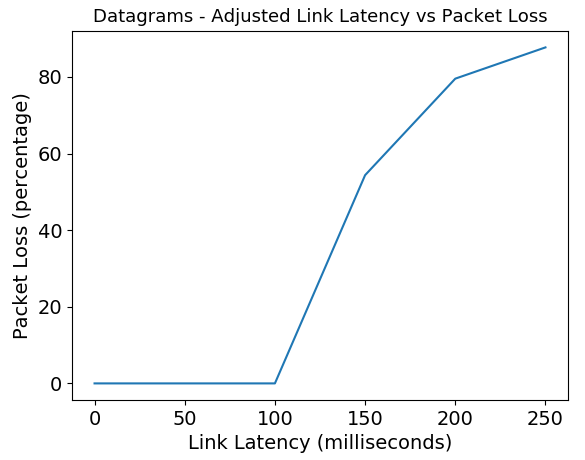
\includegraphics[width=0.475\linewidth]{images/latency/dg-lat-loss.png}
    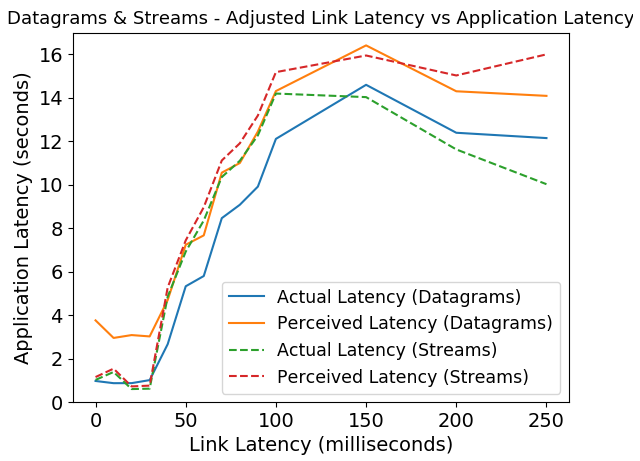
\includegraphics[width=0.515\linewidth]{images/latency/dg-streams-lat-lat.png}
    \caption{Left: Packet loss affected by link latency in our WebTransport Datagrams build. Right: Application latency affected by link latency in both WebTransport builds.}
    % use the notation fig:name to cross reference a figure
    \label{fig:dg-lat-loss-dg-streams-lat-lat} 
\end{figure}

WebRTC fared very well under high latency. As seen in Table \ref{tab:webrtc-lat}, there was no packet loss and there is no indication that decoding time was affected. Decoding time, once again, was very small. There was obviously a visible delay in the receiving video being displayed due to the link latency, but the image quality and smoothness were unaffected. A comparison of decoding time between all the builds can be seen in Figure \ref{fig:all-dec-lat}.

\begin{figure}[h]
    \centering
    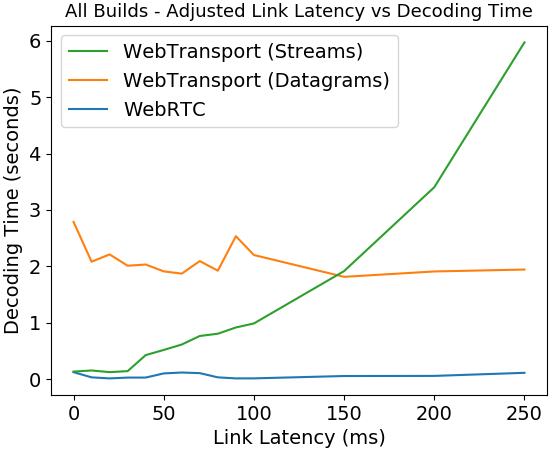
\includegraphics[width=0.6\linewidth]{images/latency/all-dec.png}
    \caption{All builds' decoding time against link latency mapped onto one graph.}
    % use the notation fig:name to cross reference a figure
    \label{fig:all-dec-lat} 
\end{figure}

Additionally, WebRTC does not suffer any packet loss even in high latency. However, the experiment failed after 500ms latency as the connection between the clients could no longer be established.

Overall, WebRTC greatly outperforms the WebTransport builds when adjusting latency. The Datagrams build is let down by its high decoding time and sensitivity to packet loss, and the Streams build suffers from comparatively high decoding times at high latencies. The WebRTC build maintains very low decoding time at all latencies and did not drop any packets during this experiment.
\hfill{} \\
\subsubsection{Experiment 3 - Adjusting Loss} 
\hfill{} \\
As seen in Table \ref{tab:wt-dg-loss}, our WebTransport Datagrams build results for this experiment were generally as expected. The build's packet loss percentage is usually approximately equal to the link loss multiplied by six - this is because we have six links in our network topology. This can be observed on the left of Figure \ref{fig:dg-loss-lat}. Because of this multiplication, experiments past 20\% link loss did not work as connection could not be established. 

% \begin{figure}[h]
%     \centering
%     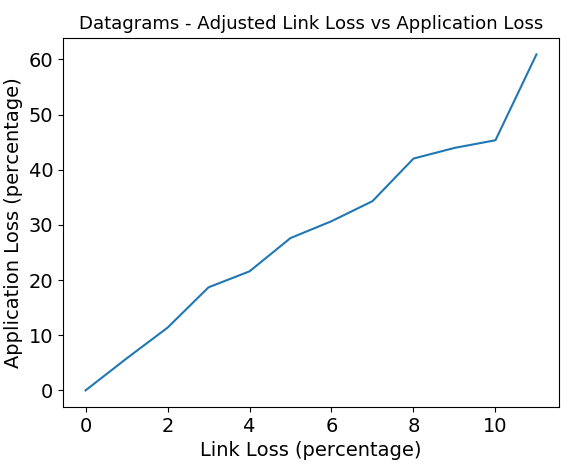
\includegraphics[width=0.6\linewidth]{images/loss/dg-loss-loss.png}
%     \caption{Adjusted link loss' effect on packet loss in our WebTransport Datagrams build.}
%     % use the notation fig:name to cross reference a figure
%     \label{fig:dg-loss-loss} 
% \end{figure}

As seen on the right in Figure \ref{fig:dg-loss-lat}, perceived latency is slightly lower than in our other experiments - this is because our packet handling mechanisms often discarded frames with heavy packet loss and rendered them as incomplete frames. Because of this, although the received video may have been relatively smooth, the image quality quickly became very poor. In general, the decoding time stays between approximately 2-3 seconds with some small outliers.

\begin{figure}[h]
    \centering
    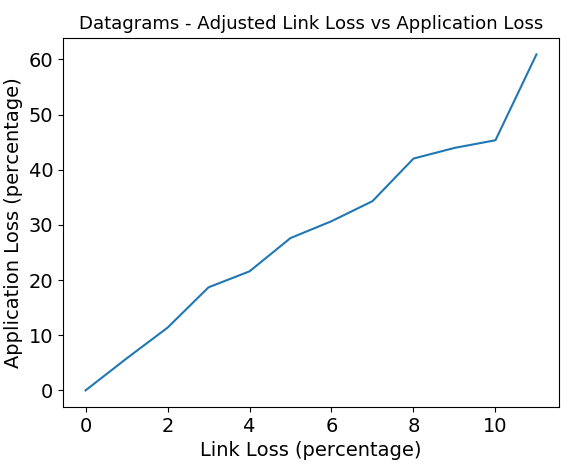
\includegraphics[width=0.49\linewidth]{images/loss/dg-loss-loss.png}
    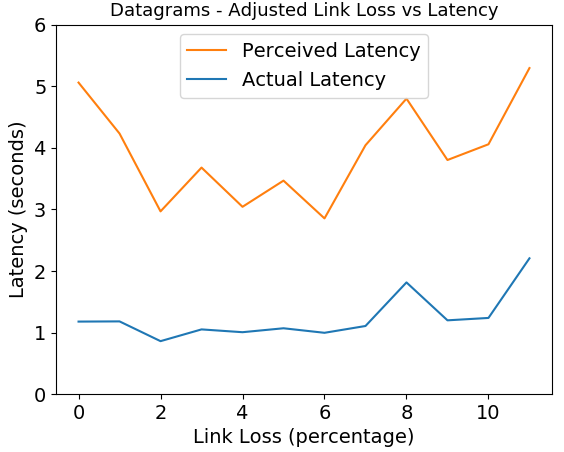
\includegraphics[width=0.49\linewidth]{images/loss/dg-loss-lat.png}
    \caption{Left: Adjusted link loss' effect on packet loss in our WebTransport Datagrams build. Right: Adjusted link loss' effect on latencies in our WebTransport Datagrams build.}
    % use the notation fig:name to cross reference a figure
    \label{fig:dg-loss-lat} 
\end{figure}

The results from the experiment on our Streams build can be seen in Table \ref{tab:wt-streams-loss}. As we can see, the experiments did not function past 12\% link loss rate here. This is surprising since streams are lossless, but it seems that the connection to the server timed out during connection establishment as packets were being retransmitted. Aside from this, results indicate that the Streams build functions adequately with high link loss rate. Decoding time does increase with loss rate - this is expected as the client must wait for packets to be retransmitted before completing a frame, and higher loss results in more retransmissions. Decoding time is relatively low, but still does rise alongside our link loss rate. This is once again because lost packets need to be retransmitted, thus stalling frame processing and increasing decoding time. However, as our links have very low latency, this does not have a significant effect on our decoding time as packets are quickly retransmitted. There is no solid discernible trend with our actual and perceived latencies - it does appear that with higher loss rates, we are more likely to see higher latencies, but there are too many outliers to state that there is a direct relationship between link loss rate, actual latency and perceived latency.

Our WebRTC build functioned well with high loss, as seen in Table \ref{tab:wrtc-loss}. Once again, these experiments were not able to progress past 20\% link loss rate as connection establishment failed. 
Surprisingly, the WebRTC build suffered no packet loss. This is because of WebRTC's forward error correction mechanisms. Indeed, more frames were dropped than usual in comparison to other WebRTC experiments, as they were likely "timed out" as packets were being retransmitted, but image quality and smoothness never appeared to decline or lag. Furthermore, decoding time once again stayed very consistent and appeared to be unaffected by link loss rate.

In the left of Figure \ref{fig:dg-nwq-loss}, we can see each build's decoding time mapped onto one graph.

% \begin{figure}[h]
%     \centering
%     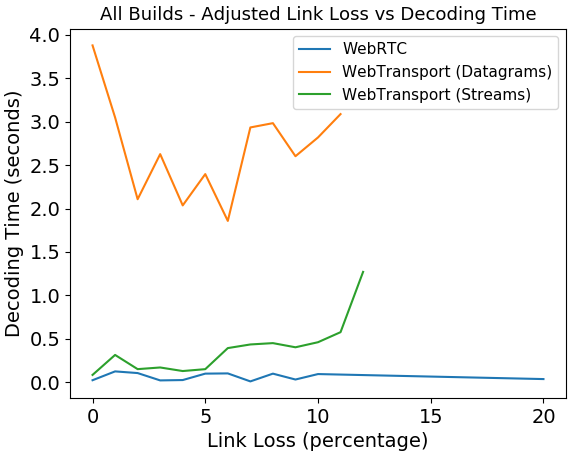
\includegraphics[width=0.6\linewidth]{images/loss/all-loss-decode.png}
%     \caption{All builds' decoding time against link loss rate mapped onto one graph.}
%     % use the notation fig:name to cross reference a figure
%     \label{fig:all-dec-loss} 
% \end{figure}

From this and our previous results, we can determine that our Datagrams build is by far the worst at dealing with loss. Our Streams build functions well at low loss rates but begins to suffer at higher loss rates, and WebRTC deals with loss extremely well.

\hfill{} \\
\subsubsection{Experiment 4 - Adjusting Network Quality (Bandwidth, Latency and Loss)} 
\hfill{} \\
In this experiment, all builds behave as expected. It should be noted that, as before, experiments only ran certain amounts of configuration numbers due to connection establishment issues: our Datagrams build ran 13, our Streams build ran 10 and our WebRTC build ran 20. The data for this experiment can be viewed in Table \ref{tab:wt-dg-nwq}. The most significant effects discovered in the previous experiments are exacerbated here by the other metrics in each configuration. For example, the Datagrams build's packet loss follows a similar pattern to the loss discovered in our Latency experiment (seen in the left of Figure \ref{fig:dg-lat-loss-dg-streams-lat-lat}), but it occurs at a far earlier latency. Instead of spiking at 150ms like before, the extreme packet loss occurs at a latency of 37.5ms (or independent variable Configuration 4); this is because of this configuration's corresponding link loss value of 1.5\% further worsening the existing packet loss. This effect can be seen in the right of Figure \ref{fig:dg-nwq-loss}.

\begin{figure}[h]
    \centering
    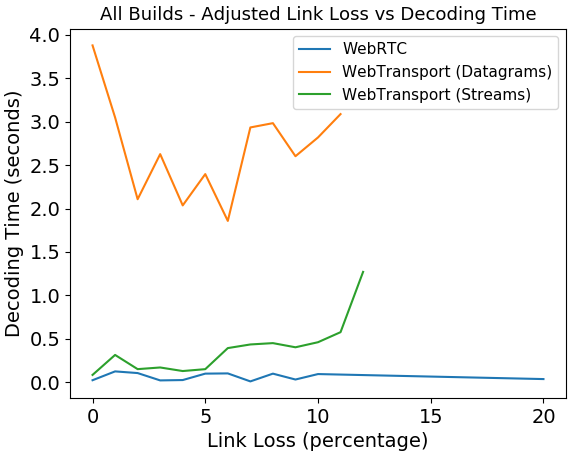
\includegraphics[width=0.49\linewidth]{images/loss/all-loss-decode.png}
    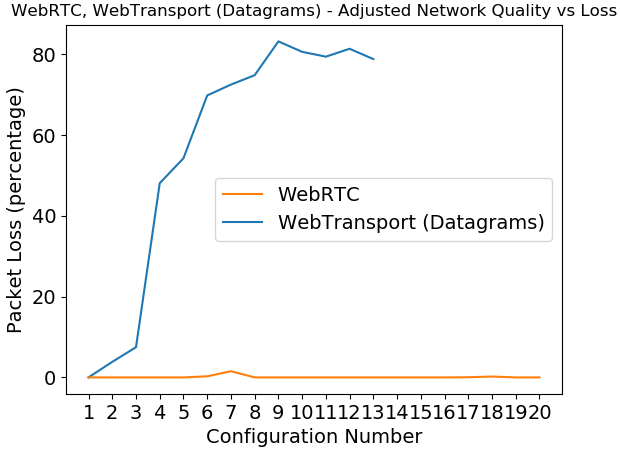
\includegraphics[width=0.49\linewidth]{images/combo/dg-nwq-loss.png}
    \caption{Left: All builds' decoding time against link loss rate mapped onto one graph. Right: The effect of our network quality configurations on WebTransport (Datagrams) and WebRTC builds' packet loss.}
    % use the notation fig:name to cross reference a figure
    \label{fig:dg-nwq-loss} 
\end{figure}

Another notable effect from previous experiments that is worsened here is latency's and loss' effects on our Streams build's decoding time. In our Latency experiment, the Streams build's decoding time became worse than our Datagrams build's at a link latency of 150ms - this can be seen in Figure \ref{fig:all-dec-lat}. In this experiment, this same thing occurs at a link latency of 62.5ms (or at Configuration 6). This can be observed on the left in Figure \ref{fig:all-nwq-dec}. This happens due to the effect link latency has on the WebTransport Streams build's decoding time being combined with the effect link loss rate has on it - more packets are lost and so total retransmission time increases, thus increasing decoding time.

\begin{figure}[h]
    \centering
    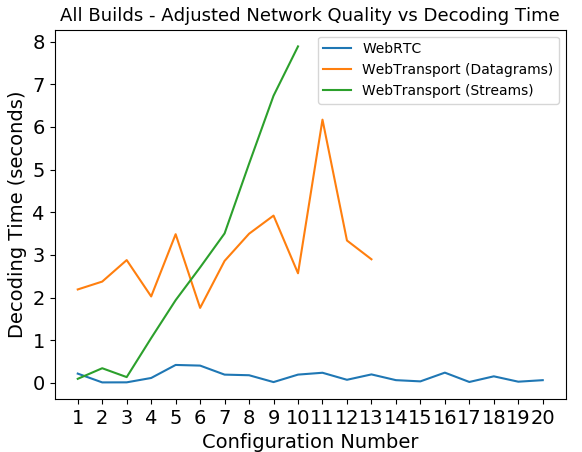
\includegraphics[width=0.49\linewidth]{images/combo/all-nwq-dec.png}
    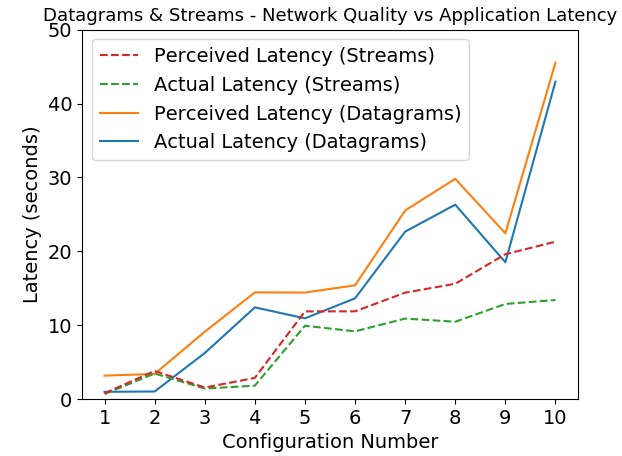
\includegraphics[width=0.49\linewidth]{images/combo/dg-streams-nwq-lat.png}
    \caption{Left: All builds’ decoding time against our adjusted network quality configurations mapped onto one graph. Right: Application latency affected by realistic network conditions in both WebTransport builds.}
    % use the notation fig:name to cross reference a figure
    \label{fig:all-nwq-dec} 
\end{figure}

Despite this poor decoding time, our Streams build still outperforms our Datagrams build due to the latter's previous issues with actual and perceived latencies reoccurring in this experiment. These two metrics are at the worst we have seen them by far, indicating that our Datagrams build does not perform well at all in realistic network conditions. This can be seen on the right in Figure \ref{fig:all-nwq-dec}.

% \begin{figure}[h]
%     \centering
%     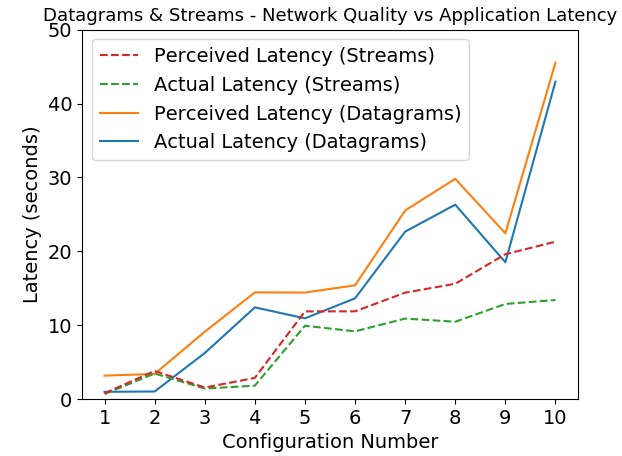
\includegraphics[width=0.6\linewidth]{images/combo/dg-streams-nwq-lat.png}
%     \caption{Application latency affected by realistic network conditions in both WebTransport builds.}
%     % use the notation fig:name to cross reference a figure
%     \label{fig:dg-streams-nwq-lat} 
% \end{figure}

Our WebRTC build performed well. As seen on the left in Figure \ref{fig:all-nwq-dec}, it once again maintained a very good decoding time throughout the experiment, resulting in high quality and smooth video playback. One interesting thing to note is that this experiment was the only one in which we noticed some packet loss (seen in the right of Figure \ref{fig:dg-nwq-loss}) - however, the amount of packets lost is relatively minuscule and there was no perceivable effect on image quality or smoothness. 

The main conclusion from this experiment is that all of the negative effects due to individual metrics observed in our previous experiments are exacerbated when combined into one simulated network. Our WebRTC build once again outperforms our WebTransport builds, and our Streams build generally outperforms its Datagrams counterpart. The Datagrams build suffers significantly in all configurations excluding the first one (where the network conditions are perfect), indicating that it does not perform well in realistic network conditions.

\hfill{} \\
\subsubsection{Experiment 5 - Adjusting CPU Usage} 
\hfill{} \\
Our WebTransport Datagrams build suffers a lot from varying CPU usage of the clients. Results for this can be seen in Table \ref{tab:wt-dg-cpu}. There are no apparent trends here, but it is evident to see that even dropping each client to using 90\% of available CPU resources causes our latencies and decoding time to increase significantly. Actual latency, perceived latency and our decoding times all vary significantly in seemingly random fashion. This indicates that our Datagrams build heavily relies on a powerful machine to render frames in a timely manner. Packet loss, however, does not appear to be significantly affected. Image quality and smoothness varies from good to unrecognisable. 

Our WebTransport Streams build handles varying CPU usage comparatively well. Results here can be seen in Table \ref{tab:wt-streams-cpu}. Similarly to previous experiments, actual and perceived latency increase as CPU usage gets to extremely low values, but not nearly to the same extent as our Datagrams build. We can see the latencies of our two WebTransport builds in Figure \ref{fig:dg-streams-cpu-lat}. Decoding time also increases slightly alongside the latencies, but is generally low enough to be adequate. In general, image quality and smoothness is good, but smoothness degrades with the extremely low CPU usage values.

\begin{figure}[h]
    \centering
    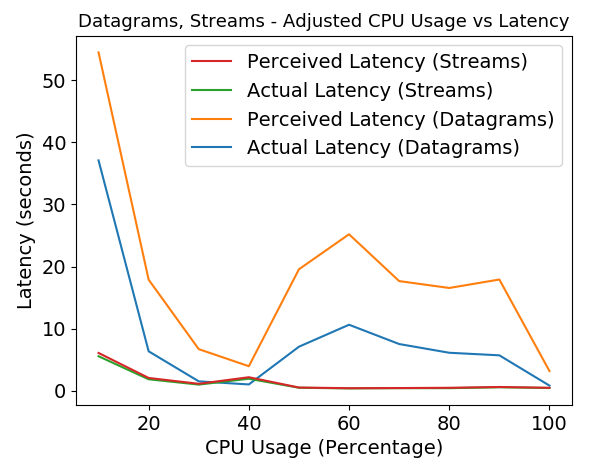
\includegraphics[width=0.6\linewidth]{images/cpu/dg-streams-cpu-lat.png}
    \caption{Application latencies affected by CPU usage in both WebTransport builds.}
    % use the notation fig:name to cross reference a figure
    \label{fig:dg-streams-cpu-lat} 
\end{figure}

The WebRTC build performed extremely well - CPU usage appears to have no effect on the build's performance in any regard. However, it should be noted that the WebRTC build failed to launch at 20\% and 10\% CPU usage, so we were unable to evaluate the metrics at these values. The results from this experiment can be seen in Table \ref{tab:wrtc-cpu}.

We can see the decoding time of all builds against CPU usage on the left in Figure \ref{fig:all-dec-cpu}, and just our Streams build against our WebRTC build on the right.

\begin{figure}[h]
    \centering
    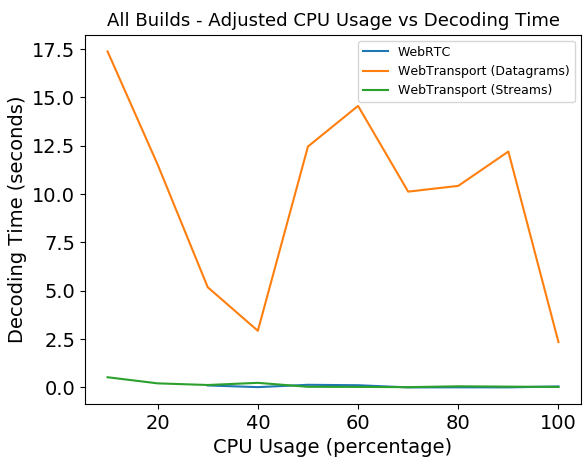
\includegraphics[width=0.49\linewidth]{images/cpu/all-cpu-decode.png}
    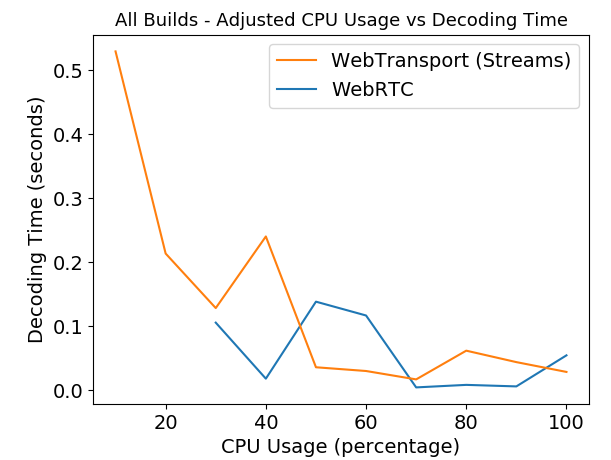
\includegraphics[width=0.49\linewidth]{images/cpu/wrtc-streams-cpu-decode.png}
    \caption{Left: builds' decoding time against CPU usage mapped onto one graph. Right: The WebTransport Streams and WebRTC builds' decoding time against CPU usage.}
    % use the notation fig:name to cross reference a figure
    \label{fig:all-dec-cpu} 
\end{figure}

As we can see on the left figure, our Datagrams build is clearly the worst-performing with regards to decoding time. On the right figure, we see that our Streams build and our WebRTC build perform similarly - any difference is negligible as the decoding time values are so small. Although WebRTC does appear to be slightly better, we cannot conclusively state this as we do not know what would have happened had the experiment run when CPU Usage was 10\% and 20\%.  

Overall, it is clear that our Datagrams build is heavily affected by varying CPU usage and would not perform well on less powerful devices; this is likely due to the inefficient algorithms that handle packet disorder and loss. Our Streams build is only slightly affected, and our WebRTC build does not appear to be affected at all (although this may not be the case in extremely low CPU usage percentages).

\hfill{} \\
\subsubsection{Overall Experiments Results} 
\hfill{} \\

Overall, it is clear that WebRTC outperforms both our WebTransport builds. Poor network quality barely affects it, and image quality and smoothness is almost always good. 

On the whole, our Streams build performs better than our Datagrams build. The Streams build does suffer in extremely poor network conditions, particularly when link latency and loss are high; such conditions result in long decoding times and video output that is not smooth. The build performs well in our good and average network conditions, but the image quality and smoothness is never as good as our WebRTC build simply because data transfer via streams is too slow.

Our Datagrams build has two main points of failure: the algorithms that handle packet loss and disorder, and the lack of mechanisms to negate packet loss in the first place. Evidence of the former is the results returned from our actual latencies, perceived latencies and decoding times. The reason that actual latency is high is that the client cannot start processing another frame until it has finished processing the current frame - when CPU usage or network conditions are poor, it takes far longer to process each frame and the perceived latency increases, consequently resulting in the perceived latency of the next frame to increase. The algorithms that handle packet disorder and loss are not robust at all and heavily rely on good network conditions and CPU usage. There are several ways that these algorithms could be improved; we would suggest utilising a more efficient data structure for the queues, dynamically varying the timeout for discarding frames and implementing some sort of multithreading functionality that continues to receive and process packets whilst our queue is being managed.
Evidence of poor loss management can be seen in the differences of packet loss statistics between our Datagrams and WebRTC builds. Despite both delivering packets in an unreliable fashion, WebRTC almost never loses packets, whereas our Datagrams build does so regularly. If we were to implement, for example, forward error correction mechanisms in our Datagrams build to the same standard as WebRTC's implementation, we may see heavily reduced packet loss which would in turn reduce the strain on our previously discussed packet handling algorithms.

Our Streams build performing better than its Datagrams counterpart was unexpected as datagrams' timely nature is theoretically better for video conferencing applications. However, the Streams build does not have much room for improvement - additional tweaks may slightly improve performance, but it is very unlikely that it is technically possible to be as good as WebRTC. However, as evidenced by these experiments, the Datagrams build does have a lot of room for improvement - we believe that it could theoretically outperform WebRTC due to WebTransport's support for developer freedom and utilisation of QUIC. If steps were taken to address the two main weaknesses outlined above, it would be interesting to reevaluate these builds and see if WebTransport could be used to its full potential.

These results prove that we have quantitatively evaluated the performance of several builds of a simple video conferencing application using different APIs (WebTransport and WebRTC) and data transfer methods, thus achieving the main goal of this project.
\hfill{} \\
\subsection{User Survey}
Our user survey generally backs up the findings from our experiments. For the survey, we gathered 25 anonymised participants from a range of ages and technical abilities.

In Table \ref{tab:likert-responses}, we can observe the average results of the responses to our Likert scale questions concerning the image quality, video smoothness and overall quality of each build. These Likert scale questions were from 1-5, with 1 being the lower end of the scale and 5 being the higher; we calculated the average result from each answer by totalling the responses (with a response of "4" for example being equal to 4 points) and dividing by 25 (the total number of participants). 

\begin{table}[H]
\centering
\resizebox{\textwidth}{!}{%
\begin{tabular}{lllll}
\hline
Build                                     & Avg. Quality & Avg. Smoothness & Avg. Overall &  \\ \hline
Alpha (WebTransport Datagrams)            & 2.52         & 1.12            & 1.76         &  \\
Beta (WebRTC)                             & 4.44         & 4.68            & 4.64         &  \\
Charlie (WebTransport Streams)            & 2.28         & 1.32            & 1.64         &  \\
Delta (WebTransport Datagrams  - Mininet) & 2            & 1.24            & 1.44         &  \\
Echo (WebRTC - Mininet)                   & 3.92         & 3.44            & 3.36         &  \\
Foxtrot (WebTransport Streams - Mininet)  & 2.44         & 1.56            & 1.84         &  \\ \hline
\end{tabular}%
}
\caption{Participant responses to our survey's Likert scale questions.}
\label{tab:likert-responses}
\end{table}

Before discussing these results, we shall display the outcome for our final question asking participants to rank each build. The following graph (Figure \ref{fig:ranks}) was generated by assigning points to each build depending on what ranks they were given by each participant - 1st place results in a build receiving 6 points, 2nd place results in a build receiving 5 points and so on. Every participant's ranking is taken into account, meaning that a build can have a potential total of 150 points (25 participants x 6 points if a build is given 1st place by each participant).  

\begin{figure}[h]
    \centering
    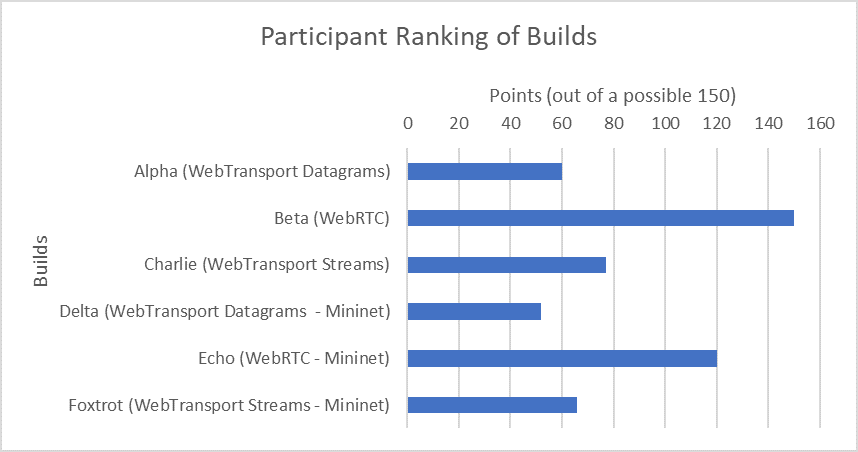
\includegraphics[width=0.73\linewidth]{images/user-survey-builds-rank.png}    

    \caption{Results calculated from participants' build rankings.}

    % use the notation fig:name to cross reference a figure
    \label{fig:ranks} 
\end{figure}

It is clear to see that our two WebRTC builds, Beta and Echo, proved to be the most well-received by our participants. In particular, participants unanimously responded that Beta was the highest-performing build across all metrics, with all participants ranking it as their highest build. Furthermore, Echo was second place in every question - this reflects our quantitative data that shows the WebRTC builds had generally better performance than the WebTransport ones.  

Our WebTransport builds had generally more mixed results, even when taking into account the "perfect" network conditions of Alpha and Charlie. Some of the results seem quite contradictory - for example, Foxtrot has a better average overall score than Charlie, but places worse in the final rankings. Additionally, Alpha has a better average overall score than Charlie, but once again places worse in the final rankings. This indicates that, in comparison to how the WebRTC builds scored and placed, there is less certainty about how the WebTransport builds perform with respect to each other. This is corroborated by feedback from four participants that stated it was difficult to tell the difference between the poorly-performing builds, as according to one participant, they were "just as bad as each other". Additionally, some participants stated that they were more certain of their answers when ranking the builds rather than when responding to the Likert scales - because of this, we have decided to assume that the final rankings are more indicative of apparent performance than the results from the Likert scale questions.

An important result to note is that participants were able to tell when network conditions affected quality - the three Mininet builds were each placed lower in the final rankings than their perfect network counterparts.

Finally, we can determine that, according to user observation, Streams builds perform better than Datagrams builds in both perfect network conditions and more realistic network conditions. This corroborates the data from our experiments.

From these results, we can clearly see that using different technologies and data transfer methods have a significant effect on the user experience. If we go by the final rankings, participants were successfully able to assess the quality of each build - this is evidenced by our experiment results (WebRTC being better than WebTransport, our Streams build being better than our Datagrams build) and by the fact that each Mininet build is ranked lower than their corresponding perfect network builds. A key question asked by this project was whether the extra development overhead of using WebTransport makes a difference to the user or not - it clearly does, although obviously not in the way we wanted as it has a negative effect. Had our WebTransport builds been of a closer quality to (or better than) our WebRTC builds, it would have been interesting to see if this distinction between the builds using the two APIs could still be made by end users, as this would perhaps indicate to us whether advocating for the continued development of WebTransport would even be worth it. However, as our WebTransport builds fall short in terms of performance, we feel that this particular question has not been answered by this project. We can, however, say that the extra development overhead was not worth it in this instance from a purely results-oriented standpoint, and the user responses in this survey confirmed that. Despite not answering the question presented in our secondary project aim, the user survey was still useful as it serves as further evidence of our experiment results. 


% \section{Guidance}
% \begin{itemize}
%     \item
%         Ask specific questions that address the general problem.
%     \item
%         Answer them with precise evidence (graphs, numbers, statistical
%         analysis, qualitative analysis).
%     \item
%         Be fair and be scientific.
%     \item
%         The key thing is to show that you know how to evaluate your work, not
%         that your work is the most amazing product ever.
% \end{itemize}

% \section{Evidence}
% Make sure you present your evidence well. Use appropriate visualisations, 
% reporting techniques and statistical analysis, as appropriate. The point is not
% to dump all the data you have but to present an argument well supported by evidence gathered.

% If you use numerical evidence, specify reasonable numbers of significant digits; don't state ``18.41141\% of users were successful'' if you only had 20 users. If you average \textit{anything}, present both a measure of central tendency (e.g. mean, median) \textit{and} a measure of spread (e.g. standard deviation, min/max, interquartile range).

% You can use \texttt{siunitx} to define units, space numbers neatly, and set the precision for the whole LaTeX document. 

% % setup siunitx to have two decimal places
% \sisetup{
% 	round-mode = places,
% 	round-precision = 2
% }

% For example, these numbers will appear with two decimal places: \num{3.141592}, \num{2.71828}, and this one will appear with reasonable spacing \num{1000000}.



% If you use statistical procedures, make sure you understand the process you are using,
% and that you check the required assumptions hold in your case. 

% If you visualise, follow the basic rules, as illustrated in Figure \ref{fig:boxplot}:
% \begin{itemize}
% \item Label everything correctly (axis, title, units).
% \item Caption thoroughly.
% \item Reference in text.
% \item \textbf{Include appropriate display of uncertainty (e.g. error bars, Box plot)}
% \item Minimize clutter.
% \end{itemize}

% See the file \texttt{guide\_to\_visualising.pdf} for further information and guidance.

% \begin{figure}[h]
%     \centering
%     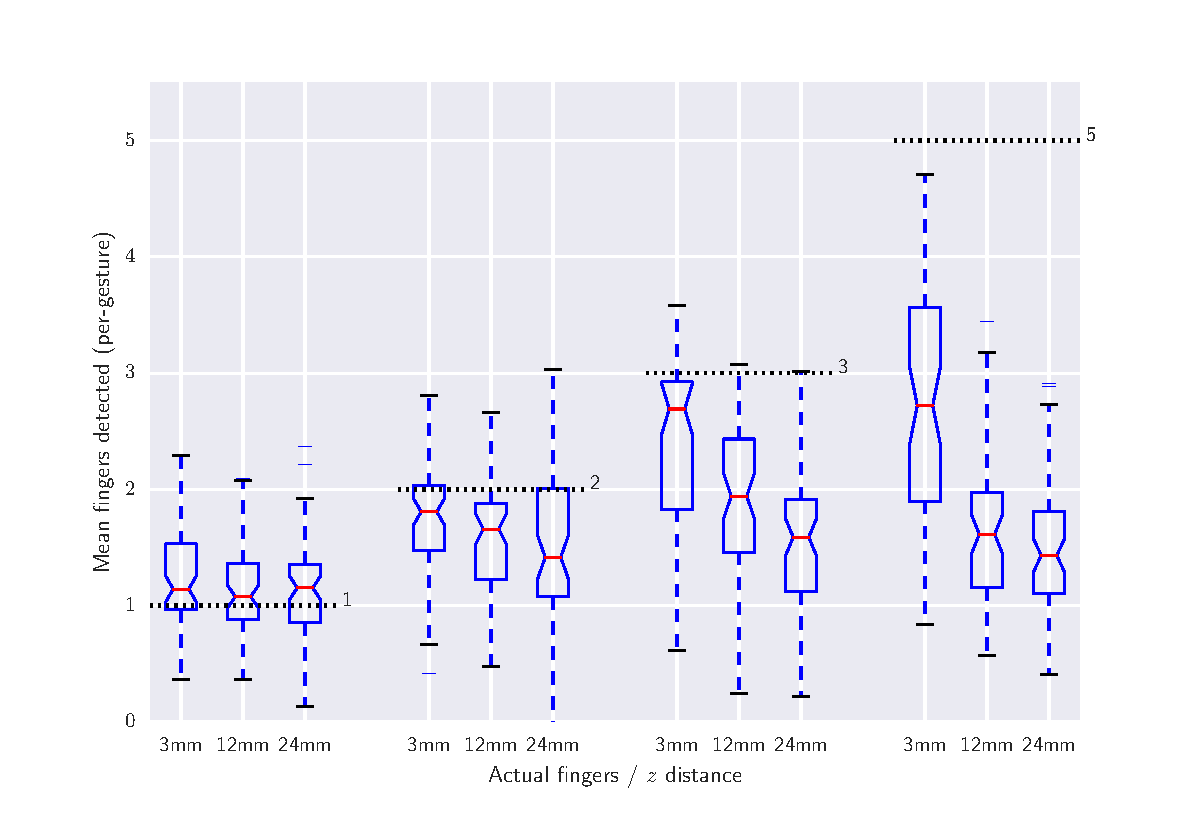
\includegraphics[width=1.0\linewidth]{images/boxplot_finger_distance.pdf}    

%     \caption{Average number of fingers detected by the touch sensor at different heights above the surface, averaged over all gestures. Dashed lines indicate
%     the true number of fingers present. The Box plots include bootstrapped uncertainty notches for the median. It is clear that the device is biased toward 
%     undercounting fingers, particularly at higher $z$ distances.
%     }

%     % use the notation fig:name to cross reference a figure
%     \label{fig:boxplot} 
% \end{figure}


% %==================================================================================================================================

\chapter{Conclusion}    
% Summarise the whole project for a lazy reader who didn't read the rest (e.g. a prize-awarding committee). This chapter should be short in most dissertations; maybe one to three pages.
% \section{Guidance}
% \begin{itemize}
%     \item
%         Summarise briefly and fairly.
%     \item
%         You should be addressing the general problem you introduced in the
%         Introduction.        
%     \item
%         Include summary of concrete results (``the new compiler ran 2x
%         faster'')
%     \item
%         Indicate what future work could be done, but remember: \textbf{you
%         won't get credit for things you haven't done}.
% \end{itemize}

\section{Summary}
% Summarise what you did; answer the general questions you asked in the introduction. What did you achieve? Briefly describe what was built and summarise the evaluation results.
In this project, we developed three builds of a video conferencing application utilising WebTransport and WebRTC. Two of these builds utilised WebTransport - out of these, one sent video data via datagrams and the other via streams. The third was a standard WebRTC build. 

We then loaded each of these builds onto a simulated network by using Mininet. Then, we altered different network quality and system metrics and evaluated how each build performed under the set conditions. We found that WebRTC outperformed both WebTransport builds, and our Streams build performed better than our Datagrams build. This achieved the project's main aim of quantitatively analysing different WebTransport (and WebRTC for comparison) builds of a video conferencing application that use different data transfer methods. 

Then, we conducted a user survey asking for participants' personal evaluations of each build. The results from this survey reflected the results from our experiments, making the survey a success in this regard. A key aim of this survey was to evaluate whether the extra development overhead of using WebTransport made a perceivable positive difference to the user or not. However, as our WebTransport builds did not outperform WebRTC, this particular question was not answered by this project as the effect on the user experience was negative. 

\section{Reflection}
% Discuss what went well and what didn't and how you would do things differently if you did this project again.
This project was certainly ambitious - we had no previous experience in developing video conferencing applications and very limited experience in developing networked applications. Because of this, development and evaluation took a lot longer than expected. We drew up a lot of ideas during the design phase that were never close to being implemented as it took us so long to meet the "must have" requirements. In particular, having builds that utilised audio and text data would have been interesting and could have led to a more comprehensive evaluation of the flexibility of WebTransport. 

In our evaluation phase, we feel that there could have been a more comprehensive and effective evaluation that simply did not happen due to time constraints. Unfortunately, it took a lot longer than expected to set up our testbed; learning the Mininet and Selenium API was harder than we had anticipated. Moreover, our decision to conduct our evaluation on a virtual machine was unwise - various bugs and reduced processing power hindered progress significantly. If we were to do this project again, we would utilise a physical machine for conducting our experiments.
In hindsight, we think there are three main weaknesses in our evaluation. Firstly, we feel that there could have been additional tests collecting more varied measurements such as frames discarded, jitter and round-trip times - these would have helped strengthen our results. This was not done simply due to lack of time. Secondly, we feel that some data being impossible to gather due to connection establishment issues in our simulated poor network conditions detracted from the scientific soundness of our evaluations. Had we more time, we would have investigated a way to establish connections in perfect network conditions and then run the experiments with the desired metrics after. Finally, conducting the experiments in a "perfect" network topology weakened our results as it made the experiments less realistic. Using a non-"perfect" network topology (i.e. sending large dummy data through switches alongside our build data) would help legitimise our results - comparing results between a perfect and non-perfect network would also make for interesting discussion. If we were to do this project again, these three weaknesses would be addressed.

Overall, we are satisfied with the project. We met our primary aim of quantitatively evaluating our builds and our results are quite strong. Developing our three builds was a valuable learning experience and although they did not all perform well, they still provided valuable insight after our evaluations and allowed us to discuss the potential of WebTransport.

\section{Future work}
% Discuss what you would do if you could take this further -- where would the interesting directions to go next be? (e.g. you got another year to work on it, or you started a company to work on this, or you pursued a PhD on this topic)
The most interesting direction to take this project would be to continue developing the WebTransport Datagrams build to address the shortcomings outlined in our experiments. We still feel that WebTransport has a lot of potential, and getting the build to a stage where it outperforms WebRTC would be interesting for many reasons. Firstly, it would be a significant development as it could help garner support for WebTransport - this is important as widespread adoption is key for the growth and potential maturation of the technology. Secondly, getting it to this stage would allow us to try to answer this project's secondary aim of evaluating whether users would even notice when a build outperforms WebRTC.

In order to achieve a more comprehensive evaluation of WebTransport's flexibility, future work should aim to include audio and text data as well as video data in our builds. Specifically, the unused "nice to have" builds outlined in our Design chapter would be interesting to implement and evaluate for the reasons stated in that chapter.

To strengthen the experiments in our evaluation, the additional tests as described in our "Reflection" section could be undertaken.

Another interesting angle that could help strengthen the case for adopting WebTransport would be to evaluate QUIC and SRTP as well as WebTransport and WebRTC. One of WebTransport's main advantages is that it uses QUIC, so including this in our evaluations would help legitimise our results and conclusions.


%==================================================================================================================================
%
% 


%==================================================================================================================================
%  APPENDICES  

\begin{appendices}

\chapter{Appendices}

\section{Wireframe}

\begin{figure}[h]
    \centering
    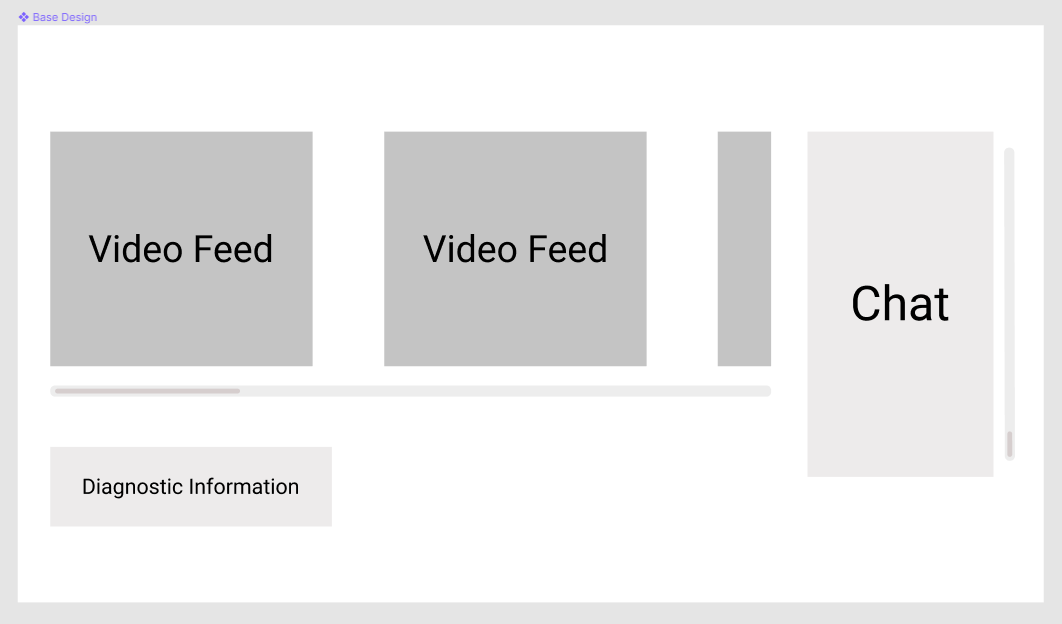
\includegraphics[width=0.7\linewidth]{images/wireframe.png}
	\caption{UI wireframe}
    \label{wireframe}
\end{figure}

\section{Build Screenshot}

\begin{figure}[h]
    \centering
    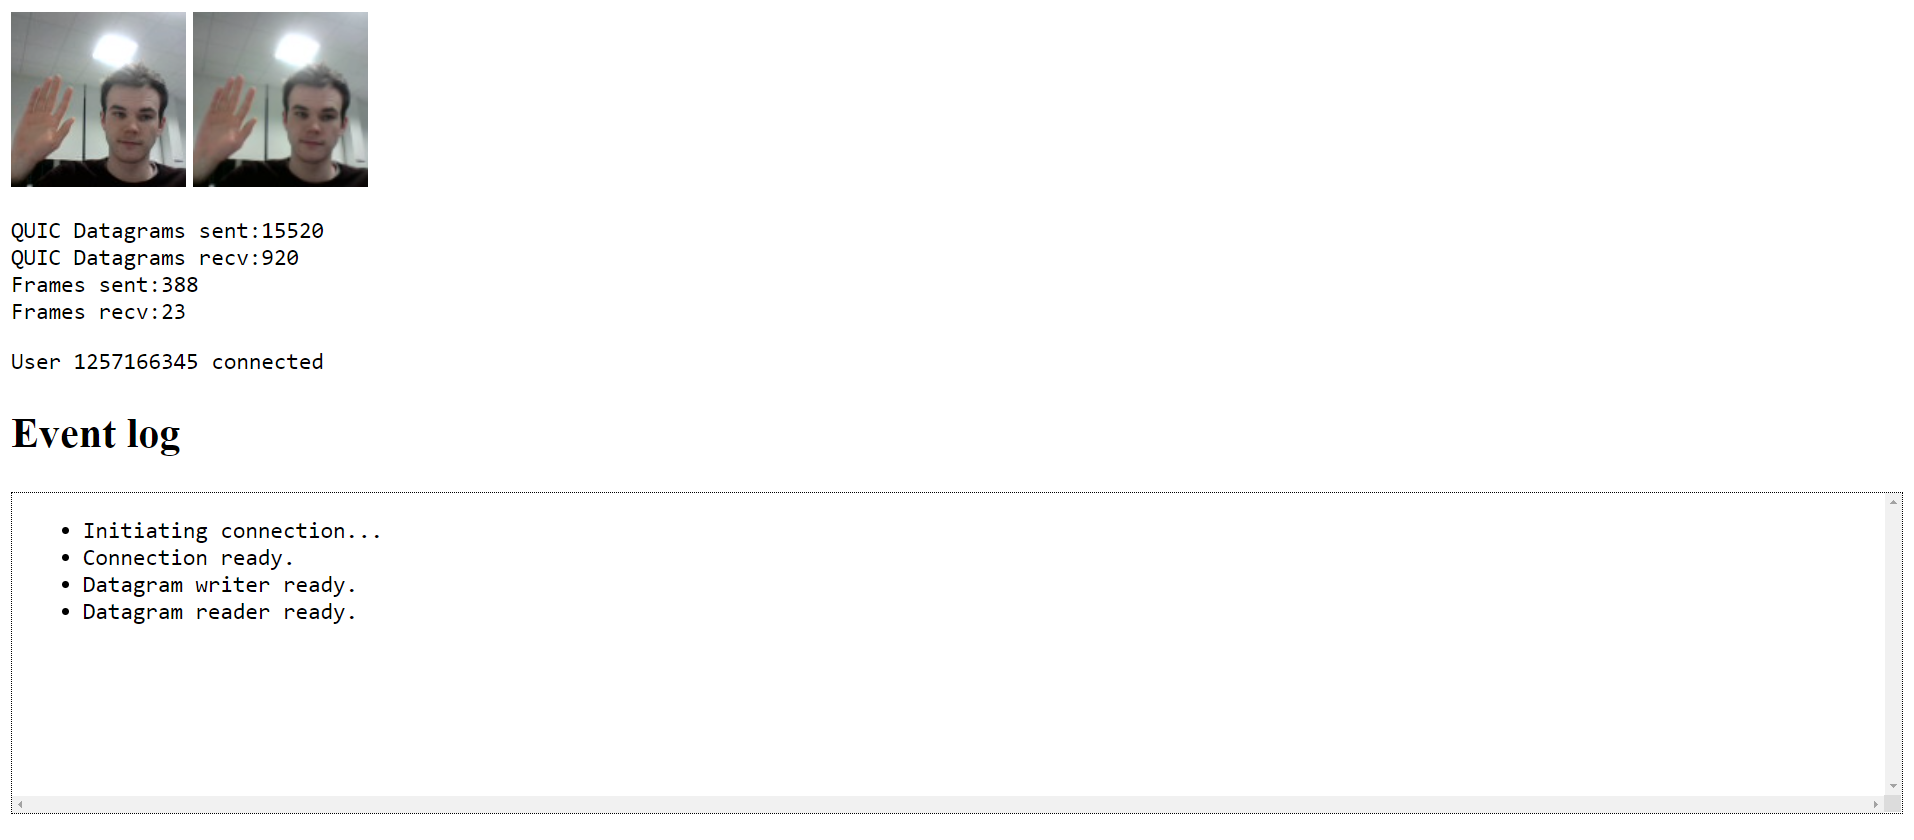
\includegraphics[width=0.95\linewidth]{images/webtransport build.png}
	\caption{A screenshot of the WebTransport Datagrams build.}
    \label{wt_build_screenshot}
\end{figure}

\section{Server Code}

\begin{lstlisting}[language=python, caption={Added server functionality that allowed the server to decode packet headers.}, label=lst:server-decode-headers]
    
class DataView:
    def __init__(self, array, bytes_per_element=1):
        self.array = array
        self.bytes_per_element = 1  # because writeBuffer is uint8 array

    def __get_binary(self, start_index, byte_count, signed=False):
        integers = [self.array[start_index + x] for x in range(byte_count)]
        bytes = [integer.to_bytes(self.bytes_per_element, byteorder='big', signed=False) for integer in integers]  
        return reduce(lambda a, b: a + b, bytes)

    def get_uint_32(self, start_index):
        bytes_to_read = 4
        return int.from_bytes(self.__get_binary(start_index, bytes_to_read), byteorder='big') 

def parse(array):
    dv = DataView(array)
    result = {
            "streamId": dv.get_uint_32(0),
            "sequenceNumber": dv.get_uint_32(4),
            "ts": dv.get_uint_32(8),
            "eof": dv.get_uint_32(12),
    }
    return result

\end{lstlisting}


\section{Experiments}
\subsection{Experiment 1 - Adjusted Bandwidth}

% Please add the following required packages to your document preamble:

\begin{table}[H]
\centering
\resizebox{\textwidth}{!}{%
\begin{tabular}{lllllll}
\cline{1-7}
Bandwidth (Mbps) & Sent Datagrams & Actual Latency (seconds) & Perceived Latency (seconds) & Received Datagrams & Loss \% & Decoding Time (seconds) \\ \cline{1-7}
100 & 1088 & 1.136301475 & 4.206732677 & 1088 & 0           & 3.070431202 \\
90  & 1061 & 1.131134778 & 3.40043     & 1061 & 0           & 2.269295222 \\
80  & 1083 & 1.001572481 & 3.433436894 & 1083 & 0           & 2.431864413 \\
70  & 1127 & 1.02790683  & 4.453066662 & 1127 & 0           & 3.425159832 \\
60  & 1100 & 0.994510907 & 3.782689326 & 1100 & 0           & 2.788178419 \\
50  & 1030 & 1.231666989 & 4.24247917  & 1030 & 0           & 3.010812181 \\
40  & 1075 & 1.073446929 & 3.428393944 & 1074 & 0.093023256 & 2.354947015 \\
30  & 1013 & 1.283492599 & 3.967178945 & 1013 & 0           & 2.683686346 \\
20  & 1027 & 0.976548199 & 3.5965625   & 1027 & 0           & 2.620014301 \\
10  & 1020 & 1.030102941 & 3.522915787 & 1020 & 0           & 2.492812846 \\
1   & 1028 & 1.734463651 & 5.145516472 & 1018 & 0.972762646 & 3.411052821 \\
0.9 & 1075 & 2.066667286 & 5.865989695 & 1070 & 0.465116279 & 3.799322409 \\
0.8 & 1073 & 2.407485418 & 6.467302079 & 1063 & 0.931966449 & 4.059816661 \\
0.7 & 1106 & 2.85741443  & 7.013072923 & 1081 & 2.26039783  & 4.155658493 \\
0.6 & 1169 & 3.723387183 & 9.637460008 & 1139 & 2.566295979 & 5.914072825 \\
0.5 & 1135 & 4.422732085 & 10.67664949 & 1116 & 1.674008811 & 6.253917405 \\
0.4 & 1290 & 6.564913738 & 13.61175228 & 1252 & 2.945736434 & 7.046838542 \\
0.3 & 1448 & 10.52214509 & 19.65060976 & 1406 & 2.900552486 & 9.12846467  \\
0.2 & 1391 & 38.4851569  & 47.80998836 & 1007 & 27.60603882 & 9.32483146  \\
0.1 & 1868 & 106.3042405 & 125.3849291 & 1455 & 22.10920771 & 19.0806886 
\end{tabular}%
}
\caption{WebTransport (Datagrams) and Adjusted Bandwidth}
\label{tab:wt-dg-bw}
\end{table}

\begin{table}[H]
\centering
\resizebox{\textwidth}{!}{%
\begin{tabular}{llll}
\cline{1-4}
Bandwidth (Mbps) & Actual Latency (seconds) & Perceived Latency (seconds) & Decoding Time (seconds)  \\ \cline{1-4}
100 & 1.649842 & 1.721053 & 0.071211 \\
90  & 0.93885  & 1.0752   & 0.13635  \\
80  & 0.77319  & 0.870286 & 0.097095 \\
70  & 0.9022   & 1.0094   & 0.1072   \\
60  & 1.7594   & 1.854    & 0.0946   \\
50  & 0.964667 & 1.040143 & 0.075476 \\
40  & 0.8306   & 0.94915  & 0.11855  \\
30  & 1.532235 & 1.661824 & 0.129588 \\
20  & 1.451182 & 1.538227 & 0.087045 \\
10  & 0.826905 & 0.937333 & 0.110429 \\
1   & 10.88552 & 11.71159 & 0.826074 \\
0.9 & 11.99833 & 12.93026 & 0.931926 \\
0.8 & 10.87782 & 11.7805  & 0.902679 \\
0.7 & 13.26152 & 14.28662 & 1.025103 \\
0.6 & 13.16544 & 14.3124  & 1.14696  \\
0.5 & 15.94833 & 17.36317 & 1.414833 \\
0.4 & 19.06361 & 20.80539 & 1.741783 \\
0.3 & 25.04241 & 27.36714 & 2.324727 \\
0.2 & 38.15827 & 41.67477 & 3.5165   \\
0.1 & 93.49667 & 103.8749 & 10.37827
\end{tabular}%
}
\caption{WebTransport Streams Build and Adjusted Bandwidth.}
\label{tab:wt-streams-bw}
\end{table}

% Please add the following required packages to your document preamble:
% \usepackage{graphicx}
\begin{table}[H]
\centering
\resizebox{\textwidth}{!}{%
\begin{tabular}{llllll}
\cline{1-6}
Bandwidth (Mbps) & Received Packets & Lost Packets & Received Frames & Dropped Frames & Decoding Time (seconds) \\ \cline{1-6}
100 & 10010 & 0 & 1236 & 0  & 0.008545307 \\
90  & 10043 & 0 & 695  & 38 & 0.078160742 \\
80  & 10071 & 0 & 610  & 0  & 0.026621311 \\
70  & 10038 & 0 & 1196 & 0  & 0.020985774 \\
60  & 10133 & 0 & 333  & 53 & 0.299902834 \\
50  & 10053 & 0 & 487  & 41 & 0.190211364 \\
40  & 10001 & 0 & 631  & 0  & 0.027101426 \\
30  & 10007 & 0 & 1112 & 0  & 0.031383993 \\
20  & 10025 & 0 & 601  & 28 & 0.162756696 \\
10  & 10025 & 0 & 1144 & 0  & 0.028993007 \\
1   & 10006 & 0 & 486  & 0  & 0.036995868 \\
0.9 & 10064 & 0 & 735  & 0  & 0.075872109 \\
0.8 & 10124 & 0 & 462  & 38 & 0.139028424 \\
0.7 & 10022 & 0 & 628  & 0  & 0.035926635 \\
0.6 & 10003 & 0 & 804  & 0  & 0.017557908 \\
0.5 & 10049 & 0 & 981  & 0  & 0.01404893  \\
0.4 & 10068 & 0 & 817  & 30 & 0.077968792 \\
0.3 & 10062 & 0 & 449  & 41 & 0.147513441 \\
0.2 & 10007 & 0 & 839  & 0  & 0.039269368 \\
0.1 & 10029 & 0 & 1107 & 0  & 0.044305606
\end{tabular}%
}
\caption{WebRTC and Adjusted Bandwidth}
\label{tab:webrtc-bw}
\end{table}

\subsection{Experiment 2 - Adjusted Latency}

\begin{table}[H]
\centering
\resizebox{\textwidth}{!}{%
\begin{tabular}{lllllll}
\cline{1-7}
Latency (ms) &
  Sent Packets &
  Actual Latency (seconds) &
  Perceived Latency (seconds) &
  Received Packets &
  Loss (percentage) &
  Decoding time (seconds) \\ \cline{1-7}
0   & 1052  & 0.976475 & 3.763616 & 1052 & 0           & 2.787141 \\
10  & 1077  & 0.874936 & 2.955848 & 1077 & 0           & 2.080913 \\
20  & 1013  & 0.876925 & 3.087404 & 1013 & 0           & 2.210479 \\
30  & 1076  & 1.016033 & 3.02558  & 1076 & 0           & 2.009547 \\
40  & 1062  & 2.668826 & 4.699883 & 1062 & 0           & 2.031057 \\
50  & 1011  & 5.331895 & 7.24175  & 1011 & 0           & 1.909855 \\
60  & 1005  & 5.803744 & 7.673044 & 1005 & 0           & 1.8693   \\
70  & 1051  & 8.46561  & 10.55796 & 1051 & 0           & 2.092348 \\
80  & 1016  & 9.080874 & 11.00218 & 1016 & 0           & 1.921311 \\
90  & 1087  & 9.916284 & 12.44948 & 1087 & 0           & 2.533201 \\
100 & 1080  & 12.11156 & 14.31101 & 1080 & 0           & 2.19945  \\
150 & 1065  & 14.59849 & 16.41119 & 486  & 54.3662     & 1.812696 \\
200 & 1052  & 12.39325 & 14.30124 & 215  & 79.56274    & 1.907984 \\
250 & 1059  & 12.14835 & 14.09013 & 130  & 87.72427    & 1.941771 \\
\end{tabular}%
}
\caption{WebTransport (Datagrams) and Adjusted Latency}
\label{tab:wt-dg-lat}
\end{table}

% Please add the following required packages to your document preamble:
% \usepackage{graphicx}
\begin{table}[H]
\centering
\resizebox{\textwidth}{!}{%
\begin{tabular}{llll}
\cline{1-4}
Latency (ms) & Perceived Latency (seconds) & Actual Latency (seconds) & Decoding time (seconds) \\ \cline{1-4}
0   & 1.025143 & 1.156857 & 0.131714 \\
10  & 1.391    & 1.542636 & 0.151636 \\
20  & 0.604238 & 0.726238 & 0.122    \\
30  & 0.622409 & 0.762545 & 0.140136 \\
40  & 4.85487  & 5.27887  & 0.424    \\
50  & 6.926783 & 7.442522 & 0.515739 \\
60  & 8.358522 & 8.970261 & 0.611739 \\
70  & 10.35474 & 11.1183  & 0.763565 \\
80  & 11.10536 & 11.90886 & 0.8035   \\
90  & 12.27232 & 13.18668 & 0.914364 \\
100 & 14.19643 & 15.182   & 0.985565 \\
150 & 14.03242 & 15.94675 & 1.914333 \\
200 & 11.62667 & 15.0285  & 3.401833 \\
250 & 10.02767 & 15.99867 & 5.971   
\end{tabular}%
}
\caption{WebTransport (Streams) and Adjusted Latency}
\label{tab:wt-streams-lat}
\end{table}

% Please add the following required packages to your document preamble:
% \usepackage{graphicx}
\begin{table}[H]
\centering
\resizebox{\textwidth}{!}{%
\begin{tabular}{llllll}
\cline{1-6}
Latency (ms) & Received Packets & Lost Packets & Received Frames & Dropped Frames & Decoding Time \\ \cline{1-6}
0   & 10078 & 0 & 563  & 43 & 0.121372414 \\
10  & 10003 & 0 & 920  & 0  & 0.029598477 \\
20  & 10006 & 0 & 1098 & 0  & 0.010996354 \\
30  & 10040 & 0 & 591  & 0  & 0.025365482 \\
40  & 10052 & 0 & 982  & 0  & 0.025781059 \\
50  & 10114 & 0 & 607  & 32 & 0.099284333 \\
60  & 10013 & 0 & 585  & 33 & 0.115221987 \\
70  & 10074 & 0 & 613  & 32 & 0.104486792 \\
80  & 10017 & 0 & 925  & 0  & 0.029551351 \\
90  & 10101 & 0 & 1107 & 0  & 0.01095208  \\
100 & 10059 & 0 & 1010 & 0  & 0.011485629 \\
150 & 10038 & 0 & 875  & 0  & 0.053164571 \\
200 & 10008 & 0 & 847  & 0  & 0.055348288 \\
250 & 10038 & 0 & 611  & 35 & 0.109828794 \\
500 & 10096 & 0 & 352  & 0  & 0.065306818
\end{tabular}%
}
\caption{WebRTC and Adjusted Latency.}
\label{tab:webrtc-lat}
\end{table}

\subsection{Experiment 3 - Adjusting Loss}

\begin{table}[H]
\centering
\resizebox{\textwidth}{!}{%
\begin{tabular}{lllllll}
\hline
Link Loss   (Percentage) & Sent Packets & Actual Latency & Perceived Latency & Received Packets & Packet Loss (Percentage) & Decoding Time (seconds) \\ \hline
0  & 1030 & 1.17875  & 5.058732 & 1030 & 0        & 3.879982 \\
1  & 1037 & 1.181895 & 4.23154  & 977  & 5.785921 & 3.049646 \\
2  & 1020 & 0.861158 & 2.968145 & 904  & 11.37255 & 2.106986 \\
3  & 1097 & 1.051883 & 3.678829 & 892  & 18.68733 & 2.626946 \\
4  & 1084 & 1.006476 & 3.042372 & 850  & 21.58672 & 2.035895 \\
5  & 1068 & 1.070334 & 3.467044 & 773  & 27.62172 & 2.39671  \\
6  & 1004 & 0.996751 & 2.853883 & 696  & 30.67729 & 1.857132 \\
7  & 1020 & 1.107166 & 4.041603 & 670  & 34.31373 & 2.934438 \\
8  & 1111 & 1.814649 & 4.7985   & 644  & 42.0342  & 2.983851 \\
9  & 1119 & 1.199182 & 3.801895 & 627  & 43.96783 & 2.602713 \\
10 & 1045 & 1.23803  & 4.057154 & 571  & 45.35885 & 2.819124 \\
11 & 1039 & 2.205973 & 5.294235 & 406  & 60.92397 & 3.088262
\end{tabular}%
}
\caption{WebTransport (Datagrams) and Adjusted Loss}
\label{tab:wt-dg-loss}
\end{table}

\begin{table}[H]
\centering
\resizebox{\textwidth}{!}{%
\begin{tabular}{llll}
\cline{1-4}
Loss (percentage) & Actual Latency (seconds) & Perceived Latency (seconds) & Decoding Time (seconds) \\ \cline{1-4}
0  & 1.032667 & 1.115    & 0.082333 \\
1  & 0.840833 & 1.153333 & 0.3125   \\
2  & 1.522783 & 1.671609 & 0.148826 \\
3  & 1.631944 & 1.799833 & 0.167889 \\
4  & 1.68384  & 1.81068  & 0.12684  \\
5  & 1.59756  & 1.74608  & 0.14852  \\
6  & 5.77372  & 6.16508  & 0.39136  \\
7  & 5.095111 & 5.528333 & 0.433222 \\
8  & 5.176346 & 5.624923 & 0.448577 \\
9  & 4.043    & 4.443647 & 0.400647 \\
10 & 3.435048 & 3.894095 & 0.459048 \\
11 & 2.259143 & 2.834    & 0.574857 \\
12 & 7.822733 & 9.092333 & 1.2696  
\end{tabular}%
}
\caption{WebTransport (Streams) and Adjusted Loss.}
\label{tab:wt-streams-loss}
\end{table}

% Please add the following required packages to your document preamble:
% \usepackage{graphicx}
\begin{table}[H]
\centering
\resizebox{\textwidth}{!}{%
\begin{tabular}{llllll}
\cline{1-6}
Loss (percentage) & Received Packets & Lost Packets & Received Frames & Dropped Frames & Decoding Time \\ \cline{1-6}
0  & 10052 & 0 & 1093 & 0  & 0.021029304 \\
1  & 10033 & 0 & 469  & 43 & 0.122772727 \\
2  & 10039 & 0 & 580  & 48 & 0.103547619 \\
3  & 10007 & 0 & 736  & 0  & 0.018910204 \\
4  & 10016 & 0 & 647  & 0  & 0.022996909 \\
5  & 10104 & 0 & 612  & 41 & 0.09699811  \\
6  & 10087 & 0 & 623  & 34 & 0.099592308 \\
7  & 10001 & 0 & 1229 & 0  & 0.007458469 \\
8  & 10189 & 0 & 601  & 35 & 0.096801066 \\
9  & 10056 & 0 & 979  & 0  & 0.029156442 \\
10 & 10085 & 0 & 608  & 30 & 0.091994526 \\
20 & 10046 & 0 & 1002 & 26 & 0.034274409
\end{tabular}%
}
\caption{WebRTC and Adjusted Loss.}
\label{tab:wrtc-loss}
\end{table}

% Use separate appendix chapters for groups of ancillary material that support your dissertation. 
% Typical inclusions in the appendices are:

% \begin{itemize}
% \item
%   Copies of ethics approvals (you must include these if you needed to get them)
% \item
%   Copies of questionnaires etc. used to gather data from subjects. Don't include
%   voluminous data logs; instead submit these electronically alongside your source code.
% \item
%   Extensive tables or figures that are too bulky to fit in the main body of
%   the report, particularly ones that are repetitive and summarised in the body.
% \item Outline of the source code (e.g. directory structure), 
%     or other architecture documentation like class diagrams.
% \item User manuals, and any guides to starting/running the software. 
% Your equivalent of \texttt{readme.md} should be included.

% \end{itemize}

% \textbf{Don't include your source code in the appendices}. It will be
% submitted separately.

\subsection{Experiment 4 - Adjusting Network Quality (Bandwidth, Latency, Loss)}

% Please add the following required packages to your document preamble:
% \usepackage{graphicx}
\begin{table}[H]
\centering
\resizebox{\textwidth}{!}{%
\begin{tabular}{llllllllll}
\cline{1-10}
Configuration Number &
  Link Loss (percentage) &
  Bandwidth (Mbps) &
  Latency (milliseconds) &
  Sent Packets &
  Actual Latency (seconds) &
  Perceived Latency (seconds) &
  Received Packets &
  Application Loss (percentage) &
  Decoding Time (seconds) \\ \cline{1-10}
1  & 0   & 100 & 0     & 1041 & 0.995932 & 3.187219 & 1041 & 0        & 2.191287 \\
2  & 0.5 & 90  & 12.5  & 1039 & 1.043007 & 3.418815 & 999  & 3.849856 & 2.375808 \\
3  & 1.5 & 80  & 25    & 1003 & 6.242995 & 9.122294 & 928  & 7.477567 & 2.879299 \\
4  & 2   & 70  & 37.5  & 1060 & 12.41988 & 14.447   & 550  & 48.11321 & 2.027118 \\
5  & 2.5 & 60  & 50    & 1028 & 10.9427  & 14.42868 & 470  & 54.28016 & 3.485983 \\
6  & 3   & 50  & 62.5  & 1061 & 13.64404 & 15.40292 & 320  & 69.83977 & 1.758886 \\
7  & 3.5 & 40  & 75    & 1183 & 22.66595 & 25.52615 & 325  & 72.52747 & 2.860203 \\
8  & 4   & 30  & 87.5  & 1344 & 26.31809 & 29.81496 & 338  & 74.85119 & 3.49687  \\
9  & 4.5 & 20  & 100   & 1073 & 18.52365 & 22.44569 & 180  & 83.2246  & 3.922042 \\
10 & 5   & 10  & 112.5 & 1281 & 42.95607 & 45.52616 & 248  & 80.64012 & 2.570089 \\
11 & 5.5 & 1   & 125   & 1153 & 29.30913 & 35.47967 & 237  & 79.44493 & 6.170536 \\
12 & 6   & 0.9 & 137.5 & 1285 & 47.06256 & 50.4007  & 239  & 81.40078 & 3.338144 \\
13 & 6.5 & 0.8 & 150   & 1092 & 50.08097 & 52.97945 & 231  & 78.84615 & 2.89848 
\end{tabular}%
}
\caption{WebTransport (Datagrams) and Adjusted Network Quality (Bandwidth, Latency and Loss)}
\label{tab:wt-dg-nwq}
\end{table}

% Please add the following required packages to your document preamble:
% \usepackage{graphicx}
\begin{table}[H]
\centering
\resizebox{\textwidth}{!}{%
\begin{tabular}{llllllllll}
\cline{1-7}
Configuration Number &
  Link Loss (percentage) &
  Bandwidth (Mbps) &
  Latency (milliseconds) &
  Actual Latency (seconds) &
  Perceived Latency (seconds) &
  Decoding Time (seconds) &
   \\ \cline{1-7}
1  & 0   & 100 & 0    & 0.6966   & 0.79348  & 0.09688  &  &  &  \\
2  & 0.5 & 90  & 12.5 & 3.47748  & 3.82252  & 0.34504  &  &  &  \\
3  & 1   & 100 & 0    & 1.442727 & 1.58     & 0.137273 &  &  &  \\
4  & 1.5 & 80  & 25   & 1.8308   & 2.8824   & 1.0516   &  &  &  \\
5  & 2   & 70  & 37.5 & 9.937667 & 11.878   & 1.940333 &  &  &  \\
6  & 2.5 & 60  & 50   & 9.179875 & 11.88813 & 2.70825  &  &  &  \\
7  & 3   & 50  & 62.5 & 10.9075  & 14.412   & 3.5045   &  &  &  \\
8  & 3.5 & 40  & 75   & 10.4802  & 15.6172  & 5.137    &  &  &  \\
9  & 4   & 30  & 87.5 & 12.8826  & 19.613   & 6.7304   &  &  &  \\
10 & 4.5 & 20  & 100  & 13.4196  & 21.3066  & 7.887    &  &  &  \\

\end{tabular}%
}
\caption{WebTransport (Streams) and Adjusted Network Quality (Bandwidth, Latency and Loss)}
\label{tab:wt-streams-nwq}
\end{table}

% Please add the following required packages to your document preamble:
% \usepackage{graphicx}
\begin{table}[H]
\centering
\resizebox{\textwidth}{!}{%
\begin{tabular}{lllllllll}
\cline{1-9}
Configuration Number &
  Loss (percentage) &
  Bandwidth (Mbps) &
  Latency (ms) &
  Received Packets &
  Packets Lost &
  Received Frames &
  Frames Dropped &
  Decoding Time (seconds) \\ \cline{1-9}
1  & 0   & 100 & 0     & 10037 & 0   & 362  & 85  & 0.219081 \\
2  & 0.5 & 90  & 12.5  & 10020 & 0   & 1014 & 0   & 0.013055 \\
3  & 1.5 & 80  & 25    & 10008 & 0   & 945  & 0   & 0.014511 \\
4  & 2   & 70  & 37.5  & 10041 & 0   & 559  & 0   & 0.116764 \\
5  & 2.5 & 60  & 50    & 10082 & 0   & 318  & 31  & 0.422052 \\
6  & 3   & 50  & 62.5  & 10025 & 27  & 314  & 18  & 0.406777 \\
7  & 3.5 & 40  & 75    & 10017 & 153 & 189  & 0   & 0.19518  \\
8  & 4   & 30  & 87.5  & 10179 & 0   & 369  & 23  & 0.18094  \\
9  & 4.5 & 20  & 100   & 10037 & 0   & 633  & 0   & 0.020564 \\
10 & 5   & 10  & 112.5 & 10009 & 0   & 389  & 115 & 0.195751 \\
11 & 5.5 & 1   & 125   & 10116 & 0   & 328  & 24  & 0.238981 \\
12 & 6   & 0.9 & 137.5 & 10033 & 0   & 500  & 0   & 0.074302 \\
13 & 6.5 & 0.8 & 150   & 10160 & 0   & 359  & 31  & 0.200252 \\
14 & 7   & 0.7 & 162.5 & 10037 & 0   & 544  & 0   & 0.065722 \\
15 & 7.5 & 0.6 & 175   & 10023 & 0   & 509  & 0   & 0.037207 \\
16 & 8   & 0.5 & 187.5 & 10076 & 0   & 289  & 39  & 0.241652 \\
17 & 8.5 & 0.4 & 200   & 10009 & 4   & 663  & 2   & 0.023171 \\
18 & 9   & 0.3 & 212.5 & 10025 & 21  & 490  & 66  & 0.155466 \\
19 & 9.5 & 0.2 & 225   & 10060 & 0   & 658  & 0   & 0.029611 \\
20 & 10  & 0.1 & 237.5 & 10005 & 0   & 558  & 0   & 0.065294
\end{tabular}%
}
\caption{WebRTC and Adjusted Network Quality (Bandwidth, Latency and Loss)}
\label{tab:wrtc-nwq}
\end{table}

\subsection{Experiment 5 - Adjusting CPU Usage}
% Please add the following required packages to your document preamble:
% \usepackage{graphicx}

\begin{table}[H]
\centering
\resizebox{\textwidth}{!}{%
\begin{tabular}{lllllll}
\cline{1-7}
CPU Usage (percentage) &
  Sent Packets &
  Actual Latency (seconds) &
  Perceived Latency (seconds) &
  Received Packets &
  Loss (percentage) &
  Decoding Time (seconds) \\ \cline{1-7}
100 & 1005 & 0.843825 & 3.191516 & 1005 & 0        & 2.347691 \\
90  & 1091 & 5.716807 & 17.91599 & 1081 & 0.91659  & 12.19918 \\
80  & 1123 & 6.129455 & 16.55441 & 1123 & 0        & 10.42496 \\
70  & 1158 & 7.535191 & 17.6615  & 1158 & 0        & 10.12631 \\
60  & 1406 & 10.63798 & 25.1972  & 1395 & 0.782361 & 14.55922 \\
50  & 1054 & 7.103321 & 19.56197 & 1009 & 4.26945  & 12.45864 \\
40  & 1051 & 1.031816 & 3.963888 & 1051 & 0        & 2.932071 \\
30  & 1008 & 1.530039 & 6.713181 & 1008 & 0        & 5.183142 \\
20  & 1051 & 6.363102 & 17.89056 & 1051 & 0        & 11.52746 \\
10  & 324  & 37.08473 & 54.46188 & 307  & 5.246914 & 17.37716 \\
    &      &          &          &      &          &          \\
    &      &          &          &      &          &         
\end{tabular}%
}
\caption{WebTransport (Datagrams) and Adjusted CPU Usage}
\label{tab:wt-dg-cpu}
\end{table}

% Please add the following required packages to your document preamble:
% \usepackage{graphicx}
\begin{table}[H]
\centering
\resizebox{\textwidth}{!}{%
\begin{tabular}{lllllll}
\cline{1-4}
CPU Usage (percentage) & Actual Latency (seconds) & Perceived Latency (seconds) & Decoding Time (seconds) &  &  &  \\ \cline{1-4}
100 & 0.46128  & 0.49028  & 0.029    &  &  &  \\
90  & 0.5764   & 0.62072  & 0.04432  &  &  &  \\
80  & 0.430417 & 0.492625 & 0.062208 &  &  &  \\
70  & 0.43328  & 0.4506   & 0.01732  &  &  &  \\
60  & 0.39476  & 0.4252   & 0.03044  &  &  &  \\
50  & 0.49832  & 0.5346   & 0.03628  &  &  &  \\
40  & 1.951348 & 2.192    & 0.240652 &  &  &  \\
30  & 1.005909 & 1.134682 & 0.128773 &  &  &  \\
20  & 1.863    & 2.076957 & 0.213957 &  &  &  \\
10  & 5.56887  & 6.098652 & 0.529783 &  &  &  \\
    &          &          &          &  &  &  \\
    &          &          &          &  &  & 
\end{tabular}%
}
\caption{WebTransport (Streams) and Adjusted CPU Usage}
\label{tab:wt-streams-cpu}
\end{table}

% Please add the following required packages to your document preamble:
% \usepackage{graphicx}
\begin{table}[H]
\centering
\resizebox{\textwidth}{!}{%
\begin{tabular}{lllllll}
\cline{1-6}
CPU Usage (percentage) & Received Packets & Lost Packets & Received Frames & Dropped Frames & Decoding Time (seconds) &  \\ \cline{1-6}
100 & 10041 & 0 & 633  & 40  & 0.054896 &  \\
90  & 10048 & 0 & 1431 & 0   & 0.006377 &  \\
80  & 10052 & 0 & 1291 & 0   & 0.008763 &  \\
70  & 10023 & 0 & 1067 & 0   & 0.00482  &  \\
60  & 10040 & 0 & 814  & 90  & 0.117165 &  \\
50  & 10007 & 0 & 728  & 82  & 0.138772 &  \\
40  & 10031 & 0 & 1095 & 0   & 0.018466 &  \\
30  & 10052 & 0 & 637  & 101 & 0.106019 &  \\
    &       &   &      &     &          &  \\
    &       &   &      &     &          &  \\
    &       &   &      &     &          &  \\
    &       &   &      &     &          & 
\end{tabular}%
}
\caption{WebRTC and Adjusted CPU Usage}
\label{tab:wrtc-cpu}
\end{table}

\section{User Survey Ethics Form}

\begin{figure}[h]
    \centering
    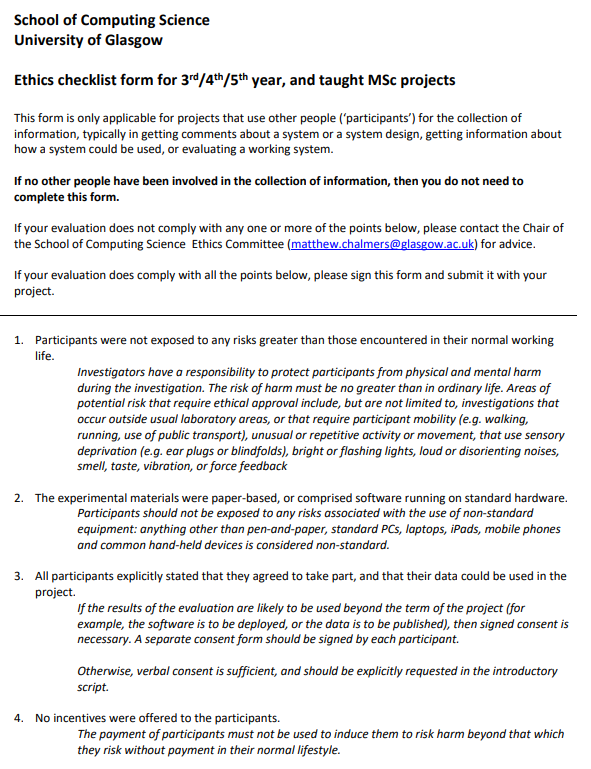
\includegraphics[width=0.95\linewidth]{images/ethics/checklist-1.png}
	\caption{Signed ethics checklist - Part 1.}
    \label{ethics-1}
\end{figure}

\begin{figure}[h]
    \centering
    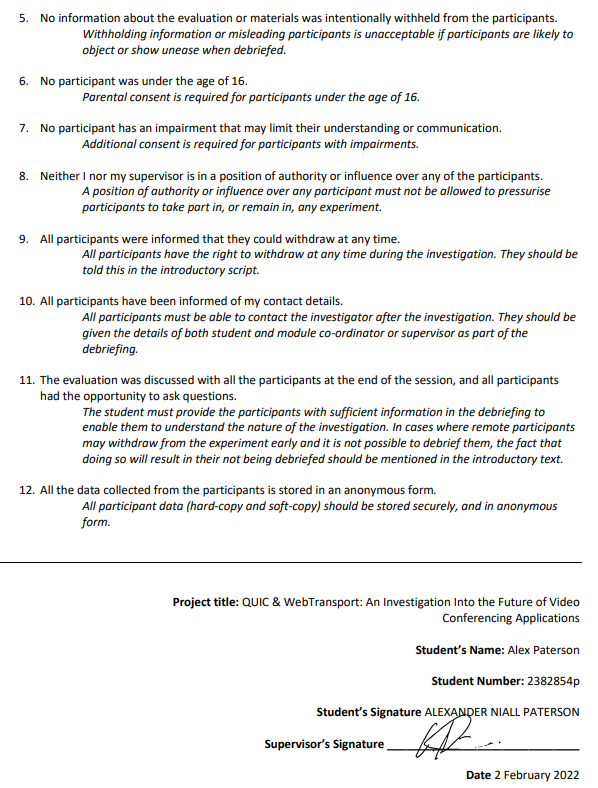
\includegraphics[width=0.95\linewidth]{images/ethics/checklist-2.png}
	\caption{Signed ethics checklist - Part 2.}
    \label{ethics-2}
\end{figure}


\end{appendices}

%==================================================================================================================================
%   BIBLIOGRAPHY   

% The bibliography style is agsm (Harvard)
% The bibliography always appears last, after the appendices.


% \bibliographystyle{agsm}

% % Force the bibliography not to be numbered
% \renewcommand{\thechapter}{0} 
% \bibliography{l4proj.bib}
\printbibliography


\end{document}
